\documentclass[12pt]{book}
\usepackage{html,a4wide,epsfig}
\usepackage[british]{babel}
\newcommand{\hl}[1]{\htmladdnormallink{{\it #1}}{#1}}
\newcommand{\ix}[1]{#1\index{#1}}
\newcommand{\linecmd}{
   \setlength{\unitlength}{1cm}
   \noindent
   \begin{picture}(18,0.12)
     \thicklines
     \put(0,0){\line(1,0){17}}
     \put(0,0.1){\line(1,0){17}}
   \end{picture}
}
\newcommand{\idxcmd}[1]{
   \addcontentsline{toc}{subsubsection}{#1}
   \index{#1}
}

\makeindex
\begin{document}
\pagenumbering{roman}
\pagestyle{empty}
\addtocontents{toc}{\protect\setcounter{tocdepth}{3}}

\begin{center}
{\Huge\bf SWAN}
\end{center}
\vspace{2cm}
\begin{center}
{\Large\bf USER MANUAL}
\end{center}
\vfill
\begin{center}
{\Large\bf SWAN Cycle III version 40.81}
\end{center}

\cleardoublepage

\noindent
{\Large\bf SWAN USER MANUAL}

\vfill

\begin{table}[htb]
\begin{tabular}{lcl}
by           &:& The SWAN team \\
             & & \\
mail address &:& Delft University of Technology \\
             & & Faculty of Civil Engineering and Geosciences \\
             & & Environmental Fluid Mechanics Section \\
             & & P.O. Box 5048 \\
             & & 2600 GA Delft \\
             & & The Netherlands \\
             & & \\
e-mail       &:& swan-info-citg@tudelft.nl \\
home page    &:& \hl{http://www.swan.tudelft.nl}
\end{tabular}
\end{table}

\vfill

\noindent
Copyright (c) 1993-2010 Delft University of Technology.
\\[2ex]
\noindent
Permission is granted to copy, distribute and/or modify this document
under the terms of the GNU Free Documentation License, Version 1.2
or any later version published by the Free Software Foundation;
with no Invariant Sections, no Front-Cover Texts, and no Back-Cover
Texts. A copy of the license is available at
\hl{http://www.gnu.org/licenses/fdl.html\#TOC1}.

\clearpage
\pagestyle{myheadings}
\newcommand{\chap}[1] % Re-define the chapter command for chapters
       {
        \chapter{#1}
        \markboth{\hfill Chapter \thechapter \hfill}{\hfill {#1} \hfill}
       }
\newcommand{\achap}[1] % Re-define the chapter command for appendices
       {
        \chapter{#1}
        \markboth{\hfill Appendix \thechapter \hfill}{\hfill {#1} \hfill}
       }

\tableofcontents

\chap{Introduction} \label{ch:intro}
\pagenumbering{arabic}

The information about the SWAN package is distributed over four different documents. This User Manual describes
the complete input and usage of the SWAN package. The Implementation Manual explains the installation procedure
of SWAN on a single- or multi-processor machine with shared or distributed memory. The Programming rules is meant
for programmers who want to develop SWAN. The Scientific/Technical documentation discusses the physical and
mathematical details and the discretizations that are used in the SWAN program. The mapping of these numerical
techniques in SWAN code is also discussed.
\nocite{Impman,Progrul,Techdoc}
\\[2ex]
\noindent
In Chapter~\ref{ch:defin} some general definitions and remarks concerning the usage of SWAN, the treatment of grids,
boundary conditions, etc. is given. It is advised to read these definitions and remarks before consulting the rest
of the manual. Chapter~\ref{ch:inout} gives some remarks concerning the input and output files of SWAN.
Chapter~\ref{ch:comm} describes the complete set of commands of the program SWAN.
\\[2ex]
\noindent
It is strongly advised that users who are not so experienced in the use of SWAN first read Chapters~\ref{ch:defin}
and \ref{ch:inout}.
\\[2ex]
\noindent
This Manual also contains some appendices. In Appendix~\ref{app:defvar} definitions of several output parameters are given.
Appendix~\ref{app:syntax} outlines the syntax of the command file (or input file). A complete set of all the commands use
in SWAN can be found in Appendix~\ref{app:swanedt}. Appendix~\ref{app:spcform} described the format of the files for
spectral input and output by SWAN.

\chap{General definitions and remarks} \label{ch:defin}

\section{Introduction}
The purpose of this chapter is to give some general advice in choosing the basic input for SWAN
computations.
\\[2ex]
\noindent
SWAN is a third-generation wave model for obtaining realistic estimates of wave parameters in coastal areas, lakes and
estuaries from given wind, bottom and current conditions. However, SWAN can be used on any scale relevant for
wind-generated surface gravity waves. The model is based on the wave action balance equation with sources and sinks.
\\[2ex]
\noindent
An important question addressed is how to choose various grids in SWAN (resolution, orientation,
etc.) including nesting.
In general, we consider two types of grids: structured and unstructured. Structured grids may be recti-linear and
uniform or curvi-linear. They always consist of quadrilaterals in which the number of grid cells that meet each
other in an internal grid point is 4. In unstructured grids, this number can be arbitrarily (usually between 4 and 10).
For this reason, the level of flexibility with respect to the grid point distribution of unstructured grids
is far more optimal compared to structured grids.
Unstructured grids may contain triangles or a combination of triangles and quadrilaterals (so-called hybrid grids).
In the current version of SWAN, however, only triangular meshes can be employed.
\\[2ex]
\noindent
Often, the characteristic spatial scales of the wind waves propagating from deep to shallow waters are very
diverse and would required to allow local refinement of the mesh near the coast without incurring
overhead associated with grid adaptation at some distance offshore. Traditionally, this can be achieved by employing
a nesting approach.
\\[2ex]
\noindent
The idea of nesting is to first
compute the waves on a coarse grid for a larger region and then on a finer grid for a smaller
region. The computation on the fine grid uses boundary conditions that are generated by the
computation on the coarse grid. Nesting can be repeated on ever decreasing scales using the
same type of coordinates for the coarse computations and the nested computations (Cartesian or
spherical). Note that curvi-linear grids can be used for nested computations but the boundaries
should always be rectangular.
\\[2ex]
\noindent
The use of unstructured grids in SWAN offers a good alternative to nested models not only because of the
ease of optimal adaption of mesh resolution but also the modest effort needed to generate
grids about complicated geometries, e.g. islands and irregular shorelines. This type of flexible
meshes is particularly useful in coastal regions where the water depth varies greatly. As a result,
this variable spatial meshing gives the highest resolution where it is most needed. The use of unstructured
grids facilitates to resolve the model area with a relative high accuracy but with a much fewer grid
points than with regular grids.
\\[2ex]
\noindent
It must be pointed out that the application of SWAN on ocean scales is not recommended from an
efficiency point of view. The WAM model and the WAVEWATCH~III model, which have been designed
specifically for ocean applications, are probably one order of magnitude more efficient than
SWAN. SWAN can be run on large scales (much larger than coastal scales) but this option is
mainly intended for the \underline{transition} from ocean scales to coastal scales (transitions
where nonstationarity is an issue and spherical coordinates are convenient for nesting).
\\[2ex]
\noindent
A general suggestion is: \underline{start simple}. SWAN helps in this with default options.
Furthermore, suggestions are given that should help the user to choose among the many options
conditions and in which mode to run SWAN (first-, second- or third-generation mode, stationary
or nonstationary and 1D or 2D).

\section{Limitations}

The DIA approximation for the {\bf quadruplet wave-wave interactions} depends on the width of the directional
distribution of the wave spectrum. It seems to work reasonably in many cases but it is a poor
approximation for long-crested waves (narrow directional distribution). It also depends on the frequency
resolution. It seems to work reasonably in many cases but it is a poor approximation for frequency
resolutions with ratios very different from 10\% (see command {\tt CGRID}). This is a fundamental problem
that SWAN shares with other third-generation wave models such as WAM and WAVEWATCH~III.
\\[2ex]
\noindent
The LTA approximation for the {\bf triad wave-wave interactions} depends on the width of the directional
distribution of the wave spectrum. The present tuning in SWAN (the default settings, see command
{\tt TRIAD}) seems to work reasonably in many cases but it has been obtained from observations in a narrow
wave flume (long-crested waves).
\\[2ex]
\noindent
As an option SWAN computes {\bf wave-induced set-up}. In 1D cases the computations are
based on exact equations. In 2D cases, the computations are based on approximate equations.
This approximation in SWAN can \underline{only} be applied to open coast (unlimited supply of water from outside
the domain, e.g. nearshore coasts and estuaries) in contrast to closed basin, e.g. lakes, where this option
should not be used.
The effects of wave-induced currents are always ignored.
\\[2ex]
\noindent
SWAN does not calculate {\bf wave-induced currents}. If relevant, such currents should be provided as input
to SWAN, e.g. from a circulation model which can be driven by waves from SWAN in an iteration procedure.
\\[2ex]
\noindent
In areas where variations in wave height are large within a horizontal scale of a few wave lengths,
{\bf diffraction} should be used. However, the computation of diffraction
in arbitrary geophysical conditions is rather complicated and requires considerable computing effort. To
avoid this, a phase-decoupled approach is employed in SWAN so that same qualitative behaviour of spatial redistribution
and changes in wave direction is obtained.
This approach, however, does not properly handle diffraction in harbours
or in front of reflecting obstacles.
\\[2ex]
\noindent
SWAN can be used on {\bf any scale} relevant for wind generated surface gravity waves. However, SWAN is
specifically designed for coastal applications that should actually not require such flexibility in scale. The
reasons for providing SWAN with such flexibility are:
\begin{itemize}
  \item to allow SWAN to be used from laboratory conditions to shelf seas and
  \item to nest SWAN in the WAM model or the WAVEWATCH~III model which are formulated in terms of
        spherical coordinates.
\end{itemize}
Nevertheless, these facilities are not meant to support the use of SWAN on oceanic scales because
SWAN is less efficient on oceanic scales than WAVEWATCH~III and probably also less efficient than WAM.

\section{Internal scenarios, limiters, shortcomings and coding bugs}

Sometimes the user input to SWAN is such that SWAN produces unreliable and sometimes even
unrealistic results. This may be the case if the bathymetry or the wave field is not well resolved. Be aware
here that the grid on which the computations are performed interpolates from the grids on which the input
is provided; different resolutions for these grids (which are allowed) can therefore create unexpected
interpolation patterns on the computational grid. In such cases SWAN may invoke some {\bf internal
scenarios} or {\bf limiters} instead of terminating the computations. The reasons for this model policy is that
\begin{itemize}
  \item SWAN needs to be robust, and
  \item the problem may be only very local, or
  \item the problem needs to be fully computed before it can be diagnosed.
\end{itemize}

Examples are:
\begin{itemize}
  \item The user can request that \underline{refraction} over one spatial grid step is limited to about
        90$^{{\rm 0}}$(see command {\tt NUMERIC}). This may be relevant when the depth varies considerably
        over one spatial grid step (e.g. at the edge of oceans or near oceanic islands with only
        one or two grid steps to go from oceanic depths to a shallow coast). This implies
        inaccurate refraction computations in such grid steps. This may be acceptable when
        refraction has only local effects that can be ignored but, depending on the topography,
        the inaccurately computed effects may radiate far into the computational area.
  \item SWAN cannot handle wave propagation on \underline{super-critical current flow}. If such flow is
        encountered during SWAN computations, the current is locally reduced to sub-critical flow.
  \item If the \underline{water depth} is less than some user-provided limit, the depth is set at that limit
        (default is 0.05 m, see command {\tt SET}).
  \item The \underline{user-imposed wave boundary conditions} may not be reproduced by SWAN,
        as SWAN replaces the {\it imposed} waves at the boundaries that
        propagate into the computational area with the {\it computed} waves that move out of the computational
        area at the boundaries.
  \item SWAN may have \underline{convergence} problems. There are three iteration processes in SWAN:
        \begin{enumerate}
           \item an iteration process for the spatial propagation of the waves,
           \item if ambient currents are present, an iteration process for spectral propagation
                 (current-induced refraction and frequency shift) and
           \item if wave-induced set-up is requested by the user, an iteration process for
                 solving the set-up equation.
        \end{enumerate}
        \begin{itemize}
           \item[ad 1] For spatial propagation the change of the wave field over one iteration is
                       limited to some realistic value (usually several iterations for stationary
                       conditions or one iteration or upgrade per time step for nonstationary
                       conditions; see command {\tt NUMERIC}). This is a common problem for all
                       third-generation wave models (such as WAM, WAVEWATCH~III and also SWAN). It
                       does not seem to affect the result seriously in many cases but sometimes
                       SWAN fails to converge properly.
                       \\[2ex]
                       \noindent
                       For curvi-linear grids, convergence problems may occur locally where in some
                       points in the grid, the directions separating the 4 sweeping quadrants coincide
                       with the given spectral directions.
           \item[ad 2] For spectral propagation (but only current-induced refraction and frequency
                       shift) SWAN may also not converge.
           \item[ad 3] For the wave-induced set-up SWAN may also not converge.
         \end{itemize}
         Information on the actual convergence of a particular SWAN run is provided in the
         {\tt PRINT} file (see SWAN Implementation Manual).
\end{itemize}
Some other problems which the SWAN user may encounter are due to more {\bf fundamental shortcomings}
of SWAN (which may or may not be typical for third-generation wave models) and unintentional {\bf coding
bugs}.
\\[2ex]
\noindent
Because of the issues described above, the results may look realistic, but they may (locally) not be
accurate. Any change in these scenarios, limiters or shortcomings, in particular newly discovered coding
bugs and their fixes, are published on the SWAN web site and implemented in new releases of SWAN.

\section{Relation to WAM, WAVEWATCH~III and others}
The basic scientific philosophy of SWAN is identical to that of WAM (Cycle 3 and 4). SWAN is a third-generation
wave model and it uses the same formulations for the source terms (although SWAN uses the adapted code for the
DIA technique). On the other hand, SWAN contains some additional formulations primarily for shallow water.
Moreover, the numerical techniques are very different. WAVEWATCH~III not only uses different numerical techniques
but also different formulations for the wind input and the whitecapping.
\\[2ex]
\noindent
This close similarity can be exploited in the sense that
\begin{itemize}
  \item scientific findings with one model can be shared with the others and
  \item SWAN can be readily nested in WAM and WAVEWATCH~III (the formulations of WAVEWATCH~III
        have not yet been implemented in SWAN).
\end{itemize}
When SWAN is nested in WAM or WAVEWATCH~III, it must be noted that the boundary conditions for
SWAN provided by WAM or WAVEWATCH~III may not be model consistent even if the same physics are
used. The potential reasons are manifold such as differences in numerical techniques employed and
implementation for the geographic area (spatial and spectral resolutions, coefficients, etc.). Generally,
the deep water boundary of the SWAN nest must be located in WAM or WAVEWATCH~III  where shallow
water effects do not dominate (to avoid too large discontinuities between the two models). Also, the
spatial and spectral resolutions should not differ more than a factor two or three. If a finer resolution is
required, a second or third nesting may be needed.

\section{Units and coordinate systems}
\label{sec:units}

SWAN expects all quantities that are given by the user to be expressed in S.I. units:
m, kg, s and composites of these with accepted compounds, such as Newton
(N) and Watt (W). Consequently, the wave height and water depth are in m,
wave period in s, etc. For \underline{wind and wave direction} both the
Cartesian and {\em a} nautical convention can be used (see below). Directions and spherical
coordinates are in degrees ($^{{\rm 0}}$) and not in radians.
\\[2ex]
\noindent
For the output of wave energy the user can choose between variance (m$^{{\rm 2}}$) or energy
({\bf spatial}) density (Joule/m$^{{\rm 2}}$, i.e. energy per unit sea surface) and the
equivalents in case of energy transport (m$^{{\rm 3}}$/s or W/m, i.e. energy transport per unit
length) and spectral energy density (m$^{{\rm 2}}$/Hz/Degr or Js/m$^{{\rm 2}}$/rad, i.e. energy
per unit frequency and direction per unit sea surface area). The wave$-$induced stress
components (obtained as spatial derivatives of wave-induced radiation stress) are always expressed
in N/m$^2$ even if the wave energy is in terms of variance. Note that the energy density is also in
Joule/m$^{{\rm 2}}$ in the case of spherical coordinates.
\\[2ex]
\noindent
SWAN operates either in a Cartesian coordinate system or in a spherical coordinate system, i.e.
in a flat plane or on a spherical Earth. In the Cartesian system, all geographic locations and
orientations in SWAN, e.g. for the bottom grid or for output points, are defined in one common
Cartesian coordinate system with origin (0,0) by definition. This \underline{geographic origin
may be chosen totally arbitrarily by the user}. In the spherical system, all geographic locations
and orientations in SWAN, e.g. for the bottom grid or for output points, are defined in geographic
longitude and latitude. Both coordinate systems are designated in this manual as the
\underline{problem coordinate system}.
\\[2ex]
\noindent
In the input and output of SWAN the \underline{direction of wind and waves} are defined according to either
\begin{itemize}
 \item the \underline{Cartesian convention}, i.e. the direction to where the vector points, measured
       counterclockwise from the positive $x-$axis of this system (in degrees) or
 \item a \underline{nautical convention} (there are more such conventions), i.e. the direction where
       the wind or the waves come \underline{from}, measured clockwise from geographic North.
\end{itemize}
All \underline{other directions}, such as orientation of grids, are according to the Cartesian convention!
\\[2ex]
\noindent
For regular grids, i.e. uniform and rectangular, Figure~\ref{fig:compdom} (in Section~\ref{sec:moddesc})
shows how the locations of the various grids are determined with respect to the problem coordinates.
All grid points of curvi-linear and unstructured grids are relative to the problem coordinate system.

\section{Choice of grids, time windows and boundary / initial / first guess conditions}
\label{sec:choigrd}

\subsection{Introduction}

Several types of grids and time window(s) need to be defined: (a) spectral grid, (b) spatial (geographic)
grids and time window(s) in case of nonstationary computations.
\\[2ex]
\noindent
The {\bf spectral} grid that need to be defined by the user is a \underline{computational} spectral grid on
which SWAN performs the computations.
\\[2ex]
\noindent
SWAN has the option to make computations that can be nested in (coarse) SWAN, WAM or WAVEWATCH
III. In such cases, the spectral grid need not be equal to the spectral grid in the coarse SWAN, WAM or
WAVEWATCH~III run.
\\[2ex]
\noindent
The {\bf spatial} grids that need to be defined by the user are (if required):
\begin{itemize}
 \item a \underline{computational} spatial grid on which SWAN performs the computations,
 \item one (or more) spatial \underline{input} grid(s) for the bottom, current field, water level,
       bottom friction and wind (each input grid may differ from the others) and
 \item one (or more) spatial \underline{output} grid(s) on which the user requires output of SWAN.
\end{itemize}
The wind and bottom friction do not require a grid if they are uniform over the area of interest.
\\[2ex]
\noindent
For one-dimensional situations, i.e. $\partial /\partial y \equiv 0$, SWAN can be run in 1D mode.
\\[2ex]
\noindent
If a uniform, rectangular computational spatial grid is chosen in SWAN, then all input and output
grids must be uniform and rectangular too, but they may all be different from each other.
\\[2ex]
\noindent
If a curvi-linear computational spatial grid is chosen in SWAN, then \underline{each} input grid
should be either uniform, rectangular or identical to the used curvi-linear grid or staggered with
respect to the curvi-linear computational grid.
\\[2ex]
\noindent
If an unstructured computational spatial grid is chosen in SWAN, then \underline{each} input grid
should be either uniform, rectangular or identical to the used unstructured grid.
\\[2ex]
\noindent
SWAN has the option to make computations that are nested in (coarse) SWAN, WAM or WAVEWATCH~III.
In such runs, SWAN interpolates the spatial boundary of the SWAN, WAM or WAVEWATCH~III grid to the
(user provided) grid of SWAN (that needs to (nearly) coincide along the grid lines of WAM or WAVEWATCH
III or the output nest grid boundaries of SWAN). Since, the computational grids of WAM and WAVEWATCH
III are in spherical coordinates, it is recommended to use spherical coordinates in a nested SWAN when
nesting in WAM or WAVEWATCH~III.
\\[2ex]
\noindent
SWAN using an \underline{unstructured mesh} may be nested in SWAN employing a \underline{regular grid} and
vice versa. However, SWAN using an unstructured grid cannot be nested in WAM or WAVEWATCH~III.
\\[2ex]
\noindent
Nesting from a 2D model to a 1D model is possible although is should not be done by using the
commands {\tt NGRID} and {\tt NEST}. Instead, define the boundary point of the 1D model as an output
point (using command {\tt POINTS}) and write the spectra for that point using the command {\tt SPECout}.
In the 1D model, this spectra is used as boundary condition using the {\tt BOUNDSPEC} command.
\\[2ex]
\noindent
Similarly, the wind fields may be available in different {\bf time} windows than the current and water
level fields and the computations may need to be carried out at other times than these input fields.
For these reasons SWAN operates with different time windows with different time steps (each may have
a different start and end time and time step):
\begin{itemize}
  \item one \underline{computational time window} in which SWAN performs the computations,
  \item one (or more) \underline{input time window(s)} in which the bottom, current field, water level,
        bottom friction and wind field (if present) are given by the user (each input window may differ
        form the others) and
  \item one (or more) \underline{output time window(s)} in which the user requires output of SWAN.
\end{itemize}
In case of nesting, SWAN searches the boundary conditions in the relevant output file of the previous
SWAN, WAM or WAVEWATCH~III runs to take the boundary conditions at the start time of the nested run.
It will not take the initial condition (i.e. over the entire computational grid) for the nested run
from the previous SWAN, WAM or WAVEWATCH~III run.
\\[2ex]
\noindent
During the computation SWAN obtains bottom, current, water level, wind and bottom friction information
by tri-linear {\bf interpolation} from the given input grid(s) and time window(s). The output is in turn
obtained in SWAN by bi-linear interpolation in space from the computational grid; there is no interpolation
in time, the output time is shifted to the nearest computational time level. Interpolation errors can be
reduced by taking the grids and windows as much as equal to one another as possible (preferably identical).
It is recommended to choose output times such that they coincide with computational time levels.

\subsection{Input grid(s) and time window(s)}
The bathymetry, current, water level, bottom friction and wind (if spatially variable) need to be provided to
SWAN on so-called input grids. It is best to make an input grid so large that it completely covers the
computational grid.
\\[2ex]
\noindent
In the region outside the input grid SWAN assumes that the bottom level, the water level and bottom
friction are identical to those at the nearest boundary of the input grid (lateral shift of that boundary).
In the regions not covered by this lateral shift (i.e. in the outside quadrants of the corners of the input
grid), a constant field equal to the value at the nearest corner point of the input grid is taken. For the
current and wind velocity, SWAN takes 0 m/s for points outside the input grid.
\\[2ex]
\noindent
In SWAN, the bathymetry, current, water level, wind and bottom friction may be time varying. In that case
they need to be provided to SWAN in so-called input time windows (they need not be identical with the
computational, output or other input windows). It is best to make an input window larger than the
computational time window. SWAN assumes zero values at times before the earliest begin time of the
input parameters (which may be the begin time of any input parameter such as wind). SWAN assumes
constant values (the last values) at times after the end time of each input parameter. The input windows
should start early enough so that the initial state of SWAN has propagated through the computational area
before reliable output of SWAN is expected.
\\[2ex]
\noindent
One should choose the spatial resolution for the input grids such that relevant spatial details in the
bathymetry, currents, bottom friction and wind are properly resolved. Special care is required in cases with
sharp and shallow ridges (sand bars, shoals) in the sea bottom and extremely steep bottom slopes. Very
inaccurate bathymetry can result in very inaccurate refraction computations the results of which can
propagate into areas where refraction as such is not significant (the results may appear to be unstable).
For instance, waves skirting an island that is poorly resolved may propagate beyond the island with
entirely wrong directions. In such a case it may even be better to deactivate the refraction computations
(if refraction is irrelevant for the problem at hand e.g. because the refracted waves will run into the coast
anyway and one is not interested in that part of the coast). In such cases the ridges are vitally important
to obtain good SWAN results (at sea the waves are 'clipped' by depth-induced breaking over the ridges
which \underline{must} therefore represented in SWAN computation). This requires not only that these ridges
should be well represented on the input grid but also after interpolation on the computational grid. This
can be achieved by choosing the grid lines of the input grid along the ridges (even if this may require some
slight "shifting" of the ridges) \underline{and} choosing the computational grid to be identical to the
input grid (otherwise the ridge may be "lost" in the interpolation from the bottom input grid to the
computational grid).
\\[2ex]
\noindent
Finally, one should use a time step that is small enough that time variations in the bathymetry, current,
water level, wind and bottom friction are well resolved.

\subsection{Computational grids and boundary / initial / first guess conditions}
\label{sec:boundc}

The {\bf computational spatial grid} must be defined by the user. The orientation (direction) can be chosen
arbitrarily.
\\[2ex]
\noindent
The boundaries of the computational spatial grid in SWAN are either land or water. In the case of land
there is no problem: the land does not generate waves and in SWAN it absorbs all incoming wave energy.
But in the case of a water boundary there may be a problem. Often no wave conditions are known along
such a boundary and SWAN then assumes that no waves enter the area and that waves can leave the
area freely. These assumptions obviously contain errors which propagate into the model. These
boundaries must therefore be chosen sufficiently far away from the area where reliable computations are
needed so that they do not affect the computational results there. This is best established by varying the
location of these boundaries and inspect the effect on the results. Sometimes the waves at these boundaries
\underline{can} be estimated with a certain degree of reliability. This is the case if (a) results of another
model run are available (nested computations) or, (b) observations are available. If model results are
available along the boundaries of the computational spatial grid, they are usually from a coarser
resolution than the computational spatial grid under consideration. This implies that this coarseness of
the boundary propagates into the computational grid. The problem is therefore essentially the same as
if no waves are assumed along the boundary except that now the error may be more acceptable (or the
boundaries are permitted to be closer to the area of interest). If observations are available, they can be
used as input at the boundaries. However, this usually covers only part of the boundaries so that the rest
of the boundaries suffer from the same error as above.
\\[2ex]
\noindent
A special case occurs near the coast. Here it is often possible to identify an up-wave boundary (with
proper wave information) and two lateral boundaries (with no or partial wave information). The affected
areas with errors are typically regions with the apex at the corners of the water boundary with wave
information, spreading towards shore at an angle of 30$^{{\rm o}}$ to 45$^{{\rm o}}$ for wind sea conditions
to either side of the imposed mean wave direction (less for swell conditions; the angle is essentially the
one-sided width of the directional distribution of wave energy). For propagation of short crested waves
(wind sea condtions) an example is given in Figure~\ref{fig:boundreg}. For this reason the lateral boundaries
should be sufficiently far away from the area of interest to avoid the propagation of this error into this area.
Such problems do not occur if the lateral boundaries contain proper wave information over their entire length
e.g. obtained from a previous SWAN computation or if the lateral boundaries are coast.
\begin{figure}[htp]
   \centerline{
      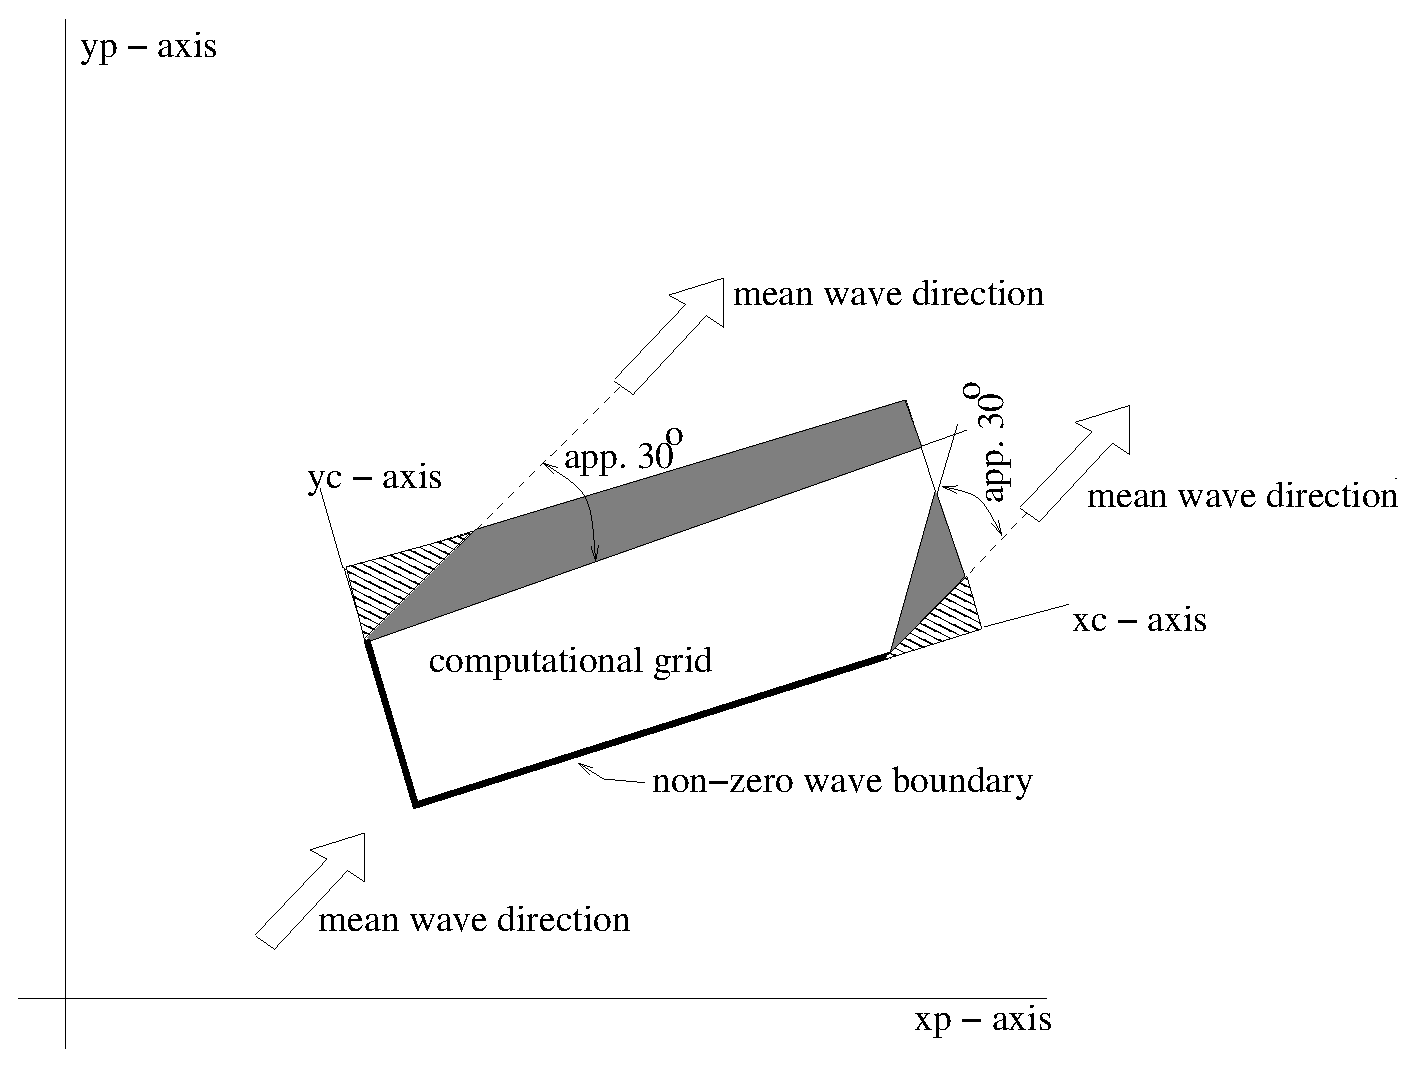
\epsfig{file=distureg.eps,height=8cm}
              }
   \caption{Disturbed regions in the computational grid due to erroneous boundary conditions are indicated
            with shaded areas.}
   \label{fig:boundreg}
\end{figure}

\noindent
When \underline{output} is requested along a \underline{boundary of the computational grid}, it may occur
that this output differs from the boundary conditions that are imposed by the user. The reason is that
SWAN accepts only the user-imposed \underline{incoming} wave components and that it replaces the user-imposed
\underline{outgoing} wave components with computed outgoing components (propagating to the boundary from
the interior region). The user is informed by means of a warning in the output when the
computed significant wave height differs more than 10\%, say (10\% is default), from the user-imposed
significant wave height (command {\tt BOUND}...). The actual value of this difference can be set by the
user (see the {\tt SET} command). Note that this warning will not apply in the case of unstructured grids.
\\[2ex]
\noindent
If the computational grid extends outside the input grid, the reader is referred to Section~\ref{sec:choigrd}
to find the assumptions of SWAN on depth, current, water level, wind, bottom friction in the non-overlapping area.
\\[2ex]
\noindent
The spatial resolution of the computational grid should be sufficient to resolve relevant details of the wave
field. Usually a good choice is to take the resolution of the computational grid approximately equal to that
of the bottom or current grid. If necessary, an unstructured grid may be used.
\\[2ex]
\noindent
SWAN may not use the entire user-provided computational grid if the user defines exception values on
the depth grid (see command {\tt INPGRID BOTTOM}) or on the curvi-linear computational grid (see command
{\tt CGRID}).
It must be noted that for parallel runs using MPI the user must indicate an exception value when
reading the bottom levels (by means of command {\tt INPGRID BOTTOM EXCEPTION}), in order to obtain
good load balancing.
\\[2ex]
\noindent
A computational grid point is either
\begin{itemize}
  \item \underline{wet}, i.e. the grid point is included in the computations since it represents water; this may vary
         with time-dependent or wave-induced water levels or
  \item \underline{dry}, i.e. the grid point is excluded from the computations since it represents land which may vary
        with time-dependent or wave-induced water levels or
  \item \underline{exceptional}, i.e. the grid point is permanently excluded from the computations since it is so
        defined by the user.
\end{itemize}
If \underline{exceptional grid points} occur in the computational grid, then SWAN filters the entire computational grid
as follows:
\begin{itemize}
  \item each grid line between two adjacent wet computational grid points (a wet link) \underline{without} an
        adjacent, parallel wet link, is removed,
  \item each wet computational grid point that is linked to only one other wet computational grid point,
        is removed and
  \item each wet computational grid point that has no wet links is removed.
\end{itemize}
The effect of this filter is that if exception values are used for the depth grid or the curvi-linear
computational grid, one-dimensional water features are ignored in the SWAN computations (results at
these locations with a width of about one grid step may be unrealistic). If no exception values are used,
the above described filter will not be applied. As a consequence, one-dimensional features may appear
or disappear due to changing water levels (flooding may create them, drying may reduce two-dimensional
features to one-dimensional features).
\\[2ex]
\noindent
The {\bf computational time window} must be defined by the user in case of nonstationary runs. The
computational window in time must start at a time that is early enough that the initial state of SWAN has
propagated through the computational area before reliable output of SWAN is expected. Before this time
the output may not be reliable since usually the initial state is not known and only either no waves or some
very young sea state is assumed for the initial state. This is very often erroneous and this erroneous initial
state is propagated into the computational area.
\\[2ex]
\noindent
The computational time step must be given by the user in case of nonstationary runs. Since, SWAN is
based on implicit numerical schemes, it is not limited by the Courant stability criterion (which couples
time and space steps). In this sense, the time step in SWAN is not restricted. However, the accuracy of
the results of SWAN are obviously affected by the time step. Generally, the time step in SWAN should be
small enough to resolve the time variations of computed wave field itself. Usually, it is enough to consider
the time variations of the driving fields (wind, currents, water depth, wave boundary conditions). But be
careful: relatively(!) small time variations in depth (e.g. by tide) can result in relatively(!) large
variations in the wave field.
\\[2ex]
\noindent
As default, the first guess conditions of a \underline{stationary} run of SWAN are determined with the
2$^{{\rm nd}}$ generation mode of SWAN. The initial condition of a \underline{nonstationary} run of SWAN
is by default a JONSWAP spectrum with a $\cos ^{2} (\theta )$ directional distribution centred around the
local wind direction.
\\[2ex]
\noindent
A quasi-stationary approach can be employed with stationary SWAN computations in a time-varying sequence
of stationary conditions.
\\[2ex]
\noindent
The {\bf computational spectral grid} needs to be provided by the user. In frequency space, it is simply
defined by a minimum and a maximum frequency and the frequency resolution which is proportional to
the frequency itself (i.e. logarithmic, e.g., $\Delta\, f\,\, =\,\, 0.1\,\, f$). The frequency domain may
be specified as follows (see command {\tt CGRID}):
\begin{itemize}
  \item The lowest frequency, the highest frequency and the number of frequencies can be chosen.
  \item Only the lowest frequency and the number of frequencies can be chosen. The highest frequency
        will be computed by SWAN such that $\Delta\, f\,\, =\,\, 0.1\,\, f$. This resolution is required
        by the DIA method for the approximation of nonlinear 4-wave interactions (the so-called quadruplets).
  \item Only the highest frequency and the number of frequencies can be chosen. The lowest frequency
        will be computed by SWAN such that $\Delta\, f\,\, =\,\, 0.1\,\, f$. This resolution is required by
        the DIA method for the approximation of nonlinear 4-wave interactions.
  \item Only the lowest frequency and the highest frequency can be chosen. The number of frequencies
        will be computed by SWAN such that $\Delta\, f\,\, =\,\, 0.1\,\, f$. This resolution is required
        by the DIA method for the approximation of nonlinear 4-wave interactions.
\end{itemize}
The value of lowest frequency must be somewhat smaller than 0.7 times the value of the lowest peak
frequency expected. The value of highest frequency must be at least 2.5 to 3 times the highest peak
frequency expected. For the XNL approach, however, this should be 6 times the highest peak frequency.
Usually, it is chosen less than or equal to 1 Hz.
\\[2ex]
\noindent
SWAN has the option to make computations that can be nested in WAM or WAVEWATCH~III. In such runs
SWAN interpolates the spectral grid of WAM or WAVEWATCH~III to the (user provided) spectral grid of
SWAN. The WAM Cycle 4 source term in SWAN has been retuned for a highest prognostic frequency (that
is explicitly computed by SWAN) of 1 Hz. It is therefore recommended that for cases where wind
generation is important and WAM Cycle 4 formulations are chosen, the highest prognostic frequency is
about 1 Hz.
\\[2ex]
\noindent
In directional space, the directional range is the full 360$^{{\rm o}}$ unless the user specifies a
limited directional range. This may be convenient (less computer time and/or memory space), for example,
when waves travel towards a coast within a limited sector of 180$^{{\rm o}}$. The directional resolution
is determined by the number of discrete directions that is provided by the user. For wind seas with a
directional spreading of typically 30$^{{\rm o}}$ on either side of the mean wave direction, a resolution
of 10$^{{\rm o}}$ seems enough whereas for swell with a directional spreading of less than 10$^{{\rm o}}$,
a resolution of 2$^{{\rm o}}$ or less may be required. If the user is confident that no energy will occur
outside a certain directional sector (or is willing to ignore this amount of energy), then the computations
by SWAN can be limited to the directional sector that does contain energy. This may often be the case of
waves propagating to shore within a sector of 180$^{{\rm o}}$ around some mean wave direction.
\\[2ex]
\noindent
It is recommended to use the following discretization in SWAN for applications in coastal areas:
\begin{table}[htb]
\begin{tabular}{l l}
\hline
   direction resolution for wind sea & $\Delta \theta = 15^o - 10^o$ \\
   direction resolution for swell    & $\Delta \theta = 5^o - 2^o$ \\
   frequency range                   & $0.04 \leq f \leq 1.00$ Hz \\
   spatial resolution                & $\Delta x, \Delta y = 50 - 1000$ m\\
\hline
\end{tabular}
\end{table}

\noindent
The numerical schemes in the SWAN model require a minimum number of discrete grid points in each
spatial directions of 2. The minimum number of directional bins is 3 per directional quadrant and
the minimum number of frequencies should be 4.

\subsection{Output grids}
SWAN can provide output on uniform, recti-linear spatial grids that are independent from the input grids
and from the computational grid. In the computation with a curvi-linear computational grid, curvi-linear
output grids are available in SWAN. This also holds for triangular meshes.
An output grid has to be specified by the user with an arbitrary
resolution, but it is of course wise to choose a resolution that is fine enough to show relevant spatial
details. It must be pointed out that the information on an output grid is obtained from the computational
grid by bi-linear interpolation (output always at computational time level). This implies that some
inaccuracies are introduced by this interpolation. It also implies that bottom or current information on an
output plot has been obtained by interpolating twice: once from the input grid to the computational grid
and once from the computational grid to the output grid. If the input-, computational- and output grids are
identical, then no interpolation errors occur.
\\[2ex]
\noindent
In the regions where the output grid does not cover the computational grid, SWAN assumes output values
equal to the corresponding exception value. For example, the default exception value for the significant
wave height is $-$9. The exception values of output quantities can be changed by means of the {\tt QUANTITY}
command.
\\[2ex]
\noindent
In nonstationary computations, output can be requested at regular intervals starting at a given time
always at computational times.

\section{Activation of physical processes}
SWAN contains a number of physical processes (see Scientific/Technical documentation) that add or withdraw wave energy to or
from the wave field. The processes included are: wind input, whitecapping, bottom friction, depth-induced
wave breaking,
dissipation due to vegetation,
obstacle transmission, nonlinear wave-wave interactions (quadruplets and triads) and
wave-induced set-up. SWAN can run in several modes, indicating the level of parameterization. SWAN can operate
in first-, second- and third-generation mode. The first- and second-generation modes are essentially those
of Holthuijsen and De Boer (1988); first-generation with a constant Phillips "constant" of 0.0081 and
second-generation with a variable Phillips "constant". An overview of the options is given in Table below.
\begin{table}[htb]
\begin{center}
\caption{Overview of physical processes and generation mode in SWAN.}
\label{tab:ovmod}
\begin{tabular}{|l | l | c | c | c|}
\hline
  \multicolumn{1}{|l|}{{\bf process}}&
  \multicolumn{1}{|l|}{{\bf authors}}&
  \multicolumn{3}{|l|}{{\bf generation}}\\
  \multicolumn{1}{|l|}{}&
  \multicolumn{1}{|l|}{}&
  \multicolumn{3}{|l|}{{\bf mode}}\\
\cline{3-5}
  \multicolumn{1}{|l|}{}&
  \multicolumn{1}{|l|}{}&
  \multicolumn{1}{|c|}{{\bf 1st}}&
  \multicolumn{1}{|c|}{{\bf 2nd}}&
  \multicolumn{1}{|c|}{{\bf 3rd}}\\
\hline
\hline
Linear wind growth      & Cavaleri and Malanotte-Rizzoli (1981)  & $\times$ & $\times$ &          \\
                        & (modified)                             &          &          &          \\
\cline{2-5}
                        & Cavaleri and Malanotte-Rizzoli (1981)  &          &          & $\times$ \\
\hline
Exponential wind growth & Snyder {\it et al}. (1981) (modified)  & $\times$ & $\times$ &          \\
\cline{2-5}
                        & Snyder {\it et al}. (1981)             &          &          & $\times$ \\
\cline{2-5}
                        & Janssen (1989, 1991)                   &          &          & $\times$ \\
\cline{2-5}
                        & Yan (1987) (modified)                  &          &          & $\times$ \\
\hline
Whitecapping            & Holthuijsen and De Boer (1988)         & $\times$ & $\times$ &          \\
\cline{2-5}
                        & Komen {\it et al}. (1984)              &          &          & $\times$ \\
\cline{2-5}
                        & Janssen (1991)                         &          &          & $\times$ \\
\cline{2-5}
                        & Alves and Banner (2003)                &          &          & $\times$ \\
\hline
Quadruplets             & Hasselmann {\it et al}. (1985)         &          &          & $\times$ \\
\hline
\hline
Triads                  & Eldeberky (1996)                       & $\times$ & $\times$ & $\times$ \\
\hline
Depth-induced breaking  & Battjes and Janssen (1978)             & $\times$ & $\times$ & $\times$ \\
\hline
Bottom friction         & JONSWAP (1973)                         & $\times$ & $\times$ & $\times$ \\
\cline{2-5}
                        & Collins (1972)                         & $\times$ & $\times$ & $\times$ \\
\cline{2-5}
                        & Madsen {\it et al}. (1988)             & $\times$ & $\times$ & $\times$ \\
\hline
Obstacle transmission   & Seelig (1979), d'Angremond (1996)      & $\times$ & $\times$ & $\times$ \\
\hline
Wave-induced set-up     &                                        & $\times$ & $\times$ & $\times$ \\
\hline
Vegetation dissipation  & Dalrymple (1984)                       & $\times$ & $\times$ & $\times$ \\
\hline
\end{tabular}
\end{center}
\end{table}
\noindent
The processes are activated as follows:
\begin{itemize}
  \item {\it Wind input} is activated by commands {\tt GEN1}, {\tt GEN2} or {\tt GEN3}\footnote{active by default, can be deactivated with command {\tt OFF}.}.
  \item {\it Whitecapping} is activated by commands {\tt GEN1}, {\tt GEN2} or {\tt GEN3}\footnote{active by default, can be deactivated with command {\tt OFF}.}.
  \item {\it Quadruplets} is activated by command {\tt GEN3}\footnote{active by default, can be deactivated with command {\tt OFF}.}.
  \item {\it Triads} is activated by command {\tt TRIAD}.
  \item {\it Bottom friction} is activated by command {\tt FRICTION}.
  \item {\it Depth-induced breaking} is activated by command {\tt BREAKING}\footnote{active by default, can be deactivated with command {\tt OFF}.}.
  \item {\it Vegetation dissipation} is activated by command {\tt VEGETATION}.
  \item {\it Obstacle transmission} is activated by command {\tt OBSTACLE}.
  \item {\it Wave-induced set-up} is activated by command {\tt SETUP}.
\end{itemize}
For the preliminary SWAN runs, it is strongly advised to use the default values of the model coefficients. First, it
should be determined whether or not a certain physical process is relevant to the result. If this cannot be
decided by means of a simple hand computation, one can perform a SWAN computation without and with
the physical process included in the computations, in the latter case using the standard values chosen
in SWAN.
\\[2ex]
\noindent
After it has been established that a certain physical process is important, it may be worthwhile to modify
coefficients. In the case of wind input one may at first try to vary the wind velocity. Concerning the bottom
friction, the best coefficients to vary are the friction coefficient. Switching off the depth-induced breaking
term is usually unwise, since this may lead to unacceptably high wave heights near beaches (the
computed wave heights 'explode' due to shoaling effects).

\section{Time and date notation}
SWAN can run for dates (i.e. nonstationary mode)
\begin{itemize}
  \item between the years 0 and 9999, if ISO-notation is used in the input (recommended) or
  \item between the years 1931 and 2030 if two-digit code for years is used (formats 2-6 in every
        command that contains moments in time).
\end{itemize}
Be careful when nesting SWAN in WAM, since WAM does not use ISO-notation.

\chap{Input and output files} \label{ch:inout}

\section{General}

SWAN is one single computer program. The names of the files provided by the user should comply with
the rules of file identification of the computer system on which SWAN is run. In addition: \underline{SWAN does not
permit file names longer than 36 characters}. Moreover, \underline{the maximum length of the lines in the input files
for SWAN is 120 positions}.
\\[2ex]
\noindent
The user should provide SWAN with a number of files (input files) with the following information:
\begin{itemize}
  \item a file containing the instructions of the user to SWAN (the command file),
  \item file(s) containing: grid, bottom, current, friction, and wind (if relevant) and
  \item file(s) containing the wave field at the model boundaries (if relevant).
\end{itemize}

\section{Input / output facilities}
To assist in making the command file, an edit file is available to the user (see Appendix~\ref{app:swanedt}). In its original
form this file consists only of comments; all lines begin with exclamation mark. In the file, all commands
as given in this User Manual (Chapter~\ref{ch:comm}) are reproduced as mnemonics for making the final command
file. Hence, the user does not need to consult the User Manual every time to check the correct spelling
of keywords, order of data, etc. The user is advised to first copy the edit file (the copy file should have a
different name) and then start typing commands between the comment lines of the edit file.
\\[2ex]
\noindent
SWAN is fairly flexible with respect to output processing. Output is available for many different wave
parameters and wave related parameters (e.g., wave-induced stresses and bottom orbital motion).
However, the general rule is that output is produced by SWAN only at the user's request. The instructions
of the user to control output are separated into three categories:
\begin{itemize}
  \item Definitions of the geographic location(s) of the output. The output locations may be either on a
        geographic grid, or along user specified lines (e.g., a given depth contour line) or at
        individual output locations.
  \item Times for which the output is requested (only in nonstationary runs).
  \item Type of output quantities (wave parameters, currents or related quantities).
\end{itemize}

\section{Print file and error messages}
\label{sec:prtfile}
SWAN always creates a print file. Usually the name of this file is identical to the name of the command
file of the computations with the extension (.SWN) replaced with (.PRT). Otherwise, it depends on the
batch file that is used by the user. Consult the Implementation Manual for more information.
\\[2ex]
\noindent
The print file contains an echo of the command file and error messages. These messages are usually
self-explanatory (if not, users may address the SWAN forum-page on the SWAN homepage). The print
file also contains computational results if the user so requests (with command {\tt BLOCK} or {\tt TABLE}).

\chap{Description of commands} \label{ch:comm}

\section{List of available commands} \label{sec:lstcomm}
The following commands are available to users of SWAN (to look for the commands quickly, see table of contents
and index).
\\[2ex]
\underline{\bf Start-up commands}
\begin{description}
  \item[(a)] Start-up commands:
\begin{tabbing}
xxxxxxxxxxxx\= \kill
{\tt PROJECT} \> title of the problem to be computed\\
{\tt SET}     \> sets values of certain general parameters\\
{\tt MODE}    \> requests a stationary / nonstationary or\+\\
                 1D-mode / 2D-mode of SWAN\-\\
{\tt COORD}   \> to choose between Cartesian and spherical coordinates\\
\end{tabbing}
\end{description}
\underline{\bf Commands for model description}
\begin{description}
  \item[(b)] Commands for computational grid:
\begin{tabbing}
xxxxxxxxxxxx\= \kill
{\tt CGRID}    \> defines dimensions of computational grid\\
{\tt READGRID} \> reads a \underline{curvi-linear} or \underline{unstructured} computational grid\\
\end{tabbing}
  \item[(c)] Commands for input fields:
\begin{tabbing}
xxxxxxxxxxxx\= \kill
{\tt INPGRID} \> defines dimensions of bottom, water level, current and friction grids\\
{\tt READINP} \> reads input fields\\
{\tt WIND}    \> activates constant wind option\\
\end{tabbing}
  \item[(d)] Commands for boundary and initial conditions:
\begin{tabbing}
xxxxxxxxxxxx\= \kill
{\tt BOUND}      \> defines the shape of the spectra at the boundary of geographic grid\\
{\tt BOUNDSPEC}  \> defines (parametric) spectra at the boundary of geographic grid\\
{\tt BOUNDNEST1} \> defines boundary conditions obtained from (coarse) SWAN run\\
{\tt BOUNDNEST2} \> defines boundary conditions obtained from WAM run\\
{\tt BOUNDNEST3} \> defines boundary conditions obtained from WAVEWATCH~III run\\
{\tt INITIAL}    \> specifies an initial wave field\\
\end{tabbing}
  \item[(e)] Commands for physics:
\begin{tabbing}
xxxxxxxxxxxx\= \kill
{\tt GEN1}     \> SWAN runs in first generation mode\\
{\tt GEN2}     \> SWAN runs in second generation mode\\
{\tt GEN3}     \> SWAN runs in third generation mode\\
{\tt QUAD}     \> controls the computation of quadruplets\\
{\tt BREAKING} \> activates dissipation by depth-induced wave breaking\\
{\tt FRICTION} \> activates dissipation by bottom friction\\
{\tt TRIAD}    \> activates three wave-wave interactions\\
{\tt VEGETAT}  \> activates dissipation due to vegetation\\
{\tt LIMITER}  \> de-actives quadruplets if a certain Ursell number exceeds\\
{\tt OBSTACLE} \> defines characteristics of sub-grid obstacles\\
{\tt SETUP}    \> activates the computation of the wave-induced set-up\\
{\tt DIFFRAC}  \> activates diffraction\\
{\tt OFF}      \> de-activates certain physical processes\\
\end{tabbing}
  \item[(f)] Commands for numerics:
\begin{tabbing}
xxxxxxxxxxxx\= \kill
{\tt PROP}    \> to choose the numerical propagation scheme\\
{\tt NUMERIC} \> sets some of the numerical properties of SWAN\\
\end{tabbing}
\end{description}
\underline{\bf Output commands}
\begin{description}
  \item[(g)] Commands for output locations:
\begin{tabbing}
xxxxxxxxxxxx\= \kill
{\tt FRAME}   \> defines an output frame (a regular grid)\\
{\tt GROUP}   \> defines an output group (for regular and curvi-linear grids)\\
{\tt CURVE}   \> defines an output curve\\
{\tt RAY}     \> defines a set of straight output lines (rays)\\
{\tt ISOLINE} \> defines a depth- or bottom contour (for output along that contour)\\
{\tt POINTS}  \> defines a set of individual output points\\
{\tt NGRID}   \> defines a nested grid\\
\end{tabbing}
  \item[(h)] Commands to write or plot output quantities:
\begin{tabbing}
xxxxxxxxxxxx\= \kill
{\tt QUANTITY} \> defines properties of output quantities\\
{\tt OUTPUT}   \> influence format of block, table and/or spectral output\\
{\tt BLOCK}    \> requests a block output (geographic distribution)\\
{\tt TABLE}    \> requests a table output (set of locations)\\
{\tt SPECOUT}  \> requests a spectral output\\
{\tt NESTOUT}  \> requests a spectral output for subsequent nested computations\\
\end{tabbing}
  \item[(i)] Commands to write or plot intermediate results:
\begin{tabbing}
xxxxxxxxxxxx\= \kill
{\tt TEST} \> requests an output of intermediate results for testing purposes\\
\end{tabbing}
\end{description}
\underline{\bf Lock-up commands}
\begin{description}
  \item[(j)] Commands to lock-up the input file:
\begin{tabbing}
xxxxxxxxxxxx\= \kill
{\tt COMPUTE} \> starts a computation\\
{\tt HOTFILE} \> stores results for subsequent SWAN run\\
{\tt STOP}    \> end of user's input\\
\end{tabbing}
\end{description}

\section{Sequence of commands} \label{sec:seqcomm}
SWAN executes the above command blocks (a,...,j) in the above sequence except (f), (i) and (j). The
commands of the blocks (f) and (i) may appear anywhere before block (j), except that {\tt TEST POINTS} must
come after {\tt READINP BOTTOM}. The commands of block (j) may appear anywhere in the command file (all
commands after {\tt COMPUTE} are ignored by SWAN, except {\tt HOTFILE} and {\tt STOP}). A sequence of
commands of block (g) is permitted (all commands will be executed without overriding). Also a sequence of
commands of block (h) is permitted (all commands will be executed without overriding).
\\[2ex]
\noindent
Within the blocks the following sequence is to be used:
\begin{tabbing}
xxxxxxxxxxxx\= \kill
{In block (a)} \>: no prescribed sequence in block\\
{In block (b)} \>: {\tt READGRID} after {\tt CGRID}\\
{In block (c)} \>: {\tt READINP} after {\tt INPGRID} (repeat both in this sequence for each quantity)\\
{In block (d)} \>: {\tt BOUND SHAPE} before {\tt BOUNDSPEC}, otherwise no prescribed sequence in block\\
{In block (e)} \>: use only one {\tt GEN} command; use command {\tt OFF} only after a {\tt GEN} command\+\\
                   (note that {\tt GEN3} is default)\-\\
{In block (f)} \>: no prescribed sequence in block\\
{In block (g)} \>: {\tt ISOLINE} after {\tt RAY} ({\tt ISOLINE} and {\tt RAY} can be repeated independently)\\
{In block (h)} \>: no prescribed sequence in block\\
{In block (i)} \>: no prescribed sequence in block\\
{In block (j)} \>: {\tt HOTFILE} immediately after {\tt COMPUTE}, {\tt STOP} after {\tt COMPUTE}\\
\end{tabbing}
It must be noted that a repetition of a command may override an earlier occurrence of that command.
\\[2ex]
\noindent
Many commands provide the user with the opportunity to assign values to coefficients of SWAN (e.g. the
bottom friction coefficient). If the user does not use such option SWAN will use a default value.
\\[2ex]
\noindent
Some commands cannot be used in 1D-mode (see individual command descriptions below).

\section{Command syntax and input / output limitations}

The command syntax is given in Appendix~\ref{app:syntax}.
\\[2ex]
\noindent
Limitations:
\begin{itemize}
  \item The maximum length of the input lines is 120 characters.
  \item The maximum length of the file names is 36 characters.
  \item The maximum length of the plot titles is 36 characters.
  \item The maximum number of file names is 99. This can be extended (edit the file {\tt swaninit} to change
        highest unit number of 99 to a higher number).
\end{itemize}

\section{Start-up} \label{sec:startup}

\idxcmd{PROJECT}
\linecmd
\begin{verbatim}
PROJect 'name' 'nr'

        'title1'

        'title2'

        'title3'
\end{verbatim}
\linecmd

\noindent
With this required command the user defines a number of strings to identify the SWAN run (project name
e.g., an engineering project) in the print and plot file.
\begin{tabbing}
xxxxxxxxxxxx\= \kill
{\tt 'name'}   \> is the name of the project, at most 16 characters long.\+\\
                  Default: blanks.\-\\
{\tt 'nr'}     \> is the run identification (to be provided as a character string; e.g. the run\+\\
                  number) to distinguish this run among other runs for the same project; it is at\\
                  most 4 characters long. It is the only required information in this command.\-\\
{\tt 'title1'} \> is a string of at most 72 characters provided by the user to appear in the\+\\
                  output of the program for the user's convenience.\\
                  Default: blanks.\-\\
{\tt 'title2'} \> same as {\tt 'title1'}.\\
{\tt 'title3'} \> same as {\tt 'title1'}.\\
\end{tabbing}

\idxcmd{SET}
\linecmd
\begin{verbatim}
SET  [level] [nor] [depmin] [maxmes] [maxerr] [grav] [rho] [cdcap]    &

                        |    NAUTical  |
     [inrhog] [hsrerr] <                > [pwtail] [froudmax] [printf] [prtest]
                        | -> CARTesian |
\end{verbatim}
\linecmd

\noindent
With this optional command the user assigns values to various general parameters.
\begin{tabbing}
xxxxxxxxxxxx\= \kill
{\tt [level]}   \> increase in water level that is constant in space and time can be given with\+\\
                   this option, {\tt [level]} is the value of this increase (in m). For a variable water\\
                   level reference is made to the commands {\tt INPGRID} and {\tt READINP}.\\
                   Default: {\tt [level]}=0.\-\\
{\tt [nor]}     \> direction of North with respect to the $x-$axis (measured counterclockwise);\+\\
                   default {\tt [nor]}= 90$^{{\rm o}}$, i.e. $x-$axis of the problem coordinate system\\
                   points East.\\
                   When spherical coordinates are used (see command {\tt COORD}) the value\\
                   of {\tt [nor]} may not be modified.\-\\
{\tt [depmin]}  \> threshold depth (in m). In the computation any positive depth smaller than\+\\
                   {\tt [depmin]} is made equal to {\tt [depmin]}.\\
                   Default: {\tt [depmin]} = 0.05.\-\\
{\tt [maxmes]}  \> maximum number of error messages (not necessarily the number of errors!)\+\\
                   during the computation at which the computation is terminated. During the\\
                   computational process messages are written to the print file.\\
                   Default: {\tt [maxmes]} = 200.\-\\
{\tt [maxerr]}  \> during pre-processing SWAN checks input data. Depending on the severity\+\\
                   of the errors encountered during this pre-processing, SWAN does not start\\
                   computations. The user can influence the error level above which SWAN will\\
                   not start computations (at the level indicated the computations will continue).\\
                   The error level {\tt [maxerr]} is coded as follows:\\
                   \pushtabs
                   xxx\=xxx \kill
                   1 \>: warnings,\\
                   2 \>: errors (possibly automatically repaired or repairable by SWAN),\\
                   3 \>: severe errors.\\
                   \poptabs
                   Default: {\tt [maxerr]} = 1.\-\\
{\tt [grav]}    \> is the gravitational acceleration (in m/s$^2$).\+\\
                   Default: {\tt [grav]} = 9.81.\-\\
{\tt [rho]}     \> is the water density $\rho$ (in kg/m$^3$).\+\\
                   Default: {\tt [rho]} = 1025.\-\\
{\tt [cdcap]}   \> is a maximum value for the wind drag coefficient. A value of {\tt [cdcap]} = 99999\+\\
                   means no cutting off the drag coefficient. A suggestion for this parameter is\\
                   {\tt [cdcap]} = 2.5$\times$ 10$^{-3}$.\\
                   Default: {\tt [cdcap]} = 99999.\-\\
{\tt [inrhog]}  \> to indicate whether the user requires output based on variance or based on true\+\\
                   energy (see Section~\ref{sec:units}).\\
                   \pushtabs
                   xxxxxxxxxxxxx\=xxx \kill
                   {\tt [inrhog]} = 0 \>: output based on variance\\
                   {\tt [inrhog]} = 1 \>: output based on true energy\\
                   \poptabs
                   Default: {\tt [inrhog]} = 0.\-\\
{\tt [hsrerr]}  \> the relative difference between the user imposed significant wave height and the\+\\
                   significant wave height computed by SWAN (anywhere along the computational\\
                   grid boundary) above which a warning will be given. This relative difference\\
                   is the difference normalized with the user provided significant wave height. This\\
                   warning will be given for each boundary grid point where the problem occurs\\
                   (with its $x-$ and $y-$index number of the computational grid). The cause of the\\
                   difference is explained in Section~\ref{sec:boundc}. To supress these warnings (in particular\\
                   for nonstationary computations), set {\tt [hsrerr]} at a very high value or use\\
                   command {\tt OFF BNDCHK}.\\
                   Default: {\tt [hsrerr]} = 0.10.\\
                   ONLY MEANT FOR STRUCTURED GRIDS.\-\\
{\tt NAUTICAL}  \> indicates that the Nautical convention for wind and wave direction (SWAN input\+\\
                   and output) will be used instead of the default Cartesian convention.\\
                   For definition, see Section~\ref{sec:units} or Appendix~\ref{app:defvar}.\-\\
{\tt CARTESIAN} \> indicates that the Cartesian convention for wind and wave direction (SWAN input\+\\
                   and output) will be used. For definition, see Section~\ref{sec:units} or Appendix~\ref{app:defvar}.\-\\
{\tt [pwtail]}  \> power of high frequency tail; defines the shape of the spectral tail above the\+\\
                   highest prognostic frequency {\tt [fhigh]} (see command {\tt CGRID}). The energy density\\
                   is assumed to be proportional to frequency to the power {\tt [pwtail]}.\\
                   Default values depend on formulations of physics:\\
                   \pushtabs
                   xxxxxxxxxxxxxxxxxxxxx\=xxx \kill
                   command {\tt GEN1}        \>: {\tt [pwtail]} = 5\\
                   command {\tt GEN2}        \>: {\tt [pwtail]} = 5\\
                   command {\tt GEN3 KOMEN}  \>: {\tt [pwtail]} = 4\\
                   command {\tt GEN3 JANSEN} \>: {\tt [pwtail]} = 5\\
                   \poptabs
                   If the user wishes to use another value, then this {\tt SET} command should be\\
                   located in the command file after the {\tt GEN1}, {\tt GEN 2} or {\tt GEN3} command\\
                   (these will override the {\tt SET} command with respect to {\tt [pwtail]}).\-\\
{\tt [froudmax]}\> is the maximum Froude number ($U/\sqrt{gd}$ with $U$ the current and $d$ the water\+\\
                   depth). The currents taken from a circulation model may mismatch with given\\
                   water depth $d$ in the sense that the Froude number becomes larger than 1.\\
                   For this, the current velocities will be maximized by Froude number times $\sqrt{gd}$.\\
                   Default: {\tt [froudmax]} = 0.8.\-\\
{\tt [printf]}  \> unit reference number of the {\tt PRINT} file. As default, {\tt [printf]} is equal to 4. If\+\\
                   it is changed to 6 all print output will be written to the screen. This is useful\\
                   if print output is lost due to abnormal end of the program, while information\\
                   about the reason is expected to be in the {\tt PRINT} file.\-\\
{\tt [prtest]}  \> unit reference number of the test output file. As default, {\tt [prtest]} is equal to 4.\+\\
                   If it is changed to 6 all test output will be written to the screen. This is\\
                   useful if test print output is lost due to abnormal end of the program, while\\
                   information about the reason is expected to be in the test output file.\-\\
\end{tabbing}

\idxcmd{MODE}
\linecmd
\begin{verbatim}
      |-> STATionary    |     |-> TWODimensional |
MODE <                   >   <                    >
      |   NONSTationary |     |   ONEDimensional |
\end{verbatim}
\linecmd

\noindent
With this optional command the user indicates that the run will be either stationary or nonstationary and
one-dimensional (1D-mode) or two-dimensional (2D-mode). Non-stationary means either (see command {\tt COMPUTE}):
\begin{description}
  \item[(a)] one nonstationary computations or
  \item[(b)] a sequence of stationary computations or
  \item[(c)] a mix of (a) and (b).
\end{description}
The default option is {\tt STATIONARY TWODIMENSIONAL}.

\idxcmd{COORDINATES}
\linecmd
\begin{verbatim}
             | -> CARTesian                 |
COORDINATES <                  | -> CCM |    > REPeating
             |    SPHErical   <          >  |
                               |  QC    |
\end{verbatim}
\linecmd

\noindent
Command to choose between Cartesian and spherical coordinates (see Section~\ref{sec:units}).
\\[2ex]
\noindent
A nested SWAN run must use the same coordinate system as the coarse grid SWAN run.
\begin{tabbing}
xxxxxxxxxxxx\= \kill
{\tt CARTESIAN} \> all locations and distances are in m. Coordinates are given with respect\+\\
                   to $x-$ and $y-$axes chosen by the user in the various commands.\-\\
{\tt SPHERICAL} \> all coordinates of locations and geographical grid sizes are given in degrees;\+\\
                   $x$ is longitude with $x=0$ being the Greenwich meridian and $x>0$ is East of\\
                   this meridian; $y$ is latitude with $y>0$ being the Northern hemisphere. Input\\
                   and output grids have to be oriented with their $x-$axis to the East; mesh sizes\\
                   are in degrees. All other distances are in meters.\-\\
{\tt CCM}       \> defines the projection method in case of spherical coordinates. CCM means\+\\
                   central conformal Mercator. The horizontal and vertical scales are uniform\\
                   in terms of cm/degree over the area shown. In the centre of the scale is\\
                   identical to that of the conventional Mercator projection (but only at that\\
                   centre). The area in the projection centre is therefore exactly conformal.\-\\
{\tt QC}        \> the projection method is quasi-cartesian, i.e. the horizontal and vertical scales\+\\
                   are equal to one another in terms of cm/degree.\-\\
{\tt REPEATING} \> this option is only for academic cases. It means that wave energy leaving at one\+\\
                   end of the domain (in computational $x-$direction) enter at the other side; it is\\
                   as if the wave field repeats itself in $x-$direction with the length of the domain\\
                   in $x-$direction.\\
                   This option cannot be used in combination with computation of set-up (see\\
                   command {\tt SETUP}). This option is available only with \underline{regular grids}.\-\\
\end{tabbing}
Note that spherical coordinates can also be used for relatively small areas, say 10 or 20 km horizontal
dimension. This may be useful if one obtains the boundary conditions by nesting in an oceanic model
which is naturally formulated in spherical coordinates.
\\[2ex]
\noindent
Note that in case of spherical coordinates regular grids must always be oriented E-W, N-S, i.e.
{\tt [alpc]}=0, {\tt [alpinp]}=0, {\tt [alpfr]}=0 (see commands {\tt CGRID}, {\tt INPUT GRID} and
{\tt FRAME}, respectively).


\section{Model description} \label{sec:moddesc}

\subsection{Computational grid}

\idxcmd{CGRID}
\linecmd
\begin{verbatim}
       | -> REGular [xpc] [ypc] [alpc] [xlenc] [ylenc] [mxc] [myc] |
       |                                                           |
CGRID <     CURVilinear [mxc] [myc]  (EXCeption  [xexc]  [yexc])    >  &
       |                                                           |
       |    UNSTRUCtured                                           |

          | -> CIRcle               |
         <                           > [mdc] [flow] [fhigh] [msc]
          |    SECtor [dir1] [dir2] |
\end{verbatim}
\linecmd

\noindent
With this required command the user defines the geographic location, size, resolution and orientation of
the \underline{computational grid} in the problem coordinate system (see Section~\ref{sec:boundc}) in
case of a \underline{uniform, recti-linear} computational grid, a \underline{curvi-linear} grid or
\underline{unstructured} mesh.
The origin of the regular grid and the direction of the positive $x-$axis of this grid
can be chosen arbitrary by the user. Must be used for nested runs. Note that in a nested case, the
geographic and spectral range (directional sector inclusive) and resolution may differ from the previous
run (outside these ranges zero's are used).
\begin{tabbing}
xxxxxxxxxxxx\= \kill
{\tt REGULAR}     \> this option indicates that the computational grid is to be taken as uniform and\+\\
                     rectangular.\-\\
{\tt CURVILINEAR} \> this option indicates that the computational grid is to be taken as curvi-linear.\+\\
                     The user must provide the coordinates of the grid points with command\\
                     {\tt READGRID COOR}.\-\\
{\tt UNSTRUCTURE} \> this option indicates that the computational grid is to be taken as unstructured.\+\\
                     The user must provide the coordinates of the vertices and the numbering of\\
                     triangles with the associated connectivity table with vertices with command\\
                     {\tt READGRID UNSTRUC}.\-\\
{\tt [xpc]}       \> geographic location of the origin of the computational grid in the problem\+\\
                     coordinate system ($x-$coordinate, in m). See command {\tt COORD}.\\
                     Default: {\tt [xpc]} = 0.0 (Cartesian coordinates).\\
                     In case of spherical coordinates there is no default, the user must give a value.\-\\
{\tt [ypc]}       \> geographic location of the origin of the computational grid in the problem\+\\
                     coordinate system ($y-$coordinate, in m). See command {\tt COORD}.\\
                     Default: {\tt [ypc]} = 0.0 (Cartesian coordinates).\\
                     In case of spherical coordinates there is no default, the user must give a value.\-\\
{\tt [alpc]}      \> direction of the positive $x-$axis of the computational grid (in degrees, Cartesian\+\\
                     convention). In 1D-mode, {\tt [alpc]} should be equal to the direction {\tt [alpinp]}\\
                     (see command {\tt INPGRID}).\\
                     Default: {\tt [alpc]} = 0.0.\-\\
{\tt [xlenc]}     \> length of the computational grid in $x-$direction (in m). In case of spherical\+\\
                     coordinates {\tt [xlenc]} is in degrees.\-\\
{\tt [ylenc]}     \> length of the computational grid in $y-$direction (in m). In 1D-mode, {\tt [ylenc]}\+\\
                     should be 0. In case of spherical coordinates {\tt [ylenc]} is in degrees.\-\\
{\tt [mxc]}       \> number of meshes in computational grid in $x-$direction for a uniform, recti-linear\+\\
                     grid or $\xi-$direction for a curvi-linear grid (this number is \underline{one less} than the\\
                     number of grid points in this domain!).\-\\
{\tt [myc]}       \> number of meshes in computational grid in $y-$direction for a uniform, recti-linear\+\\
                     grid or $\eta-$direction for a curvi-linear grid (this number is \underline{one less} than the\\
                     number of grid points in this domain!). In 1D-mode, {\tt [myc]} should be 0.\-\\
{\tt EXCEPTION}   \> only available in the case of a \underline{curvi-linear grid}. If certain grid points are to be\+\\
                     ignored during the computation (e.g. land points that remain dry i.e. no\\
                     flooding; saving computer time and memory), then this can be indicated by\\
                     identifying these grid points in the file containing the grid point coordinates\\
                     (see command {\tt READGRID}). For an alternative, see command {\tt INPGRID BOTTOM}.\-\\
{\tt [xexc]}      \> the value which the user uses to indicate that a grid point is to be ignored\+\\
                     in the computations (this value is provided by the user at the location of the\\
                     $x-$coordinate considered in the file of the $x-$coordinates, see command\\
                     {\tt READGRID COOR}). Required if this option {\tt EXCEPTION} is used.\\
                     Default: {\tt [xexc]} = 0.0.\-\\
{\tt [yexc]}      \> the value which the user uses to indicate that a grid point is to be ignored\+\\
                     in the computations (this value is provided by the user at the location of the\\
                     $y-$coordinate considered in the file of the $y-$coordinates, see command\\
                     {\tt READGRID COOR}). Required if this option {\tt EXCEPTION} is used.\\
                     Default: {\tt [yexc]} = {\tt [xexc]}.\-\\
{\tt CIRCLE}      \> this option indicates that the spectral directions cover the full circle.\+\\
                     This option is default.\-\\
{\tt SECTOR}      \> this option means that only spectral wave directions in a limited directional sector\+\\
                     are considered; the range of this sector is given by {\tt [dir1]} and {\tt [dir2]}.\-\\
                  \> It must be noted that if the quadruplet interactions are to be computed (see\+\\
                     command {\tt GEN3}), then the {\tt SECTOR} should be 30$^o$ wider on each side than the\\
                     directional sector occupied by the spectrum (everywhere in the computational grid).\\
                     If not, then these computations are inaccurate. If the directional distribution of the\\
                     spectrum is symmetric around the centre of the {\tt SECTOR}, then the computed\\
                     quadruplet wave-wave interactions are effectively zero in the 30$^o$ range on\\
                     either end of the {\tt SECTOR}. The problem can be avoided by not activating\\
                     the quadruplet wave-wave interactions (use command {\tt GEN1} or {\tt GEN2}) or, if\\
                     activated (with command {\tt GEN3}), by subsequently de-activating them with\\
                     command {\tt OFF QUAD}.\-\\
{\tt [dir1]}      \> the direction of the right-hand boundary of the sector when looking outward from\+\\
                     the sector (required for option {\tt SECTOR}) in degrees.\-\\
{\tt [dir2]}      \> the direction of the left-hand boundary of the sector when looking outward from\+\\
                     the sector (required for option {\tt SECTOR}) in degrees.\-\\
{\tt [mdc]}       \> number of meshes in $\theta-$space. In the case of {\tt CIRCLE}, this is the number of\+\\
                     subdivisions of the 360 degrees of a circle, so $\Delta\theta$ = [360$^o$]/{\tt [mdc]} is the spectral\\
                     directional resolution. In the case of {\tt SECTOR}, $\Delta\theta$ = ({\tt [dir2]} - {\tt [dir1]})/{\tt [mdc]}.\\
                     The minimum number of directional bins is 3 per directional quadrant.\-\\
{\tt [flow]}      \> lowest discrete frequency that is used in the calculation (in Hz).\\
{\tt [fhigh]}     \> highest discrete frequency that is used in the calculation (in Hz).\\
{\tt [msc]}       \> \underline{one less} than the number of frequencies. This defines the grid resolution\+\\
                     in frequency-space between the lowest discrete frequency {\tt [flow]} and the highest\\
                     discrete frequency {\tt [fhigh]}. This resolution is not constant, since the frequencies\\
                     are distributed logarithmical: $f_{i+1} = \gamma f_i$ with $\gamma$ is a constant. The minimum\\
                     number of frequencies is 4.\\
                     The value of {\tt [msc]} depends on the frequency resolution $\Delta f$ that the user requires.\\
                     Since, the frequency distribution on the frequency axis is logarithmic, the\\
                     relationship is:\\
                     \\
                     $\Delta f = \left( -1 + \left[ {\frac{\mbox{\tt [fhigh]}}{\mbox{\tt [flow]}}} \right] ^{1/{\mbox{\tt [msc]}}} \right)f$\\
                     \\
                     Vice versa, if the user chooses the value of $\Delta f/f \,\,(=\gamma-1.)$, then the value of\\
                     {\tt [msc]} is given by:\\
                     \\
                     $\mbox{\tt [msc]} = \log (\mbox{\tt [fhigh]}/\mbox{\tt [flow]})/\log (1+\Delta f/f)$\\
                     \\
                     In this respect, it must be observed that the DIA approximation of the quadruplet\\
                     interactions (see command {\tt GEN3}) is based on a frequency resolution of $\Delta f/f = 0.1$\\
                     and hence, $\gamma = 1.1$. The actual resolution in the computations should therefore\\
                     not deviate too much from this. Alternatively, the user may only specifies one of\\
                     the following possibilities:\\
                     \pushtabs
                     xxxx\=xxx \kill
                     {$\bullet$} \> {\tt [flow]} and {\tt [msc]}; SWAN will compute {\tt [fhigh]}, such that $\gamma=1.1$,\+\\
                                    and write it to the {\tt PRINT} file.\-\\
                     {$\bullet$} \> {\tt [fhigh]} and {\tt [msc]}; SWAN will compute {\tt [flow]}, such that $\gamma=1.1$,\+\\
                                    and write it to the {\tt PRINT} file.\-\\
                     {$\bullet$} \> {\tt [flow]} and {\tt [fhigh]}; SWAN will compute {\tt [msc]}, such that $\gamma=1.1$,\+\\
                                    and write it to the {\tt PRINT} file.\-\\
                     \poptabs
\end{tabbing}
For illustration of a regular grid with its dimensions, see Figure~\ref{fig:compdom}.
\begin{figure}[htp]
   \centerline{
      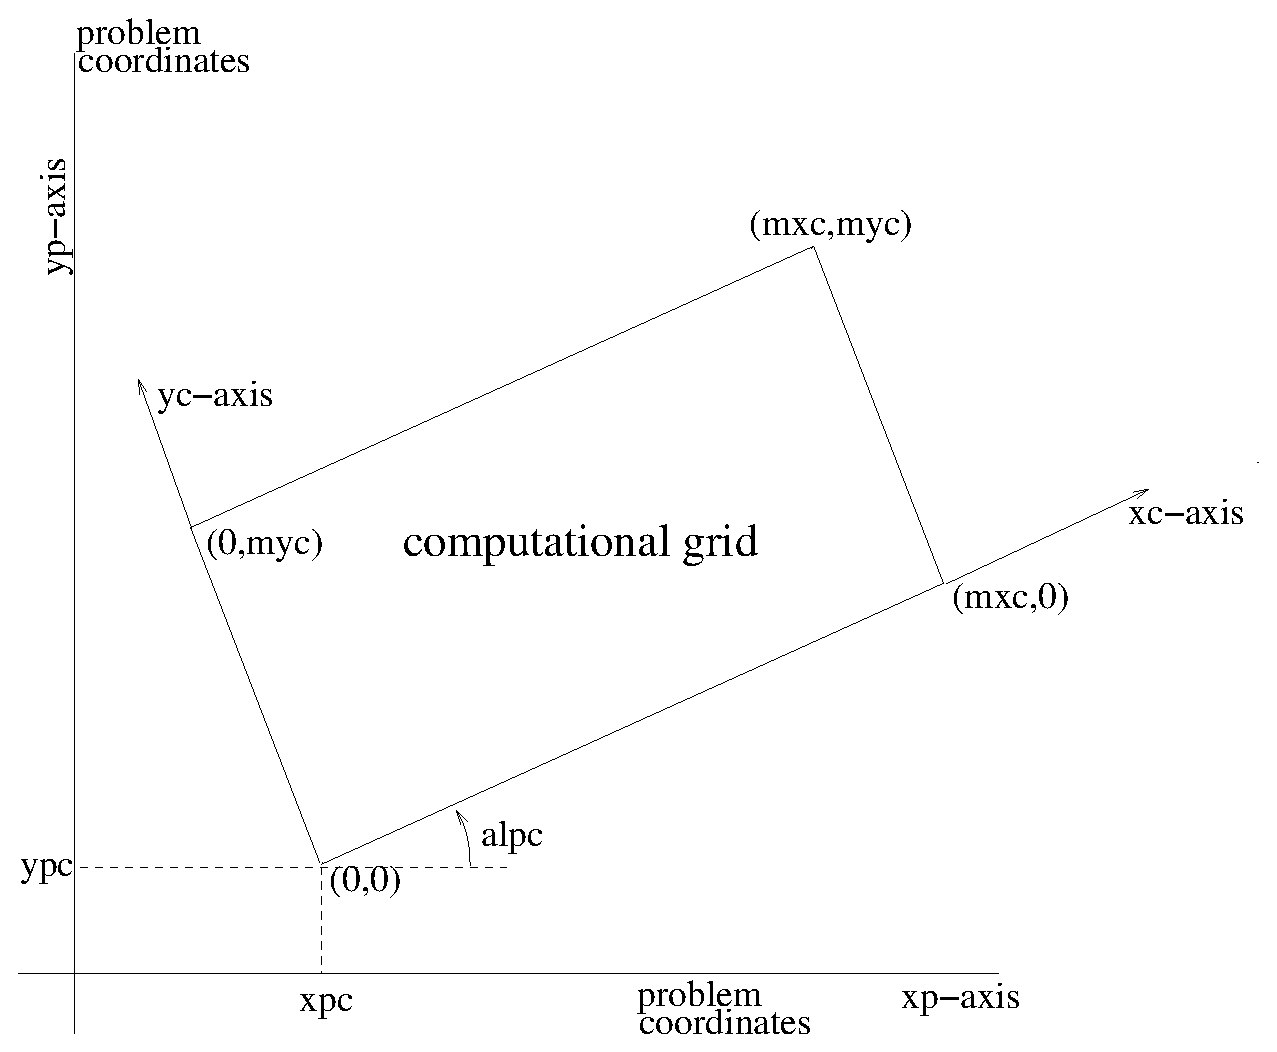
\epsfig{file=swangrid.eps,height=8cm}
              }
   \caption{Coordinates of the origin {\tt [xpc]} and {\tt [ypc]}, the orientation {\tt [alpc]} and the grid point
            numbering of the computational grid with respect to the problem coordinates system. Note that in case of
            spherical coordinates the $xc-$ and $xp-$axes both point East.}
   \label{fig:compdom}
\end{figure}

\idxcmd{READGRID COORDINATES}
\linecmd
\begin{verbatim}
READgrid COORdinates [fac] 'fname' [idla] [nhedf] [nhedvec] &

                           | -> FREe                 |
                           |                         |
                           |             | 'form' |  |
                          <     FORmat  <          >  >
                           |             | [idfm] |  |
                           |                         |
                           |    UNFormatted          |
\end{verbatim}
\linecmd

\noindent
CANNOT BE USED IN \underline{1D-MODE}.
\\[2ex]
\noindent
\underline{This command {\tt READGRID COOR} must follow a command {\tt CGRID CURV}}.
With this command (required if the computational grid is \underline{curvi-linear}; not allowed in case of a regular grid) the
user controls the reading of the co-ordinates of the computational grid points. These co-ordinates must
be read from a file as a vector ($x-$coordinate, $y-$coordinate of each single grid point).
See command {\tt READINP} for the description of the options in this command {\tt READGRID}.
SWAN will check whether all angles in the grid are $>0$ and $<180$ degrees. If not, it will print
an error message giving the coordinates of the grid points involved. It is recommended to use grids with
angles between 45 and 135 degrees.

\idxcmd{READGRID UNSTRUCTURED}
\linecmd
\begin{verbatim}
                        | -> ADCirc
                        |
READgrid UNSTRUCtured  <     TRIAngle |
                        |              > 'fname'
                        |    EASYmesh |
\end{verbatim}
\linecmd

\noindent
CANNOT BE USED IN \underline{1D-MODE}.
\\[2ex]
\noindent
\underline{This command {\tt READGRID UNSTRUC} must follow a command {\tt CGRID UNSTRUC}}.
With this command (required if the computational grid is \underline{unstructured}; not allowed in case of a regular or
curvi-linear grid) the user controls the reading of the ($x,y$) co-ordinates of the vertices including boundary markers and
a connectivity table for triangles (or elements). This table contains three corner vertices around each triangle in counterclockwise order.
This information should be provided by a number of files generated by one of the following grid generators currently supported by SWAN:
\begin{itemize}
  \item ADCIRC (\hl{http://www.adcirc.org})
  \item Triangle (\hl{http://www.cs.cmu.edu/afs/cs/project/quake/public/www/triangle.html})
  \item Easymesh (\hl{http://www-dinma.univ.trieste.it/nirftc/research/easymesh/easymesh.html})
\end{itemize}
After setting up the vertices and the connectivity tables for cells and faces (automatically done in SWAN), SWAN will print
some information concerning the used mesh, among others, number of vertices, cells and faces and minimum and maximum gridsizes.
Furthermore, SWAN will check at two levels for a possible occurence of badly shaped triangles. Firstly, the number of triangles that meet at each
vertex inside the mesh should not be smaller than 4 or larger than 10. Secondly, the angles inside each triangle should not be higher
than 143$^o$. If, at least, one of these two situations occur, SWAN will print an error message.
\begin{tabbing}
xxxxxxxxxxx\= \kill
{\tt ADCIRC}   \> the necessary grid information is read from file {\tt fort.14} as used by ADCIRC.\+\\
                  This file also contains the depth information that is read as well.\-\\
{\tt TRIANGLE} \> the necessary grid information is read from two files as produced by Triangle.\+\\
                  The {\tt .node} and {\tt .ele} files are required. The basename of these files must be\\
                  indicated with parameter {\tt 'fname'}.\-\\
{\tt EASYMESH} \> the necessary grid information is read from two files as produced by\+\\
                  Easymesh. The {\tt .n} and {\tt .e} files are required. The basename of these files\\
                  must be indicated with parameter {\tt 'fname'}.\-\\
{\tt 'fname'}  \> basename of the required files, i.e. without extension. Only meant for\+\\
                  Triangle and Easymesh.\-\\
\end{tabbing}

\subsection{Input grids and data}

\idxcmd{INPGRID}
\linecmd
\begin{verbatim}
              | BOTtom      |
              |             |
              | WLEVel      |
              |             |
              |  | CURrent  |
              | <           |
              |  | VX       |
              |  | VY       |
              |             |
INPgrid     (<               >)                                                 &
              | FRiction    |
              |             |
              |  | WInd     |
              | <           |
              |  | WX       |
              |  | WY       |
              |             |
              | NPLAnts     |

       | -> REGular [xpinp] [ypinp] [alpinp] [mxinp] [myinp] [dxinp] [dyinp] |
       |                                                                     |
      <     CURVilinear  [stagrx] [stagry] [mxinp] [myinp]                    > &
       |                                                                     |
       |    UNSTRUCtured                                                     |

        (EXCeption  [excval])                                                   &

                                            | -> Sec  |
        (NONSTATionary [tbeginp] [deltinp] <     MIn   >  [tendinp])
                                            |    HR   |
                                            |    DAy  |

\end{verbatim}
\linecmd

\noindent
OPTIONS \underline{CURVILINEAR} AND \underline{UNSTRUCTURED} NOT FOR \underline{1D-MODE}.
\\[2ex]
\noindent
With this required command the user defines the geographic location, size and orientation of an input grid
and also the time characteristics of the variable if it is not stationary. If this is the case (the variable is not
stationary), the variable should be given in a sequence of fields, one for each time step {\tt [deltinp]}. The
actual reading of values of bottom levels, currents, etc. from file is controlled by the command {\tt READINP}.
\underline{This command {\tt INPGRID} must precede the following command {\tt READINP}}.
\\[2ex]
\noindent
There can be different grids for bottom level ({\tt BOTTOM}), flow current ({\tt CURRENT}), bottom friction coefficient
({\tt FRICTION}), wind velocity ({\tt WIND}) and vegetation density ({\tt NPLANTS}).
If the current velocity components are available on different grids,
then option {\tt VX}, {\tt VY} can define these different grids for the $x-$ and $y-$component of the current, respectively
(but the grids must have identical orientation). Different grids for {\tt VX} and {\tt VY} may be useful if the data are
generated by a circulation model using a staggered grid. The same holds for the wind velocity
components. \underline{If the command {\tt INPGRID} is given without any of the keywords {\tt BOTTOM}, {\tt WIND}, etc.}
\underline{it is assumed that all the input grids are the same}.
\\[2ex]
\noindent
In the case of a regular grid (option {\tt REGULAR} in the {\tt INPGRID} command) the current and wind vectors
are defined with the $x-$ and $y-$component of the current or wind vector with respect to the \underline{$x-$axis of the input
grid}. In case of a curvi-linear grid (option {\tt CURVILINEAR} in the {\tt INPGRID} command) the current and wind
vectors are defined with the $x-$ and $y-$component of the current or wind vector with respect to the \underline{$x-$axis of
the problem} \underline{coordinate system}. For wind velocity and friction coefficient it is also possible to use a
constant value over the computational field (see commands {\tt WIND} and {\tt FRICTION}). No grid definition for
wind and friction is then required.
\\[2ex]
\noindent
Note that in case of option {\tt BOTTOM} only stationary input field is allowed.
\\[2ex]
\noindent
Note that in 1D mode, both $x-$ and $y-$components of the current and/or wind must be specified. Also, {\tt VX} and {\tt WX}
must always be followed by {\tt VY} and {\tt WY}, respectively.
\\[2ex]
\noindent
If the computational grid is unstructured (generated by Triangle or Easymesh), the input grids can be either regular
or identical to the used computational grid.
\\[2ex]
\noindent
Do not use the command {\tt INP BOTTOM} when the unstructured grid of ADCIRC is employed!
The file {\tt fort.14} contains the bottom levels and will be read by SWAN through the command {\tt READ UNSTRUC ADCIRC}.
\\[2ex]
\noindent
If land points remain dry during the computation (no flooding!), then these points can be ignored.
In this way, turn-around time and internal memory can be saved. This can be done by indicating bottom level in these points as
exception value. See command {\tt INPGRID BOTTOM EXCEPTION}.
\\[2ex]
\noindent
For parallel runs using MPI, an exception value for bottom levels should be prescribed in order
to have a good load-balancing!
\\[2ex]
\noindent
See Section~\ref{sec:choigrd} for more information on grids.
\begin{tabbing}
xxxxxxxxxxxx\= \kill
{\tt BOTTOM}        \> defines the input grid of the bottom level. (For the definition of the bottom\+\\
                       level, see command {\tt READINP}).\-\\
{\tt WLEV}          \> water level relative to datum level, positive upward (in m).\\
{\tt CURRENT}       \> defines the input grid of the current field (same grid for $x-$ and $y-$components).\\
{\tt VX}            \> defines the input grid of the $x-$component of the current field (different grid\+\\
                       than $y-$component but same orientation).\-\\
{\tt VY}            \> defines input grid of the $y-$component of the current field (different grid than\+\\
                       $x-$component but same orientation).\-\\
{\tt FRICTION}      \> defines input grid of the bottom friction coefficient (defined in command\+\\
                       {\tt FRICTION}, not to be confused with this option {\tt FRICTION}!).\-\\
{\tt WIND}          \> defines input grid of the wind field (same grid for $x-$ and $y-$component).\+\\
                       If neither of the commands {\tt WIND} and {\tt READINP WIND} is used it is\\
                       assumed that there is no wind.\-\\
{\tt WX}            \> defines input grid of the $x-$component of the wind field (different grid than\+\\
                       $$x-$$component but same orientation).\-\\
{\tt WY}            \> defines input grid of the $y-$component of the wind field (different grid than\+\\
                       $y-$component but same orientation).\-\\
{\tt NPLANTS}       \> defines input grid of the horizontally varying vegetation density (defined\+\\
                       in command {\tt VEGETATION}).\-\\
{\tt REGULAR}       \> means that the input grid is uniform and rectangular.\\
{\tt CURVILINEAR}   \> means that the input grid is curvi-linear; this option is available only if the\+\\
                       computational grid is curvi-linear as well. The input grid is identical\\
                       (which is default) to the computational grid, or it is staggered in $x-$ and/or\\
                       $y-$direction.\\
                       NOT FOR \underline{1D-MODE}.\-\\
{\tt UNSTRUCTURE}   \> means that the input grid is unstructured; this option is available only if the\+\\
                       computational grid is unstructured as well. The input grid must be identical\\
                       to the computational grid.\\
                       NOT FOR \underline{1D-MODE}.\-\\
\end{tabbing}
For a {\tt REGULAR} grid:
\begin{tabbing}
xxxxxxxxxxxx\= \kill
{\tt [xpinp]}       \> geographic location ($x-$coordinate) of the origin of the input grid in\+\\
                       \underline{problem coordinates} (in m) if Cartesian coordinates are used or in degrees if\\
                       spherical coordinates are use (see command {\tt COORD}).\\
                       Default: {\tt [xpinp]} = 0. In case of spherical coordinates there is no default, the\\
                       user must give a value.\-\\
{\tt [ypinp]}       \> geographic location ($y-$coordinate) of the origin of the input grid in\+\\
                       \underline{problem coordinates} (in m) if Cartesian coordinates are used or in degrees if\\
                       spherical coordinates are use (see command {\tt COORD}).\\
                       Default: {\tt [ypinp]} = 0. In case of spherical coordinates there is no default, the\\
                       user must give a value.\-\\
{\tt [alpinp]}      \> direction of the positive $x-$axis of the input grid (in degrees, Cartesian convention).\+\\
                       See command {\tt COORD}.\\
                       Default: {\tt [alpinp]} = 0.\-\\
{\tt [mxinp]}       \> number of meshes in $x-$direction of the input grid (this number is \underline{one less}\+\\
                       than the number of grid points in this direction!).\-\\
{\tt [myinp]}       \> number of meshes in $y-$direction of the input grid (this number is \underline{one less}\+\\
                       than the number of grid points in this direction!).\\
                       In \underline{1D-mode}, {\tt [myinp]} should be 0.\-\\
{\tt [dxinp]}       \> mesh size in $x-$direction of the input grid,\+\\
                       in m in case of Cartesian coordinates or\\
                       in degrees if spherical coordinates are used, see command {\tt COORD}.\-\\
{\tt [dyinp]}       \> mesh size in $y-$direction of the input grid,\+\\
                       in m in case of Cartesian coordinates or\\
                       in degrees if spherical coordinates are used, see command {\tt COORD}.\\
                       In \underline{1D-mode}, {\tt [dyinp]} may have any value.\\
                       Default: {\tt [dyinp]} = {\tt [dxinp]}.\-\\
\end{tabbing}
For a {\tt CURVILINEAR} input (not fully tested for spherical coordinates):
\begin{tabbing}
xxxxxxxxxxxx\= \kill
{\tt [mxinp]}       \> number of meshes in $\xi-$direction of the input grid (this number is \underline{one less}\+\\
                       than the number of grid points in this direction!).\\
                       Default: {\tt [mxinp]} = {\tt [mxc]}.\-\\
{\tt [myinp]}       \> number of meshes in $\eta-$direction of the input grid (this number is \underline{one less}\+\\
                       than the number of grid points in this direction!).\\
                       Default: {\tt [myinp]} = {\tt [myc]}.\-\\
{\tt [stagrx]}      \> staggered $x'-$direction with respect to computational grid; default: 0.\+\\
                       Note: e.g. {\tt [stagrx]}=0.5 means that the input grid points are shifted a half\\
                       step in $x'-$direction; in many flow models $x-$velocities are defined in points\\
                       shifted a half step in $x'-$direction.\-\\
{\tt [stagry]}      \> staggered $y'-$direction with respect to computational grid; default: 0.\+\\
                       Note: e.g. {\tt [stagry]}=0.5 means that the input grid points are shifted a half\\
                       step in $y'-$direction; in many flow models $y-$velocities are defined in points\\
                       shifted a half step in $y'-$direction.\-\\
{\tt EXCEPTION}     \> certain points inside the given grid that are to be ignored during the\+\\
                       computation can be identified by means of an exception value as given in\\
                       the corresponding input file as controlled by the command {\tt READINP}.\\
                       NOT FOR \underline{1D-MODE}.\-\\
{\tt [excval]}      \> exception value; required if the option {\tt EXCEPTION} is used.\+\\
                       Note: if {\tt [fac]} $\neq$ 1 (see command {\tt READINP}), {\tt [excval]} must be given as\\
                       {\tt [fac]} times the exception value.\-\\
{\tt NONSTATION}    \> the variable is nonstationary (given in a time sequence of fields).\+\\
                       NOT FOR \underline{1D-MODE}.\-\\
{\tt [tbeginp]}     \> begin time of the first field of the variable, the format is:\+\\
                       \pushtabs
                       xx\=xxxxxxxxxxxxxxxxxxxxxx\=xxxxxxxxxxxxx \kill
                       1 \>: ISO-notation           \> 19870530.153000          \\
                       2 \>: (as in HP compiler)    \> '30$-$May$-$87 15:30:00' \\
                       3 \>: (as in Lahey compiler) \> 05/30/87.15:30:00        \\
                       4 \>:                        \> 15:30:00                 \\
                       5 \>:                        \> 87/05/30 15:30:00'       \\
                       6 \>: as in WAM              \> 8705301530               \\
                       \poptabs
                       This format is installation dependent. See Implementation Manual or ask the\\
                       person who installed SWAN on your computer. Default is ISO-notation.\-\\
{\tt [deltinp]}     \> time interval between fields, the unit is indicated in the next option:\+\\
                       \pushtabs
                       xxxxxxx\=xxxxxxxxxxxxx \kill
                       SEC \> unit seconds\\
                       MIN \> unit minutes\\
                       HR  \> unit hours\\
                       DAY \> unit days\-\\
                       \poptabs
{\tt [tendinp]}     \> end time of the last field of the variable, the format is:\+\\
                       \pushtabs
                       xx\=xxxxxxxxxxxxxxxxxxxxxx\=xxxxxxxxxxxxx \kill
                       1 \>: ISO-notation           \> 19870530.153000          \\
                       2 \>: (as in HP compiler)    \> '30$-$May$-$87 15:30:00' \\
                       3 \>: (as in Lahey compiler) \> 05/30/87.15:30:00        \\
                       4 \>:                        \> 15:30:00                 \\
                       5 \>:                        \> 87/05/30 15:30:00'       \\
                       6 \>: as in WAM              \> 8705301530               \\
                       \poptabs
                       This format is installation dependent. See Implementation Manual or ask the\\
                       person who installed SWAN on your computer. Default is ISO-notation.\-\\
\end{tabbing}

\idxcmd{READINP}
\linecmd
\begin{verbatim}
          |  BOTtom      |
          |              |
          |  WLEVel      |
          |              |
          |  CURrent     |
          |              |           |  'fname1'            |
READinp  <   WInd         >  [fac]  <                        >   [idla]    &
          |              |           |  SERIes   'fname2'   |
          |  FRiction    |
          |              |
          |  NPLAnts     |

                                           | -> FREe                       |
                                           |                               |
                                           |                 | 'form' |    |
           [nhedf] ([nhedt]) ([nhedvec])  <     FORmat      <          >    >
                                           |                 | [idfm] |    |
                                           |                               |
                                           |    UNFormatted                |
\end{verbatim}
\linecmd

\noindent
With this required command the user controls the reading of values of the indicated variables from file.
\underline{This command {\tt READINP} must follow a command {\tt INPGRID}}. Note that for each stationary or nonstationary
field, one combination of {\tt INPGRID} and {\tt READINP} suffices if one has more than one {\tt COMPUTE} command in a run.
\\[2ex]
\noindent
If the variables are in one file, then the {\tt READINP} commands should be given in the same sequence as the sequence in
which the variables appear in the file.
\begin{tabbing}
xxxxxxxxxxxx\= \kill
{\tt BOTTOM}        \> with this option the user indicates that bottom levels (m) are to be read from\+\\
                       file (bottom level positive downward relative to an arbitrary horizontal datum\\
                       level). The sign of the input can be changed with option {\tt [fac]} = $-1$. (see below).\-\\
{\tt WLEV}          \> with this option the user indicates that water levels (m) are to be read from\+\\
                       file (water level positive upward relative to the same datum level as used in\\
                       option {\tt BOTTOM}). Sign of input can be changed with option {\tt [fac]} = $-1$. If the\\
                       water level is constant in space and time, the user can use the command {\tt SET}\\
                       to add this water level to the water depth.\-\\
{\tt CURRENT}       \> recti-linear (curvi-linear) input grid: with this option the user indicates that\+\\
                       the $x-$ and $y-$component ($\xi-$ and $\eta-$component) are to be read from one and\\
                       the same file (with one {\tt READINP} command). With this option SWAN reads first all\\
                       $x-$components ($\xi-$components), and then all $y-$components ($\eta-$components)\\
                       (see below). The firs component ($x-$ or $\xi-$component) is always eastward oriented\\
                       and the second one ($y-$ or $\eta-$component) is always northwise oriented. The\\
                       components  $\xi$ and $\eta$ are taken along the directions of the grid lines\\
                       of the curvi-linear grid! If the current velocity is relatively large, i.e.\\
                       the Froude number $U/ \sqrt{g d}$ is larger than 0.8, it will be reduced such that\\
                       the Froude number becomes equal to 0.8.\-\\
{\tt WIND}          \> recti-linear (curvi-linear) input grid: with this option the user indicates that\+\\
                       the $x-$ and $y-$component ($\xi-$ and $\eta-$component) are to be read from one and\\
                       the same file (with one {\tt READINP} command). With this option SWAN reads first\\
                       all $x-$components ($\xi-$components), and then all $y-$component ($\eta-$components)\\
                       (see below). The components $\xi$ and $\eta$  are taken along the directions of the grid\\
                       lines of the curvi-linear grid! If the wind is constant, see command {\tt WIND}.\-\\
{\tt FRICTION}      \> with this option the user indicates that friction coefficient is to be read from\+\\
                       file for Collins: {\tt [cfw]} and for Madsen: {\tt [kn]} (no space- or time-variable\\
                       coefficient for the Jonswap expression, see command {\tt FRICTION}). If the\\
                       coefficients are constant in space and time: see command {\tt FRICTION}.\-\\
{\tt NPLANTS}       \> with this option the user indicates that horizontally varying vegetation\+\\
                       density (per m$^2$) is to be read from file. If the density is constant then\\
                       see command {\tt VEGETATION} for specifcation.\-\\
{\tt [fac]}         \> SWAN multiplies all values that are read from file with {\tt [fac]}. For instance\+\\
                       if the bottom levels are given in unit decimeter, one should make {\tt [fac]}=0.1 to\\
                       obtain levels in m. To change sign of bottom level use a negative value of {\tt [fac]}.\\
                       Note that {\tt [fac]} = 0 is not allowed!\\
                       Default: {\tt [fac]}=1.\-\\
{\tt 'fname1'}      \> name of the file with the values of the variable.\\
{\tt SERIES}        \> with this option (only for {\tt MODE NONSTATIONARY}) the user indicates that the\+\\
                       \underline{names} of the files containing the nonstationary variable(s) are located in a\\
                       separate file with name {\tt 'fname2'} (see below).\-\\
{\tt 'fname2'}      \> name of file that contains the \underline{names} of the files where the variables\+\\
                       are given. These names are to be given in proper time sequence. SWAN reads\\
                       the next file when the previous file end has been encountered. In these files the\\
                       input should be given in the same format as in the above file {\tt 'fname1'} (that\\
                       implies that a file should start with the start of an input time step).\-\\
{\tt [idla]}        \> prescribes the order in which the values of bottom levels and other fields\+\\
                       should be given in the file.\\
                       \pushtabs
                       xxxx\=xxxxxxxxxxxxx \kill
                       =1: \> SWAN reads the map from left to right starting in the upper-left-hand\+\\
                              corner of the map (it is assumed that the $x-$axis of the grid is pointing\\
                              to the right and the $y-$axis upwards). A new \underline{line} in the map should\\
                              start on a new \underline{line} in the file. The lay-out is as follows:\\
                              \\
                              \pushtabs
                              xxxxxxxxxxxx\=xxxxxxxxxxxx\=xxxxxxx\=xxxxxxxxxxxx \kill
                              {\tt 1,myc+1} \> {\tt 2,myc+1} \> ... \> {\tt mxc+1, myc+1} \\
                              {\tt 1,myc}   \> {\tt 2,myc}   \> ... \> {\tt mxc+1, myc} \\
                              ...           \> ...           \> ... \> ...              \\
                              {\tt 1,1} \> {\tt 2,1} \> ... \> {\tt mxc+1, 1} \\
                              \poptabs
                              \-\\
                       =2: \> as {\tt [idla]}=1 but a new line in the map need not start on a new line in\+\\
                              the file.\-\\
                       =3: \> SWAN reads the map from left to right starting in the lower-left-hand\+\\
                              corner of the map. A new \underline{line} in the map should start on a new \underline{line} in\\
                              the file. The lay-out is as follows:\\
                              \\
                              \pushtabs
                              xxxxxxxxxxxx\=xxxxxxxxxxxx\=xxxxxxx\=xxxxxxxxxxxx \kill
                              {\tt 1,1} \> {\tt 2,1} \> ... \> {\tt mxc+1, 1} \\
                              {\tt 1,2} \> {\tt 2,2} \> ... \> {\tt mxc+1, 2} \\
                              ...           \> ...           \> ... \> ...              \\
                              {\tt 1,myc+1} \> {\tt 2,myc+1} \> ... \> {\tt mxc+1, myc+1} \\
                              \poptabs
                              \-\\
                       =4: \> as {\tt [idla]}=3 but a new line in the map need not start on a new line\+\\
                              in the file.\-\\
                       =5: \> SWAN reads the map from top to bottom starting in the lower-left-hand\+\\
                              corner of the map. A new \underline{column} in the map should start on a new \underline{line} in\\
                              the file. The lay-out is as follows:\\
                              \\
                              \pushtabs
                              xxxxxxxxxxxx\=xxxxxxxxxxxx\=xxxxxxx\=xxxxxxxxxxxx \kill
                              {\tt 1,1} \> {\tt 1,2} \> ... \> {\tt 1, myc+1} \\
                              {\tt 2,1} \> {\tt 2,2} \> ... \> {\tt 2, myc+1} \\
                              ...           \> ...           \> ... \> ...              \\
                              {\tt mxc+1,1} \> {\tt mxc+1,2} \> ... \> {\tt mxc+1, myc+1} \\
                              \poptabs
                              \-\\
                       =6: \> as {\tt [idla]}=5 but a new column in the map need not start on a new line\+\\
                              in the file.\-\\
                       \poptabs
                       Default: {\tt [idla]}=1.\\
                       ONLY MEANT FOR STRUCTURED GRIDS.\-\\
{\tt [nhedf]}       \> is the number of header lines at the start of the file. The text in the header\+\\
                       lines is reproduced in the print file created by SWAN (see Section~\ref{sec:prtfile}). The\\
                       file may start with more header lines than {\tt [nhedf]} because the start of the\\
                       file is often also the start of a time step and possibly also of a vector\\
                       variable (each having header lines, see below, {\tt [nhedt]} and {\tt [nhedvec]}).\\
                       Default: {\tt [nhedf]}=0.\-\\
{\tt [nhedt]}       \> only if variable is time dependent: number of header lines in the file at the\+\\
                       start of each time level. A time step may start with more header lines than\\
                       {\tt [nhedt]} because the variable may be a vector variable which has its own header\\
                       lines (see below {\tt [nhedvec]}).\\
                       Default: {\tt [nhedt]}=0.\-\\
{\tt [nhedvec]}     \> for each vector variable: number of header lines in the file at the start of\+\\
                       each component (e.g., $x-$ or $y-$component).\\
                       Default: {\tt [nhedvec]}=0.\-\\
{\tt FREE}          \> With this option the user indicates that the values are to be read with free\+\\
                       format. Free format is a standard of the computer programming language\\
                       FORTRAN. The free format conventions in reading from a file are almost the\\
                       same as the conventions for the command syntax given elsewhere in this manual;\\
                       the most important differences are:\\
                       \pushtabs
                       xxxx\=xxxxxxxxxxxxx \kill
                       1. \> There are no continuation marks, reading continues until the required\+\\
                             number of data has been read, or until a slash (/) is encountered.\-\\
                       2. \> Input lines can be longer than 80 characters (depending on the operating\+\\
                             system of the computer).\-\\
                       3. \> Comment is not allowed.\\
                       \poptabs
                       With free format empty fields, repetition factors, and closure of a line by a slash,\\
                       can be used.\-\\
{\tt FORMAT}        \> with this option the user indicates that fixed format (FORTRAN convention) is\+\\
                       to be used when reading the values from file. The format can be defined in one\\
                       of two ways, by giving the format number {\tt [idfm]} or the format string {\tt 'form'}.\-\\
{\tt 'form'}        \> a user$-$specified format string according to Fortran convention, e.g.\+\\
                       {\tt '(10X,12F5.0)'}.\-\\
{\tt [idfm]}        \> this format number is interpreted as follows:
                       \pushtabs
                       xxxx\=xxxxxxxxxxxxx \kill
                       =1: \> Format according to BODKAR convention (a standard of the Ministry of\+\\
                              Transport and Public Works in the Netherlands).\\
                              Format string: {\tt (10X,12F5.0)}.\-\\
                       =5: \> Format {\tt (16F5.0)}, i.e. an input line consists of 16 fields of 5 places each.\\
                       =6: \> Format {\tt (12F6.0)}, i.e. an input line consists of 12 fields of 6 places each.\\
                       =8: \> Format {\tt (10F8.0)}, i.e. an input line consists of 10 fields of 8 places each.\\
                       \poptabs
{\tt UNFORMATTED}   \> is a form of reading without conversion (binary files). Not recommended for\+\\
                       ordinary use.\-\\
\end{tabbing}
If the file does not contain a sufficient number of data (i.e. less than the number of grid points of the input
grid), SWAN will write an error message to the {\tt PRINT} file, and if {\tt [itest]}$>$0 (see command {\tt TEST}) it will
reproduce the data in the {\tt PRINT} file, using the lay-out according to {\tt [idla]}=1. This echo of the data to print
file is also made if the READINP command is embedded between two {\tt TEST} commands in the command file as follows:
\begin{verbatim}
   TEST 120
   READINP ....
   TEST 0
\end{verbatim}

\idxcmd{WIND}
\linecmd
\begin{verbatim}
WIND  [vel] [dir]
\end{verbatim}
\linecmd

\noindent
With this optional command the user indicates that the wind is constant.
\begin{tabbing}
xxxxxxxxxxxx\= \kill
{\tt [vel]}   \> wind velocity at 10 m elevation (m/s).\\
{\tt [dir]}   \> wind direction at 10 m elevation (in degrees, Cartesian or Nautical\+\\
                 convention, see command {\tt SET}).\-\\
\end{tabbing}
Both quantities are required if this command is used. Note that SWAN converts $U _{10}$ to $U _{*}$ (see Scientific/Technical documentation).

\subsection{Boundary and initial conditions}

\idxcmd{BOUND SHAPE}
\linecmd
\begin{verbatim}
                   | -> JONswap  [gamma]  |
                   |                      |    | -> PEAK  |
BOUNd SHAPespec   <     PM                 >  <            >   &
                   |                      |    |    MEAN  |
                   |    GAUSs  [sigfr]    |
                   |                      |
                   |    BIN               |

                        | -> POWer      |
                DSPR   <                 >
                        |    DEGRees    |
\end{verbatim}
\linecmd

\noindent
This command {\tt BOUND SHAPESPEC} defines the shape of the spectra (both in frequency and
direction) at the boundary of the computational grid in case of parametric spectral input (see command
{\tt BOUNDSPEC}).

\begin{tabbing}
xxxxxxxxxxxx\= \kill
{\tt JONSWAP}  \> JONSWAP spectrum will be used. This is default.\\
{\tt [gamma]}  \> peak enhancement parameter of the JONSWAP spectrum.\+\\
                  Default: {\tt [gamma]}=3.3.\-\\
{\tt PM}       \> Pierson-Moskowitz spectrum will be used.\\
{\tt GAUSS}    \> a Gaussian-shaped frequency spectrum will be used.\\
{\tt BIN}      \> energy is located in one frequency bin (the frequency bin closest to the {\tt [per]}\+\\
                  value of command {\tt BOUNDSPEC}).\-\\
{\tt [sigfr]}  \> width of the Gaussian frequency spectrum expressed as a standard deviation in Hz.\\
{\tt PEAK}     \> Default: the peak period (for definition, see Appendix~\ref{app:defvar}) is used as characteristic\+\\
                  wave period. This is default.\-\\
{\tt MEAN}     \> $T_{m01}$ (for definition, see Appendix~\ref{app:defvar}) is used as the characteristic wave period.\\
{\tt DSPR}     \> option for expressing the width of the directional distribution (the distribution\+\\
                  function itself is $\cos^m(\theta-\theta_{\rm peak}$).\-\\
{\tt POWER}    \> the directional width is expressed with the power $m$ itself, this option is default\+\\
                  (note that the directional resolution should accommodate the directional width,\\
                  see command {\tt CGRID}).\-\\
{\tt DEGREES}  \> the directional width is expressed in terms of the directional standard deviation\+\\
                  of the $\cos^m(\theta-\theta_{\rm peak})$ distribution (for definition, see Appendix~\ref{app:defvar}).\\
                  (Note that the directional resolution should accommodate the directional width,\\
                  see command {\tt CGRID}).\-\\
\end{tabbing}
If this command is not used, the {\tt JONSWAP} option will be used by SWAN with {\tt [gamma]}=3.3 and {\tt POWER} for the directional width.

\idxcmd{BOUNDSPEC}
\linecmd
\begin{verbatim}
                       | North |
                       | NW    |
                       | West  |
                       | SW    |   | -> CCW     |
           | -> SIDE  <  South  > <              >          |
           |           | SE    |   | CLOCKWise  |           |
           |           | East  |                            |
           |           | NE    |                            |
           |           |       |                            |
BOUNdspec <            | [k]   |                             >    &
           |                                                |
           |                                                |
           |              | -> XY  <  [x]  [y]  >       |   |
           |              |                             |   |
           |    SEGMent  <         | <  [i]  [j]  > |    >  |
                          |    IJ <                  >  |
                          |        | <  [k]  >      |   |


           |           | PAR    [hs] [per] [dir] [dd]         |
           | CONstant <                                       |
           |           | FILE 'fname' [seq]                   |
          <                                                    >
           |                                                  |
           |           | PAR  < [len] [hs] [per] [dir] [dd] > |
           | VARiable <                                       |
           |           | FILE < [len] 'fname' [seq] >         |
\end{verbatim}
\linecmd

\noindent
This command {\tt BOUNDSPEC} defines parametric spectra at the boundary. It consists of two parts, the first
part defines the boundary side or segment where the spectra will be given, the second part defines the
spectral parameters of these spectra. Note that in fact only the \underline{incoming} wave components of these
spectra are used by SWAN. The fact that complete spectra are calculated at the model boundaries from
the spectral parameters should not be misinterpreted. Only the incoming components are effective in the
computation.
\\[2ex]
\noindent
There are two ways to define the part of the boundary at which the spectra are imposed. The first ({\tt SIDE})
is easiest if the boundary is one full side of the computational grid, although \underline{it should not be used for
curvi-linear grids}. The second ({\tt SEGMENT}) can be used if the boundary segment goes around the corner
of the grid, or if the segment is only part of one side of the grid.
\\[2ex]
\noindent
This {\tt BOUNDSPEC} command can be given a number of times, i.e. to define incident wave fields on
various sides or segments of the boundary. One {\tt BOUNDSPEC} command can be used for only one side
or one contiguous segment.
\begin{tabbing}
xxxxxxxxxxxx\= \kill
{\tt SIDE}           \> the boundary is one full side of the computational grid (in 1D cases either\+\\
                        of the two ends of the 1D-grid).\\
                        SHOULD NOT BE USED IN CASE OF CURVI-LINEAR GRIDS!\-\\
{\tt NORTH, ...}     \> indicates on which side the boundary condition is applied. {\tt N} means the\+\\
                        boundary is the north edge (if present) of the computational area, likewise\\
                        for {\tt W} is west, {\tt S} is south, {\tt E} is east, {\tt NW} is northwest, {\tt NE} is northeast,\\
                        {\tt SW} is southwest and {\tt SE} is southeast. The side does not have to face exactly\\
                        the given direction (the nearest direction of the normal to the side is taken;\\
                        this direction is determined as the normal to the sum of the vectors joining\\
                        the grid points on the boundary; there is an interruption in the boundary\\
                        (due to the occurrence of exception values) then this interruption is ignored\\
                        in the summation).\\
                        Note: in case of Cartesian coordinates, the direction of the problem coordinate\\
                        system must be defined by the user (see the {\tt SET ...[north]} command), by\\
                        default the positive $x-$axis points East.\\
                        ONLY MEANT FOR REGULAR GRIDS.\-\\
{\tt [k]}            \> indicates on which side of the \underline{unstructured} grid the boundary condition is\+\\
                        applied. The value of {\tt [k]} corresponds to the boundary marker as indicated in\\
                        file(s) produced by a grid generator (such as in the last column of the Triangle\\
                        {\tt .node} file and the Easymesh {\tt .n} file or the last part of file {\tt fort.14}). Boundary\\
                        markers are tags to identify which vertices occur on a boundary of the mesh.\\
                        ONLY MEANT FOR UNSTRUCTURED MESHES.\-\\
{\tt CCW,}           \> see description of {\tt [len]} below; these option are only effective if the\\
{\tt CLOCKWISE}      \> option {\tt VARIABLE} is used (see below).\\
{\tt SEGMENT}        \> is used if {\tt SIDE} is not used, i.e. either the boundary segment goes\+\\
                        around a corner of the grid, or the segment is only part of one side of the\\
                        grid. The distance along the segment (see {\tt [len]} below) is measured\\
                        from the first point of the segment (see {\tt XY} or {\tt IJ}).\-\\
{\tt XY}             \> the segment is defined by means of a series of points in terms of problem\+\\
                        coordinates; these points do not have to coincide with grid points. The\\
                        (straight) line connecting two points must be close to grid lines of the\\
                        computational grid (the maximum distance is one hundredth of the length of\\
                        the straight line).\\
                        This option is default.\-\\
{\tt [x], [y]}       \> problem coordinates of a point of the boundary segment (see command {\tt COORD}).\\
{\tt IJ}             \> the segment is defined by means of a series of computational grid points\+\\
                        given in terms of grid indices (origin at 0,0); not all grid points on the\\
                        segment have to be mentioned. If two points are on the same grid line,\\
                        intermediate points are assumed to be on the segment as well.\-\\
{\tt [i], [j]}       \> grid indices of a point of the segment. Values of {\tt [i]} range between 0\+\\
                        and {\tt [mxc]} (see command {\tt CGRID}), values of {\tt [j]} between 0 and {\tt [myc]}\\
                        (inclusive).\\
                        ONLY MEANT FOR STRUCTURED GRIDS.\-\\
{\tt [k]}            \> index of boundary vertex of the segment. This can be obtained in a grid\+\\
                        generator file ({\tt fort.14}, {\tt .node} and {\tt.n} files of ADCIRC, Triangle and\\
                        Easymesh, respectively). The order must be counterclockwise!\\
                        ONLY MEANT FOR UNSTRUCTURED MESHES.\-\\
{\tt CONSTANT}       \> with this option the wave spectra are constant along the side or segment.\\
{\tt VARIABLE}       \> with this option the wave spectra can vary along the side or segment. The\+\\
                        incident wave field is prescribed at a number of points of the side or\\
                        segment, these points are characterized by their distance from the begin\\
                        point of the side or segment. The wave spectra for grid points on the\\
                        boundary of the computational grid are calculated by SWAN by the spectral\\
                        interpolation technique described in Section~\ref{sec:boundc}.\-\\
{\tt PAR}            \> the wave spectra are defined by means of the following spectral parameters\+\\
                        (see command {\tt BOUND SHAPE} for spectral shape).\-\\
{\tt [hs]}           \> the significant wave height (in m).\\
{\tt [per]}          \> the characteristic period of the energy spectrum (relative frequency; which\+\\
                        is equal to absolute frequency in the absence of currents);\\
                        \pushtabs
                        xxxxxx\=xxxxxxxxxxxxx \kill
                        {\tt [per]} \> is the value of the peak period (in s), if option {\tt PEAK} is chosen\+\\
                                       in command {\tt BOUND SHAPE} or\-\\
                        {\tt [per]} \> is the value of the mean period, if option {\tt MEAN} was chosen\+\\
                                       in command {\tt BOUND SHAPE}.\-\-\\
                        \poptabs
{\tt [dir]}          \> the peak wave direction ($\theta_{\rm peak}$, direction in degrees, constant\+\\
                        over frequencies).\-\\
{\tt [dd]}           \> coefficient of directional spreading; a $cos^m(\theta)$ distribution is assumed.\+\\
                        \pushtabs
                        xxxxxx\=xxxxxxxxxxxxx \kill
                        {\tt [dd]} \> is interpreted as the directional standard deviation in degrees,\+\\
                                      if the option {\tt DEGREES} is chosen in the command {\tt BOUND SHAPE}.\\
                                      Default: {\tt [dd]}=30.\-\\
                        {\tt [dd]} \> is interpreted as the power $m$, if the option {\tt POWER} is chosen\+\\
                                      in the command {\tt BOUND SHAPE}.\\
                                      Default: {\tt [dd]}=2.\-\-\\
                        \poptabs
{\tt [len]}          \> is the distance from the first point of the side or segment to the point along\+\\
                        the side or segment for which the incident wave spectrum is prescribed.\\
                        Note: these points do no have to coincide with grid points of the computational\\
                        grid. {\tt [len]} is the distance in m or degrees in the case of spherical\\
                        coordinates, \underline{{\bf not}} in grid steps. The values of {\tt [len]} should be given\\
                        in ascending order. The length along a {\tt SIDE} is measured in clockwise or\\
                        counterclockwise direction, depending on the options {\tt CCW} or {\tt CLOCKWISE} (see\\
                        above). The option {\tt CCW} is default. In case of a {\tt SEGMENT} the length is\\
                        measured from the indicated begin point of the segment.\-\\
{\tt FILE}           \> means that the incoming wave data are read from a file. There are three types\+\\
                        of files:\\
                        \pushtabs
                        xxxx\=xxx \kill
                        {$\bullet$} \> TPAR files containing nonstationary wave parameters,\\
                        {$\bullet$} \> files containing stationary or nonstationary 1D spectra\+\\
                                       (usually from measurements),\-\\
                        {$\bullet$} \> files containing stationary or nonstationary 2D spectra\+\\
                                       (from other computer programs or other SWAN runs).\-\\
                        \poptabs
                        A {\tt TPAR} file is for only one location; it has the string {\tt TPAR} on the first\\
                        line of the file and a number of lines which each contain 5 numbers, i.e.:\\
                        Time (ISO-notation), Hs, Period (average or peak period depending on the\\
                        choice given in command {\tt BOUND SHAPE}), Peak Direction (Nautical or Cartesian,\\
                        depending on command {\tt SET}), Directional spread (in degrees or as power of cos\\
                        depending on the choice given in command {\tt BOUND SHAPE}).\\
                        \\
                        Example of a {\tt TPAR} file:\\
                        \pushtabs
                           xxxxxxxxxxxxxxx\=xxxxxxxx\=xxxxxxxx\=xxxxxxxx\=xxxxxxxx \kill
                           TPAR\\
                           19920516.1300   \>     4.2  \>     12.  \>    -110.  \>    22.\\
                           19920516.1800   \>     4.2  \>     12.  \>    -110.  \>    22.\\
                           19920517.0000   \>     1.2  \>     8.   \>    -110.  \>    22.\\
                           19920517.1200   \>     1.4  \>     8.5  \>     -80.  \>    26 \\
                           19920517.2000   \>     0.9  \>     6.5  \>     -95.  \>    28 \\
                                           \>          \>          \>           \>       \\
                        \poptabs
                        The structure of the files containing 1D or 2D spectra is described in\\
                        Appendix~\ref{app:spcform} (there is no relation with the definition of the boundary file\\
                        generated by WAM or WAVEWATCH~III). 1D and 2D files can be used for\\
                        stationary and nonstationary boundary conditions, and for one or more than\\
                        one location. The spectral frequencies (and directions in the case of a\\
                        2D spectrum) do not have to coincide with the frequencies and directions\\
                        used in the present SWAN run (in a nested run SWAN will interpolate to these\\
                        frequencies and directions). The coordinates of locations in the 1D and 2D\\
                        files are ignored when SWAN reads this file (SWAN uses the geographical\\
                        information in this {\tt BOUNDSPEC} command instead).\-\\
{\tt {'fname'}}      \> name of the file containing the boundary condition.\\
{\tt [seq]}          \> sequence number of geographic location in the file (see Appendix~\ref{app:spcform});\+\\
                        useful for files which contain spectra for more than one location.\\
                        Default: {\tt [seq]} = 1 (i.e. first location).\\
                        Note: a {\tt TPAR} file always contains only one location so in this case\\
                        {\tt [seq]} must always be 1.\-\\
\end{tabbing}

\idxcmd{BOUNDNEST1}
\linecmd
\begin{verbatim}
                          | -> CLOSed |
BOUNdnest1  NEST 'fname' <             >
                          |    OPEN   |
\end{verbatim}
\linecmd

\noindent
With this optional command a nested SWAN run can be carried out with the boundary conditions obtained
from a coarse grid SWAN run (generated in that previous SWAN run with command {\tt NESTOUT} not to be
confused with option NEST in this command {\tt BOUNDNEST1}). For this nested SWAN run the user has to
give the {\tt CGRID} command to define the computational grid before this {\tt BOUNDNEST1} command. The
computational grid for SWAN in geographic space is the area bounded by the SWAN coarse run nest
(SWAN boundary points of the nest). This implies that the boundaries of the SWAN coarse run nest and
the boundaries of the SWAN nested computational area should be (nearly) identical (see below). The
spectral frequencies and directions of the coarse grid run do not have to coincide with the frequencies
and directions used in the nested SWAN run (as defined in the {\tt CGRID} command); SWAN will interpolate
to these frequencies and directions in the nested run (see Section~\ref{sec:boundc}).
\\[2ex]
\noindent
To generate the nest boundary in the coarse grid run, use command {\tt NGRID}. For the nested run, use the
command {\tt CGRID} with identical geographical information except the number of meshes (which will be
much higher for the nested run).
\\[2ex]
\noindent
This {\tt BOUNDNEST} command is not available for 1D computations; in such cases the commands
{\tt SPECOUT} and {\tt BOUNDSPEC} can be used for the same purpose.
\\[2ex]
\noindent
A nested SWAN run must use the same coordinate system as the coarse grid SWAN run. For a curvi-linear grid,
it is advised to use the commands {\tt POINTS} or {\tt CURVE} and {\tt SPECOUT} instead of {\tt NGRID} and {\tt NESTOUT}.
\begin{tabbing}
xxxxxxxxxxxx\= \kill
{\tt NEST}      \> with this option the user indicates that the boundary conditions (all four sides\+\\
                   of the computational grid) are to be retrieved from a file created by a previous\\
                   SWAN run (the present SWAN run is a nested run). The spectral frequencies (and\\
                   directions in the case of a 2D spectrum) of the previous run do not have to\\
                   coincide with the frequencies and directions used in the present SWAN run (see\\
                   command {\tt CGRID}); SWAN will interpolate the energy densities to these frequencies\\
                   and directions (see Section~\ref{sec:boundc}).\-\\
{\tt {'fname'}} \> name of the file containing the boundary conditions for the present run, created\+\\
                   by the previous SWAN coarse grid run. This file is structured according to the\\
                   rules given in Appendix~\ref{app:spcform} for 2D spectra.\-\\
{\tt CLOSED}    \> the boundary represented in the file is a \underline{closed rectangle}; this is always the\+\\
                   case if the {\tt NESTOUT} command was used to generate the boundary condition file.\-\\
{\tt OPEN}      \> the boundary represented in the file is \underline{not a closed rectangle}.\\
\end{tabbing}

\idxcmd{BOUNDNEST2}
\linecmd
\begin{verbatim}
                                            |-> CRAY |
                             | UNFormatted <          > |
                             |              | WKstat |  |
                             |                          |
BOUNdnest2  WAMNest 'fname' <                            > [xgc] [ygc]
                             |                          |
                             | FREE                     |
\end{verbatim}
\linecmd

\noindent
CANNOT BE USED IN CASE OF \underline{UNSTRUCTURED GRIDS}.
\\[2ex]
\noindent
With this optional command ({\bf not fully tested}) a nested SWAN run can be carried out with the boundary
conditions obtained from a coarse grid WAM run (WAM Cycle 4.5, source code as distributed by the
Max Planck Institute in Hamburg). For this nested SWAN run the user has to give the {\tt CGRID} command
to define the computational grid before this {\tt BOUNDNEST2} command. The computational grid for SWAN
in geographic space is the area bounded by the WAM coarse run nest (WAM boundary points of the nest).
This implies that the boundaries of the WAM nest and the boundaries of the SWAN computational area
should be (nearly) identical (see below). The spectral frequencies and directions of the coarse grid run
do not have to coincide with the frequencies and directions used in the nested SWAN run (as defined in
the {\tt CGRID} command); SWAN will interpolate to these frequencies and directions in the nested run (see
Section~\ref{sec:boundc}).
\\[2ex]
\noindent
Note that SWAN will accept output of a WAM output location only if the SWAN grid point on the nest
boundary lies within a rectangle between two consecutive WAM output locations with a width equal to 0.1
times the distance between these output locations on either side of the line between these WAM output
locations.
\\[2ex]
\noindent
This BOUNDNEST command is not available for 1D computations.
\\[2ex]
\noindent
Only boundary conditions generated by WAM Cycle 4.5 can be read properly by SWAN.
\\[2ex]
\noindent
A nested SWAN run may use either Cartesian or spherical coordinates. A curvi-linear grid may be used
in the nested grid but the boundaries of this nest should conform to the rectangular course grid nest
boundaries.
\\[2ex]
\noindent
WAM output files are unformatted (binary); this usually implies that WAM and SWAN have to run on the
same computer. For those cases where WAM and SWAN run on different types of machines (binary files
do not transfer properly), the option {\tt FREE} is available in this command. The distributed version of WAM
does not support the required free format nesting output; WAM users who modify WAM such that it can
make formatted output, must modify WAM such that the files made by WAM can be read in free format, i.e.
with at least a blank or comma between numbers.
\\[2ex]
\noindent
Note that the format of time and date that can be accepted by SWAN is {\tt YYMMDDHHMMSS} (i.e. include seconds).
\begin{tabbing}
xxxxxxxxxxxx\= \kill
{\tt {'fname'}}   \> a file name that contains all the names of WAM files containing the nested\+\\
                     boundary conditions in time-sequence (usually one file per day). For example,\\
                     the contents of {\tt {'fname'}} can look like:\\
                     \pushtabs
                      xxxxxxxx \kill
                       CBO9212010000\\
                       CBO9212020000\\
                       CBO9212030000\\
                       ....\\
                     \poptabs
                     SWAN will read the boundary data from these WAM files one after the other.\-\\
{\tt UNFORMATTED} \> the user indicates that the WAM files are binary.\\
{\tt CRAY}        \> input will be read from file created by the CRAY version of WAM.\\
{\tt WKSTAT}      \> input will be read from file created by the WORKSTATION version of WAM.\\
{\tt FREE}        \> the user indicates that the WAM files can be read with free format (these files\+\\
                     are not generated standard by WAM!).\-\\
{\tt [xgc]}       \> if SWAN is used with \underline{Cartesian coordinates}:\+\\
                     longitude of south-west corner of SWAN computational grid (in degrees); if the\\
                     south-west corner of the nest in the WAM computation is on land this value is\\
                     required.\\
                     If SWAN is used with \underline{spherical coordinates} then {\tt [xgc]} is ignored by SWAN.\\
                     Default: the location of the first spectrum encountered in the nest file.\-\\
{\tt [ygc]}       \> if SWAN is used with \underline{Cartesian coordinates}:\+\\
                     longitude of south-west corner of SWAN computational grid (in degrees); if the\\
                     south-west corner of the nest in the WAM computation is on land this value is\\
                     required.\\
                     If SWAN is used with \underline{spherical coordinates} then {\tt [ygc]} is ignored by SWAN.\\
                     Default: the location of the first spectrum encountered in the nest file.\-\\
\end{tabbing}

\idxcmd{BOUNDNEST3}
\linecmd
\begin{verbatim}
                            | -> CLOSed |
BOUNdnest3  WWIII  'fname' <             >  [xgc] [ygc]
                            |    OPEN   |
\end{verbatim}
\linecmd

\noindent
CANNOT BE USED IN CASE OF \underline{UNSTRUCTURED GRIDS}.
\\[2ex]
\noindent
With this optional command ({\bf not fully tested}) a nested SWAN run can be carried out with the boundary
conditions obtained from a coarse grid WAVEWATCH~III run. For this nested SWAN run the user has to
give the {\tt CGRID} command to define the computational grid before this {\tt BOUNDNEST3} command. The
computational grid for SWAN in geographic space is the area bounded by the WAVEWATCH~III nest
(WAVEWATCH~III boundary points of the nest). This implies that the boundaries of the WAVEWATCH~III nest
and the boundaries of the SWAN computational area should be (nearly) identical (see below). The
spectral frequencies and directions of the coarse grid run do not have to coincide with the frequencies
and directions used in the nested SWAN run (as defined in the CGRID command); SWAN will interpolate
to these frequencies and directions in the nested run (see Section~\ref{sec:boundc}).
\\[2ex]
\noindent
The output files of WAVEWATCH~III (version 1.18 as distributed by NOAA) have to be created with the post-processor
of WAVEWATCH~III as output transfer files with
\begin{verbatim}
  WW_3 OUTP (output type 1 sub type 3)
\end{verbatim}
at the locations along the nest boundary  (i.e. computational grid points in WAVEWATCH~III). These
locations are equal to the corner points of the SWAN nested grid and optionally also distributed between
the corner points of the SWAN nested grid (the boundary of the WAVEWATCH~III nested grid need not be
closed and may cover land). The locations should be output by WAVEWATCH~III in sequence (going along
the nest boundary, clockwise or counterclockwise). Note that SWAN will accept output of  a
WAVEWATCH~III output location only if the SWAN grid point on the nest boundary lies within a rectangle
between two consecutive WAVEWATCH~III output locations with a width equal to 0.1 times the distance
between these output locations on either side of the line between these WAVEWATCH~III output locations.
\\[2ex]
\noindent
This BOUNDNEST command is not available for 1D computations.
\\[2ex]
\noindent
A nested SWAN run may use either Cartesian or spherical coordinates. A curvi-linear grid may be used
in the nested grid but the boundaries of this nest should conform to the rectangular course grid nest
boundaries.
\begin{tabbing}
xxxxxxxxxxxx\= \kill
{\tt {'fname'}} \> the name of the file that contains the spectra computed by WAVEWATCH~III.\\
{\tt CLOSED}    \> the boundary condition represented in the file is defined on a closed rectangle.\\
{\tt OPEN}      \> the curve on which the boundary condition is given, is not closed.\\
{\tt [xgc]}     \> if SWAN is used with \underline{Cartesian coordinates}:\+\\
                   longitude of south-west corner of SWAN computational grid (in degrees); if the\\
                   south-west corner of the nest in the WW3 computation is on land this value is\\
                   required.\\
                   If SWAN is used with \underline{spherical coordinates} then {\tt [xgc]} is ignored by SWAN.\\
                   Default: the location of the first spectrum encountered in the nest file.\-\\
{\tt [ygc]}     \> if SWAN is used with \underline{Cartesian coordinates}:\+\\
                   longitude of south-west corner of SWAN computational grid (in degrees); if the\\
                   south-west corner of the nest in the WW3 computation is on land this value is\\
                   required.\\
                   If SWAN is used with \underline{spherical coordinates} then {\tt [ygc]} is ignored by SWAN.\\
                   Default: the location of the first spectrum encountered in the nest file.\-\\
\end{tabbing}
Note that {\tt [xgc]} and {\tt [ygc]} are ignored if SWAN is used with spherical coordinates; if SWAN is used with
Cartesian coordinates the values must be provided by the user.

\idxcmd{INITIAL}
\linecmd
\begin{verbatim}
          | -> DEFault
          |
INITial  <   ZERO
          |
          |  PAR  [hs] [per] [dir] [dd]
          |
          |            | -> MULTiple |
          |  HOTStart <               >  'fname'
          |            |    SINGle   |
\end{verbatim}
\linecmd

\noindent
This command can be used to specify the initial values for a stationary ({\tt INITIAL HOTSTART} only) or nonstationary computation.
The initial values thus specified override the default initialization (see Section~\ref{sec:boundc}). Note that it is possible to
obtain an initial state by carrying out a previous stationary or nonstationary computation.
\begin{tabbing}
xxxxxxxxxxxx\= \kill
{\tt DEFAULT}   \> the initial spectra are computed from the local wind velocities, using the\+\\
                   deep-water growth curve of Kahma and Calkoen (1992), cut off at values of\\
                   significant wave height and peak frequency from Pierson and Moskowitz (1964).\\
                   The average (over the model area) spatial step size is used as fetch with local\\
                   wind. The shape of the spectrum is default JONSWAP with a $\cos^2$-directional\\
                   distribution (options are available: see command {\tt BOUND SHAPE}).\-\\
{\tt ZERO}      \> the initial spectral densities are all 0; note that if waves are generated in the\+\\
                   model only by wind, waves can become non-zero only by the presence of the\\
                   "A" term in the growth model; see the keyword {\tt AGROW} in command {\tt GEN3}.\-\\
{\tt PAR}       \> the spectra in the entire computational area are generated from integral\+\\
                   parameters {\tt [hs]} etc. in the same way as done for the boundary using the\\
                   command {\tt BOUNDSPEC}.\-\\
{\tt [hs]}      \> the significant wave height.\\
{\tt [per]}     \> characteristic wave period of the energy spectrum (either peak or mean period,\+\\
                   as determined by the options {\tt PEAK} and {\tt MEAN} in the command {\tt BOUND SHAPE}).\-\\
{\tt [dir]}     \> the peak wave direction (direction in degrees, Nautical or Cartesian convention,\+\\
                   see command {\tt SET}).\-\\
{\tt [dd]}      \> the coefficient of directional spreading; a $\cos^m (\theta)$ distribution is assumed.\+\\
                   See the options {\tt DEGREES} and {\tt POWER} in the command {\tt BOUND SHAPE}.\-\\
{\tt HOTSTART}  \> initial wave field is read from file; this file was generated in a previous SWAN\+\\
                   run by means of the {\tt HOTFILE} command. If the previous run was nonstationary,\\
                   the time found on the file will be assumed to be the initial time of computation. It\\
                   can also be used for stationary computation as first guess. The computational grid\\
                   (both in geographical space and in spectral space) must be identical to the one in\\
                   the run in which the initial wave field was computed.\-\\
{\tt MULTIPLE}  \> input will be read from multiple hotfiles obtained from a previous parallel MPI run.\+\\
                   The number of files equals the number of processors. Hence, for the present run the\\
                   same number of processors must be chosen.\-\\
{\tt SINGLE}    \> input will be read from a single (concatenated) hotfile.\+\\
                   In the case of a previous parallel MPI run, the concatenated hotfile can be created\\
                   from a set of multiple hotfiles using the program {\tt hcat.exe}, see Implementation\\
                   Manual.\\
                   \underline{Note}: with this option you may change the number of processors when restart a\\
                   parallel MPI run.\-\\
{\tt {'fname'}} \> name of the file containing the initial wave field.\\
\end{tabbing}

\subsection{Physics}

\idxcmd{GEN1}
\linecmd
\begin{verbatim}
GEN1 [cf10] [cf20] [cf30] [cf40] [edmlpm] [cdrag] [umin] [cfpm]
\end{verbatim}
\linecmd

\noindent
With this command the user indicates that SWAN should run in first-generation mode (see Scientific/Technical documentation).
\begin{tabbing}
xxxxxxxxxxxx\= \kill
{\tt [cf10]}   \> controls the linear wave growth.\+\\
                  Default: {\tt [cf10]} = 188.\-\\
{\tt [cf20]}   \> controls the exponential wave growth.\+\\
                  Default: {\tt [cf20]} = 0.59\-\\
{\tt [cf30]}   \> controls the exponential wave growth.\+\\
                  Default: {\tt [cf30]} = 0.12\-\\
{\tt [cf40]}   \> controls the dissipation rate, i.e., the time decay scale.\+\\
                  Default: {\tt [cf40]} = 250.\-\\
{\tt [edmlpm]} \> maximum non-dimensionless energy density of the wind sea part of the spectrum\+\\
                  according to Pierson Moskowitz.\\
                  Default: {\tt [edmlpm]} = 0.0036\-\\
{\tt [cdrag]}  \> drag coefficient.\+\\
                  Default: {\tt [cdrag]} = 0.0012\-\\
{\tt [umin]}   \> minimum wind velocity (relative to current; all wind speeds are taken at 10m above\+\\
                  sea level).\\
                  Default: {\tt [umin]} = 1.\-\\
{\tt [cfpm]}   \> coefficient which determines the Pierson Moskowitz frequency:\+\\
                  $\sigma_{PM} = 2\pi\, g\,$ {\tt [cfpm]} $/U_{10}$\\
                  Default: {\tt [cfpm]} = 0.13\-\\
\end{tabbing}

\idxcmd{GEN2}
\linecmd
\begin{verbatim}
GEN2 [cf10] [cf20] [cf30] [cf40] [cf50] [cf60] [edmlpm] [cdrag] [umin] [cfpm]
\end{verbatim}
\linecmd

\noindent
With this command the user indicates that SWAN should run in second-generation mode (see Scientific/Technical documentation).
The variables are identical to those in the {\tt GEN1} command except that {\tt [cf50]} and {\tt [cf60]} are added.
\begin{tabbing}
xxxxxxxxxxxx\= \kill
{\tt [cf50]}   \> controls the spectral energy scale of the limit spectrum.\+\\
                  Default: {\tt [cf50]} = 0.0023\-\\
{\tt [cf60]}   \> controls the spectral energy scale of the limit spectrum.\+\\
                  Default: {\tt [cf60]} = $-$0.223\-\\
\end{tabbing}

\idxcmd{GEN3}
\linecmd
\begin{verbatim}
         |    JANSsen [cds1] [delta] |
         |                           |
GEN3    < --> KOMen   [cds2] [stpm]   > (AGROW [a])
         |                           |
         |    WESTHuysen             |
\end{verbatim}
\linecmd

\noindent
With this command the user indicates that SWAN should run in third-generation mode for wind input, quadruplet interactions and whitecapping.
Triads, bottom friction and depth-induced breaking are not activated by this command. See the Scientific/Technical documentation for more information.
The option {\tt GEN3 KOMEN} is default.
\begin{tabbing}
xxxxxxxxxxxx\=xxxxxxxxxxxxxxxx\= \kill
{\tt JANSSEN} \> linear growth      \>: Cavaleri and Malanotte-Rizzoli (1981), activated only\+\+\\
                                        if the keyword {\tt AGROW} is present (see below)\-\\
                 exponential growth \>: Janssen (1989, 1991).\-\\
{\tt [cds1]}  \> coefficient for determining the rate of whitecapping dissipation (=$C_{\rm ds}/\tilde{s}^4_{\rm PM}$).\+\\
                 Default: {\tt [cds1]} = 4.5.\-\\
{\tt [delta]} \> coefficient which determines the dependency of the whitecapping on wave number\+\\
                 (mix with Komen et al. formulation).\\
                 Default: {\tt [delta]} = 0.5.\-\\
{\tt KOMEN}   \> linear growth      \>: Cavaleri and Malanotte-Rizzoli (1981), activated only\+\+\\
                                        if the keyword {\tt AGROW} is present (see below)\-\\
                 exponential growth \>: Komen et al. (1984).\-\\
{\tt [cds2]}  \> coefficient for determining the rate of whitecapping dissipation (=$C_{\rm ds}$).\+\\
                 Default: {\tt [cds2]} = 2.36e-5.\-\\
{\tt [stpm]}  \> value of the wave steepness for a Pierson-Moskowitz spectrum (=$\tilde{s}^2_{\rm PM}$).\+\\
                 Default: {\tt [stpm]} = 3.02e-3.\-\\
{\tt WESTH}   \> nonlinear saturation-based whitecapping combined with wind input of Yan (1987).\\
{\tt AGROW}   \> if this keyword is \underline{used}, the wave growth term of Cavaleri and Malanotte (1981) is\+\\
                 activated.\\
                 if this keyword is \underline{NOT used}, the wave growth term of Cavaleri and Malanotte (1981)\\
                 is NOT activated.\\
                 \underline{Note} that in nonstationary runs SWAN start with {\tt INIT ZERO} (see command {\tt INIT}),\\
                 wave energy remains zero unless wave energy penetrates over the boundary or {\tt AGROW}\\
                 is activated. In case of stationary runs, however, SWAN will start with a first guess.\-\\
{\tt [a]}     \> if the wave growth term of Cavaleri and Malanotte (1981) is activated, {\tt [a]} is\+\\
                 the proportionality coefficient in that term.\\
                 Default: {\tt [a]} = 0.0015.\-\\
\end{tabbing}

\idxcmd{QUADRUPL}
\linecmd
\begin{verbatim}
QUADrupl [iquad] [lambda] [Cnl4] [Csh1] [Csh2] [Csh3]
\end{verbatim}
\linecmd

\noindent
With this option the user can influence the computation of nonlinear quadruplet wave interactions. Default: the quadruplets are included
in the computations. Can be de-activated with command {\tt OFF QUAD}. Note that the DIA approximation of the quadruplet interactions
is a poor approximation for long-crested waves and frequency resolutions very different from 10\% (see command {\tt CGRID}).
\begin{tabbing}
xxxxxxxxxxxx\= \kill
{\tt [iquad]}  \> the quadruplets can be integrated by four different numerical procedures:\+\\
                  \pushtabs
                  xxxxxx\=xxxxxxx \kill
                  = 1 \> semi-implicit computation of the nonlinear transfer with DIA \underline{per sweep}\\
                  = 2 \> fully explicit computation of the nonlinear transfer with DIA \underline{per sweep}\\
                  = 3 \> fully explicit computation of the nonlinear transfer with DIA \underline{per iteration}\\
                  = 8 \> fully explicit computation of the nonlinear transfer with DIA \underline{per iteration},\+\\
                         but neighbouring interactions are interpolated in piecewise constant manner.\-\\
                  \poptabs
                  other techniques for the computation of quadruplets are\\
                  \pushtabs
                  xxxxxx\=xxxxxxx \kill
                  = 4  \> Multiple DIA\\
                  = 51 \> XNL (deep water transfer)\\
                  = 52 \> XNL (deep water transfer with WAM depth scaling)\\
                  = 53 \> XNL (finite depth transfer)\\
                  \poptabs
                  Default: {\tt [iquad]} = 2.\-\\
{\tt [lambda]} \> coefficient for quadruplet configuration in case of DIA.\+\\
                  Default: {\tt [lambda]}=0.25.\-\\
{\tt [Cnl4]}   \> proportionality coefficient for quadruplet interactions in case of DIA.\+\\
                  Default: {\tt [Cnl4]}=$3 \times 10^7$.\-\\
{\tt [Csh1]}   \> coefficient for shallow water scaling in case of DIA.\+\\
                  Default: {\tt [Csh1]}=5.5.\-\\
{\tt [Csh2]}   \> coefficient for shallow water scaling in case of DIA.\+\\
                  Default: {\tt [Csh2]}=0.833333.\-\\
{\tt [Csh3]}   \> coefficient for shallow water scaling in case of DIA.\+\\
                  Default: {\tt [Csh3]}=$-$1.25.\-\\
\end{tabbing}

\idxcmd{BREAKING}
\linecmd
\begin{verbatim}
BREaking  CONstant [alpha] [gamma]
\end{verbatim}
\linecmd
%\idxcmd{BREAKING}
%\linecmd
%\begin{verbatim}
%           | -> CONstant [alpha] [gamma]               |
%BREaking  <                                             > ( FREQDep [power] )
%           |    WESTHuys [alpha] [pown] [bref] [shfac] |
%\end{verbatim}
%\linecmd

\noindent
With this command the user can influence depth-induced wave breaking in shallow water in the SWAN model.
%By default, the bulk dissipation rate is proportional to the energy density per wave component.
%Optionally, this dissipation rate can also be made frequency dependent as suggested by Chen et al. (1997).
\\[2ex]
\noindent
If this command is not used, \underline{SWAN will account for wave breaking anyhow} (with default options and
values). If the user wants to specifically ignore wave breaking, he should use the command: {\tt OFF BREAKING}.
\begin{tabbing}
xxxxxxxxxxxx\= \kill
{\tt CONSTANT} \> indicates that a constant breaker parameter is to be used.\\
{\tt [alpha]}  \> proportionality coefficient of the rate of dissipation.\+\\
                  Default: {\tt [alpha]} = 1.0.\-\\
{\tt [gamma]}  \> the ratio of maximum individual wave height over depth.\+\\
                  Default: {\tt [gamma]} = 0.73.\-\\
%{\tt WESTHUY}  \> indicates that the biphase scaling of Van der Westhuysen is to be used.\\
%{\tt [alpha]}  \> proportionality coefficient.\+\\
%                  Default: {\tt [alpha]} = 0.98.\-\\
%{\tt [pown]}   \> exponent in the fraction of breaking waves.\+\\
%                  Default: {\tt [pown]} = 2.5.\-\\
%{\tt [bref]}   \> the biphase at which all waves are considered to be broken.\+\\
%                  Default: {\tt [bref]} = -1.3963.\-\\
%{\tt [shfac]}  \> the shape factor.\+\\
%                  Default: {\tt [shfac]} = 500.\-\\
%{\tt FREQDEP}  \> indicates that frequency dependent breaking is to be used.\\
%{\tt [power]}  \> power of the frequency dependence. Valid values are 0, 1 and 2.\+\\
%                  Default: {\tt [power]} = 2.\-\\
\end{tabbing}

\idxcmd{FRICTION}
\linecmd
\begin{verbatim}
           |             | -> CONstant [cfjon]
           | -> JONswap <
           |             |    VARiable
FRICtion  <
           |    COLLins [cfw]
           |
           |    MADsen  [kn]
\end{verbatim}
\linecmd

\noindent
With this optional command the user can activate bottom friction. If this command is not used, SWAN will not account for bottom friction.
\\[2ex]
\noindent
In SWAN three different formulations are available, i.e., that of Hasselmann et al. (1973, JONSWAP),
Collins (1972), and Madsen et al. (1988). The JONSWAP formulation can be applied with a constant friction
coefficient or with a varying friction coefficient that depends on the frequency-dependent directional
spreading. In the latter formulation the friction coefficient is set to 0.038$m^2 s^{-3}$ for frequencies
with directional spreading lower than or equal to 10$^o$ and it is set to 0.067$m^2 s^{-3}$ for frequencies
with a directional spreading higher than or equal to 30$^o$. For intermediate values of the directional
spreading the friction coefficient varies linearly between these two values.
\\[2ex]
\noindent
The default option is: {\tt JONSWAP} with a constant friction coefficient.
\begin{tabbing}
xxxxxxxxxxxx\= \kill
{\tt JONSWAP}  \> indicates that the semi-empirical expression derived from the JONSWAP results\+\\
                  for bottom friction dissipation (Hasselmann et al., 1973, JONSWAP) should be\\
                  activated. This option is default.\-\\
{\tt CONSTANT} \> this default option indicates that the JONSWAP coefficient is constant.\\
{\tt [cfjon]}  \> coefficient of the JONSWAP formulation. {\tt [cfjon]} is equal to 0.038$m^2 s^{-3}$ for\+\\
                  swell conditions (Hasselmann et al., 1973) and equal to 0.067$m^2 s^{-3}$ for wind\\
                  sea conditions.\\
                  Default: {\tt [cfjon]} = 0.067.\-\\
{\tt VARIABLE} \> indicates that the frequency-dependent JONSWAP formulation is used, with the\+\\
                  friction coefficient depending on the frequency-dependent directional spreading\\
                  as described above.\-\\
{\tt COLLINS}  \> indicates that the expression of Collins (1972) should be activated.\\
{\tt [cfw]}    \> Collins bottom friction coefficient.\+\\
                  Default: {\tt [cfw]} = 0.015.\\
                  Note that {\tt [cfw]} is allowed to vary over the computational region; in that\\
                  case use the commands {\tt INPGRID FRICTION} and {\tt READINP FRICTION} to define\\
                  and read the friction data. The command {\tt FRICTION} is still required to define\\
                  the type of friction expression. The value of {\tt [cfw]} in this command is then\\
                  not required (it will be ignored).\-\\
{\tt MADSEN}   \> indicates that the expression of Madsen et al. (1988) should be activated.\\
{\tt [kn]}     \> equivalent roughness length scale of the bottom (in m).\+\\
                  Default: {\tt [kn]} = 0.05.\\
                  Note that {\tt [kn]} is allowed to vary over the computational region; in that case\\
                  use the commands {\tt INPGRID FRICTION} and {\tt READINP FRICTION} to define and read\\
                  the friction data. This command {\tt FRICTION} is still required to define the type of\\
                  friction expression. The value of {\tt [kn]} in this command is then not required\\
                  (it will be ignored).\-\\
\end{tabbing}

\idxcmd{TRIAD}
\linecmd
\begin{verbatim}
TRIad [trfac] [cutfr] [urcrit] [urslim]
\end{verbatim}
\linecmd

\noindent
With this command the user can activate the triad wave-wave interactions using the LTA method in the SWAN model. If this command is not
used, SWAN will not account for triads.
\begin{tabbing}
xxxxxxxxxxxx\= \kill
{\tt [trfac]}  \> the value of the proportionality coefficient $\alpha _{EB}$.\+\\
                  Default: {\tt [trfac]} = 0.05.\-\\
{\tt [cutfr]}  \> controls the maximum frequency that is considered in the triad computations. The\+\\
                  value of {\tt [cutfr]} is the ratio of this maximum frequency over the mean frequency.\\
                  Default: {\tt [cutfr]} = 2.5.\-\\
{\tt [urcrit]} \> the critical Ursell number appearing in the expression for the biphase.\+\\
                  Default: {\tt [urcrit]} = 0.2.\-\\
{\tt [urslim]} \> the lower threshold for Ursell number; if the actual Ursell number is below\+\\
                  {\tt [urslim]} triad interactions will not be computed.\\
                  Default: {\tt [urslim]} = 0.01.\-\\
\end{tabbing}

\idxcmd{VEGETATION}
\linecmd
\begin{verbatim}
VEGEtation  < [height] [diamtr] [nstems] [drag] >
\end{verbatim}
\linecmd

\noindent
With this command the user can activate wave damping due to vegetation based on the Dalrymple's formula (1984). If this command is not
used, SWAN will not account for vegetation effects. The vegetation (rigid plants) can be divided over a number of vertical segments and so, the
possibility to vary the vegetation vertically is included. Each vertical layer represents some characteristics of the plants. These
variables as indicated below can be repeated as many vertical layers to be chosen.
\begin{tabbing}
xxxxxxxxxxxx\= \kill
{\tt [height]} \> the plant height per layer (in m).\\
{\tt [diamtr]} \> the diameter of each plant stand per layer (in m).\\
{\tt [nstems]} \> the number of plant stands per square meter for each layer.\+\\
                  Note that {\tt [nstems]} is allowed to vary over the computational region to\\
                  account for the zonation of vegetation. In that case use the commands\\
                  {\tt INPGRID NPLANTS} and {\tt READINP NPLANTS} to define and read the vegetation\\
                  density. The (vertically varying) value of {\tt [nstems]} in this command will\\
                  be multiplied with this horizontally varying plant density.\\
                  Default: {\tt [nstems]} = 1.\-\\
{\tt [drag]}   \> the drag coefficient per layer.\\
\end{tabbing}

\idxcmd{LIMITER}
\linecmd
\begin{verbatim}
LIMiter [ursell] [qb]
\end{verbatim}
\linecmd

\noindent
With this command the user can de-activate permanently the quadruplets when the actual Ursell number
exceeds {\tt [ursell]}. Moreover, as soon as the actual fraction of breaking waves exceeds {\tt [qb]} then the limiter
will not be used in case of decreasing action density.
\begin{tabbing}
xxxxxxxxxxxx\= \kill
{\tt [ursell]} \> the upper threshold for Ursell number.\+\\
                  Default: {\tt [ursell]} = 10.0.\-\\
{\tt [qb]}     \> the threshold for fraction of breaking waves.\+\\
                  Default: {\tt [qb]} = 1.0.\-\\
\end{tabbing}

\idxcmd{OBSTACLE}
\linecmd
\begin{verbatim}
          | -> TRANSm [trcoef]                        |
OBSTacle <                                            |
          |       | -> GODA [hgt] [alpha] [beta]       >                        &
          |  DAM <                                    |
                  |    DANGremond [hgt] [slope] [Bk]  |

                         | -> RSPEC        |
          (REFL [reflc] <                   > ) LINe <[xp] [yp]>
                         |    RDIFF [pown] |
\end{verbatim}
\linecmd

\noindent
CANNOT BE USED IN \underline{1D-MODE}.
\\[2ex]
\noindent
With this optional command the user provides the characteristics of a (line of) sub-grid obstacle(s)
through which waves are transmitted or against which waves are reflected (possibly both at the same
time). The obstacle is sub-grid in the sense that it is narrow
compared to the spatial meshes; its length should be at least one mesh length.
\\[2ex]
\noindent
The location of the obstacle is defined by a sequence of corner points of a line. The obstacles interrupt
the propagation of the waves from one grid point to the next wherever this obstacle line is located between
two neighbouring grid points (of the computational grid; the \underline{resolution of the obstacle} is therefore equal
to the computational grid spacing). This implies that an obstacle to be effective must be located such that
it crosses at least one grid line. This is always the case when an obstacle is larger than one mesh
length.
\begin{enumerate}
\item If a straight line is defined with more than two points, then the sum of the reflection of the parts
      may differ from the situation when you define it with just two points. This is due to the way
      obstacles are handled numerically in SWAN. It defines from computational grid point to its
      neighbor whether there is a crossing with an obstacle. In defining which directions of the wave
      spectrum should be reflected, i.e which directions are pointed towards the obstacle,  it uses the
      obstacle coordinates as defined by the user to define the angle of inclusion. This angle will be
      smaller if more points are defined, and so the reflected energy will be less for the computational
      grid point. This problem becomes smaller if the computational grid points are closer to the
      obstacle.\\
      \\
      {\bf So the advise is to define obstacles with the least amount of points possible.}
\item In case of sharp angles in the obstacles, it is very likely that there are more than one crossing
      between two computational grid points. In this case SWAN does not give correct reflection
      results.
      \begin{itemize}
         \item Avoid sharp angles in the obstacle definition.
         \item If necessary, put corner point of the sharp edge exactly on a line between two computational grid points,
               but not exactly on the grid point.
      \end{itemize}
\item At the boundaries of the computational area, the reflected spectrum is not taken into account.
      This can only be resolved by a different treatment of the boundaries in the program. Until this
      time, it is recommended to place obstacles at the inner area of the computational grid, not at or
      through the boundaries.
\item Obstacle lines are only effective when the obstacle line is bordered by wet points on both sides.
      In practice, this may give problems when a reflection line is also used to specify a boundary between
      wet and land points. This can be avoided by shifting the position of the reflection line or by
      creating wet points on the land side of the obstacle line.
\end{enumerate}

\noindent
The computation of transmission and reflection is problematic if an obstacle runs exactly through one or
more grid points of the computational \underline{structured} grid; SWAN will move the obstacle over a small
distance (0.01 of the mesh size) if this occurs. Note that this will not be done in case of unstructured
grids.
\\[2ex]
\noindent
The reflection results are incorrect if more than one obstacle crosses the
same grid line between two neighbouring grid points. SWAN is not able to detect this, so the user must
check if his model fulfills this condition.
\begin{tabbing}
xxxxxxxxxxxx\= \kill
{\tt TRANSM}     \> with this option the user indicates that the transmission coefficient is a constant.\\
{\tt [trcoef]}   \> constant transmission coefficient, formulated in terms of wave height, i.e. ratio\+\\
                    of transmitted significant wave height over incoming significant wave height.\\
                    Default: {\tt [trcoef]}=0.0 (no transmission = complete blockage).\-\\
{\tt DAM}        \> with this option the user indicates that the transmission coefficient depends on\+\\
                    the incident wave conditions at the obstacle and on the obstacle height (which\\
                    may be submerged).\-\\
{\tt GODA}       \> with this option the user indicates to use the Goda/Seelig formula (1979) for\+\\
                    computing transmission coefficient.\-\\
{\tt [hgt]}      \> the elevation of the top of the obstacle above reference level (same reference\+\\
                    level as for bottom etc.); use a negative value if the top is below that reference\\
                    level. If this command is used, this value is required.\-\\
{\tt [alpha]}    \> coefficient determining the transmission coefficient for Goda's transmission formula.\+\\
                    Default: {\tt [alpha]}=2.6.\-\\
{\tt [beta]}     \> another coefficient determining the transmission coefficient for Goda's transmission\+\\
                    formula.\\
                    Default: {\tt [beta]}=0.15.\-\\
{\tt DANGREMOND} \> with this option the user indicates to use the d'Angremond/Van der Meer formula\+\\
                    (1996) for computing the transmission coefficient.\-\\
{\tt [hgt]}      \> the elevation of the top of the obstacle above reference level (same reference\+\\
                    level as for bottom etc.); use a negative value if the top is below that reference\\
                    level. If this command is used, this value is required.\-\\
{\tt [slope]}    \> the slope of the obstacle (in degrees). If this command is used, this value is required.\\
{\tt [Bk]}       \> the crest width of the obstacle. If this command is used, this value is required.\\
{\tt REFL}       \> if this keyword is present the obstacle will reflect wave energy (possibly in\+\\
                    combination with transmission). Reflections will be computed only if the spectral\\
                    directions cover the full 360$^{\rm o}$, i.e. if in the command {\tt CGRID} the option {\tt CIRCLE}\\
                    is activated.\-\\
{\tt [reflc]}    \> constant reflection coefficient, formulated in terms of wave height, i.e. ratio\+\\
                    of reflected significant wave height over incoming significant wave height.\\
                    Restriction: $0 \leq$ {\tt [reflc]} $\leq 1$.\\
                    Default: {\tt [reflc]}=1, if the keyword REFL is present, otherwise {\tt [reflc]}=0.\\
                    NOTE: the program checks if the criterion {\tt [reflc]}$^2 + ${\tt [trcoef]}$^2 \leq 1$ is\\
                    fulfilled.\-\\
{\tt RSPEC}      \> indicates specular reflection which is the default. The angle of reflection\+\\
                    equals the angle of incidence.\-\\
{\tt RDIFF}      \> indicates diffuse reflection, i.e. specular reflection where incident waves\+\\
                    are scattered over reflected direction.\-\\
{\tt [pown]}     \> each incoming direction $\theta$ is scattered over reflected direction $\theta_{\rm refl}$\+\\
                    according to $\cos^{{\tt [pown]}} (\theta - \theta_{\rm refl})$. The parameter {\tt [pown]} indicates the width\\
                    of the redistribution function.\\
                    Default: {\tt [pown]} = 1.\-\\
{\tt LINE}       \> with this required keyword the user defines the location of the obstacle(s).\\
{\tt [xp], [yp]} \> coordinates of a corner point of the line that defines the location of the\+\\
                    obstacle(s) (in \underline{problem coordinates}):\\
                    if Cartesian coordinates are used in m or\\
                    if spherical coordinates are used in degrees (see command {\tt COORD}).\\
                    At least two corner points must be provided.\-\\
\end{tabbing}

\idxcmd{SETUP}
\linecmd
\begin{verbatim}
SETUP [supcor]
\end{verbatim}
\linecmd

\noindent
CANNOT BE USED IN CASE OF \underline{UNSTRUCTURED GRIDS}.
\\[2ex]
\noindent
If this optional command is given, the wave-induced set-up is computed and accounted for in the wave
computations (during the computation it is added to the depth that is obtained from the {\tt READ BOTTOM}
and {\tt READ WLEVEL} commands).
This approximation in SWAN can \underline{only} be applied to open coast (unlimited supply of water from outside
the domain, e.g. nearshore coasts) in contrast to closed basin, e.g. lakes and estuaries, where this option
should not be used.
Note that set-up is not computed correctly with spherical coordinates.
Note that set-up is not supported in case of parallel runs using either MPI or OpenMP!
\begin{tabbing}
xxxxxxxxxxxx\= \kill
{\tt [supcor]} \> by default the wave-induced set-up is computed with a constant added such that the\+\\
                  set-up is zero in the deepest point in the computational grid. The user can modify\\
                  this constant by the value of {\tt [supcor]}. The user can thus impose a set-up in any\\
                  one point (and only one) in the computational grid by first running SWAN, then\\
                  reading the set-up in that point and adding or subtracting the required value of\\
                  {\tt [supcor]} (in m; positive if the set-up has to rise).\\
                  Default: {\tt [supcor]}=0.\-\\
\end{tabbing}

\idxcmd{DIFFRACTION}
\linecmd
\begin{verbatim}
DIFFRACtion [idiffr] [smpar] [smnum] [cgmod]
\end{verbatim}
\linecmd

\noindent
If this optional command is given, the diffraction is included in the wave computation.
But the diffraction approximation in SWAN does not properly handle diffraction in harbours
or in front of reflecting obstacles (see Scientific/Technical documentation). Behind breakwaters with a
down-wave beach, the SWAN results seem reasonable. The \underline{spatial resolution} near (the tip of)
the diffraction obstacle should be 1/5 to 1/10 of the dominant wave length.
\\[2ex]
\noindent
Without extra measures, the diffraction computations with SWAN often converge poorly or not at all. Two
measures can be taken:
\begin{enumerate}
  \item (RECOMMENDED) The user can request under-relaxation. See command {\tt NUMERIC} parameter {\tt [alpha]}
        and Scientific/Technical documentation (Eq. (3.31)). Very limited experience suggests {\tt [alpha]} = 0.01.
  \item Alternatively, the user can request smoothing of the wave field for the computation of the diffraction
        parameter (the wave field remains intact for all other computations and output). This is done with a
        repeated convolution filtering. The mother filter is
        \begin{displaymath}
           E^n_{i,j} = E^{n-1}_{i,j} - a \left[ E_{i-1,j} + E_{i,j-1} -4E_{i,j} + E_{i+1,j} + E_{i,j+1} \right]^{n-1}
        \end{displaymath}
        For $a = 0.2$ (recommended), the final width of the filter is $\varepsilon_x = \frac{1}{2} \sqrt{3n} \Delta x$
        (in $x-$direction and similarly in $y-$direction) and $n$ is the number of repetitions (see Scientific/Technical
        documentation, Eq. (2.100)). Note that this smoothing option can not be applied in case of unstructured meshes.
\end{enumerate}
\begin{tabbing}
xxxxxxxxxxxx\= \kill
{\tt [idiffr]} \> indicates the use of diffraction. If {\tt [idiffr]}=0 then no diffraction is taken\+\\
                  into account.\\
                  Default: {\tt [idiffr]}=1.\-\\
{\tt [smpar]}  \> smoothing parameter for the calculation of $\nabla \cdot \sqrt{E_{\rm tot}}$. During every\+\\
                  smoothing step all grid points exchange {\tt [smpar]} times the energy with their\\
                  neighbours. Note that {\tt [smpar]} is parameter $a$ in the above text.\\
                  Default: {\tt [smpar]} = 0.\-\\
{\tt [smnum]}  \> number of smoothing steps ($n$ in the above text). For $a=0.2$, it should be\+\\
                  approximately equal to $\lfloor \frac{4\varepsilon_x^2}{3\Delta x^2} \rfloor$.\\
                  Default: {\tt [smnum]} = 0.\-\\
{\tt [cgmod]}  \> adaption of propagation velocities in geographic space due to diffraction.\+\\
                  If {\tt [cgmod]}=0 then no adaption.\\
                  Default: {\tt [cgmod]}=1.\-\\
\end{tabbing}

\idxcmd{OFF}
\linecmd
\begin{verbatim}
     |  WINDGrowth |
     |             |
     |  QUADrupl   |
     |             |
     |  WCAPping   |
OFF <               >
     |  BREaking   |
     |             |
     |  REFrac     |
     |             |
     |  FSHift     |
     |             |
     |  BNDCHK     |
\end{verbatim}
\linecmd

\noindent
With this optional command the user can change the default inclusion of various physical processes (e.g.
for research purposes). This command is not recommended for operational use.
\begin{tabbing}
xxxxxxxxxxxx\= \kill
{\tt WINDGROWTH} \> switches off wind growth (in commands {\tt GEN1}, {\tt GEN2} and {\tt GEN3}).\\
{\tt QUADRUPL}   \> switches off quadruplet wave-wave interactions (in command {\tt GEN3}).\\
{\tt WCAPPING}   \> switches off whitecapping (in command {\tt GEN3}).\\
{\tt BREAKING}   \> switches off depth-induced breaking dissipation. Caution: wave heights may\+\\
                    diverge in very shallow water.\-\\
{\tt REFRAC}     \> switches off refraction (action transport in $\theta-$direction).\\
{\tt FSHIFT}     \> switches off frequency shifting in frequency space (action transport in $\sigma-$space).\\
{\tt BNDCHK}     \> switches off the checking of the difference between imposed and computed\+\\
                    significant wave height at the boundary of the computational grid (see also\\
                    command {\tt SET}).\-\\
\end{tabbing}

\subsection{Numerics}

\idxcmd{PROP}
\linecmd
\begin{verbatim}
         |    BSBT
PROP    <                     | Sec |
         |    GSE  [waveage] <  MIn  >
         |                    |  HR |
         |                    | DAy |
\end{verbatim}
\linecmd

\noindent
Command to choose:
\begin{itemize}
  \item the BSBT scheme (stationary and nonstationary) instead of the default S\&L scheme (in case
        of nonstationary cases) or the default SORDUP scheme (in case of stationary cases) or
  \item the alleviation of the garden-sprinkler effect (GSE).
\end{itemize}
\begin{tabbing}
xxxxxxxxxxxx\= \kill
{\tt BSBT}      \> the BSBT scheme will be used in the computations.\\
{\tt GSE}       \> garden-sprinkler effect is to be counteracted in the S\&L propagation scheme\+\\
                   (default for nonstationary regular grid computations) or in the propagation\\
                   scheme for unstructured grids by adding a diffusion term to the basic equation.\\
                   This may affect the numerical stability of SWAN (see Scientific/Technical\\
                   documentation).\-\\
{\tt [waveage]} \> the time interval used to determine the diffusion which counteracts the so-called\+\\
                   garden-sprinkler effect. The default value of {\tt [waveage]} is zero, i.e. no added\\
                   diffusion. The value of {\tt [waveage]} should correspond to the travel time of\\
                   the waves over the computational region.\-\\
\end{tabbing}
Notes:
\begin{itemize}
  \item All schemes (BSBT, SORDUP and S\&L) can be used in combination with curvi-linear grids. With the
        higher order schemes (S\&L and SORDUP) it is important to use a gradually varying grid, otherwise there
        may be a severe loss of accuracy. If sharp transitions in the grid cannot be avoided it is safer to use
        the BSBT scheme.
  \item In the computation with unstructured meshes, a lowest order upwind scheme will be employed. This
        scheme is very robust but rather diffusive. This may only be significant for the case when swell
        waves propagate over relative large distances (in the order of thousands of kilometers) within the
        model domain. However and most fortunately, in such a case, this will alleviate the garden-sprinkler effect.
\end{itemize}

\idxcmd{NUMERIC}
\linecmd
\begin{verbatim}
           | -> ACCUR [drel] [dhoval] [dtoval] [npnts]
NUMeric ( <                                                         &
           |    STOPC [dabs] [drel] [curvat] [npnts]

                    | -> STAT [mxitst] [alfa] |
                   <                           >  [limiter]       ) &
                    |    NONSTAT [mxitns]     |

          ( DIRimpl [cdd] [cdlim]                                 ) &

          ( SIGIMpl [css] [eps2] [outp] [niter]                   ) &

          ( SETUP [eps2] [outp] [niter]                           )
\end{verbatim}
\linecmd

\noindent
With this optional command the user can influence some of the numerical properties of SWAN.
\begin{tabbing}
xxxxxxxxxxxx\= \kill
{\tt ACCUR}    \> With this option the user can influence the criterion for terminating the iterative\+\\
                  procedure in the SWAN computations (both stationary and nonstationary mode).\\
                  SWAN stops the iterations {\bf if}:\\
                  \pushtabs
                  xxx\=xxx\=xxx\= \kill
                  a) \> the change in the local significant wave height ($H_s$) from one iteration\+\\
                        to the next is less than\\
                        1) \> fraction {\tt [drel]} of that height \underline{{\bf or}}\\
                        2) \> fraction {\tt [dhoval]} of the average significant wave height (average\+\\
                              over all wet grid points)\-\-\\
                  \underline{{\bf and}} \\
                  b) \> the change in the local mean wave period ($T_{m01}$) from one iteration to the\+\\
                        next is less than\\
                        1) \> fraction {\tt [drel]} of that period \underline{{\bf or}}\\
                        2) \> fraction {\tt [dtoval]} of the average mean wave period (average over all wet\+\\
                              grid points)\-\-\\
                  \underline{{\bf and}} \\
                  c) \> conditions a) and b) are fulfilled in more than fraction {\tt [npnts]}\% of all\+\\
                        wet grid points.\-\\
                  \poptabs
                  DEFAULT IN CASE OF STRUCTURED GRIDS.\-\\
{\tt STOPC}    \> With this alternative option the user can influence the criterion for terminating\+\\
                  the iterative procedure in the SWAN computations (both stationary and\\
                  nonstationary). The criterion make use of the second derivative, or curvature,\\
                  of the iteration curve of the significant wave height. As the solution of a\\
                  simulation approaches full convergence, the curvature of the iteration curve will\\
                  tend to zero. SWAN stops the process {\bf if} the absolute change in $H_s$ from one\\
                  iteration to the next is less than {\tt [dabs]} {\bf or} the relative change in $H_s$ from one\\
                  iteration to the next is less than {\tt [drel]} {\bf and} the curvature of the iteration\\
                  curve of $H_s$ normalized with $H_s$ is less than {\tt [curvat]}.\\
                  DEFAULT IN CASE OF UNSTRUCTURED GRIDS.\-\\
{\tt [dabs]}   \> Default: {\tt [dabs]} = 0.00 [$-$] in case of structured grids; {\tt [dabs]} = 0.005 [$-$]\+\\
                  in case of unstructured grids.\-\\
{\tt [drel]}   \> Default: {\tt [drel]} = 0.02 [$-$] in case of {\tt ACCUR}; {\tt [drel]} = 0.01 [$-$] in case of {\tt STOPC}.\\
{\tt [dhoval]} \> Default: {\tt [dhoval]} = 0.02 [$-$]\\
{\tt [dtoval]} \> Default: {\tt [dtoval]} = 0.02 [$-$]\\
{\tt [curvat]} \> Default: {\tt [curvat]} = 0.005 [$-$]\\
{\tt [npnts]}  \> Default: {\tt [npnts]} = 98. [$-$] in case of structured grids; {\tt [npnts]} = 99.5 [$-$]\+\\
                  in case of unstructured grids.\-\\
{\tt STAT}     \> indicates the use of parameters in a stationary computation.\\
{\tt [mxitst]} \> the maximum number of iterations for stationary computations.\+\\
                  The computation stops when this number is exceeded.\\
                  Default: {\tt [mxitst]} = 50.\\
                  Note that {\tt [mxitst]} can be set to 0 if one wants to check the input to the\\
                  model without making computations.\-\\
{\tt [alfa]}   \> proportionality constant used in the frequency-dependent under-relaxation technique.\+\\
                  Based on experiences, a suggestion for this parameter is {\tt [alfa]} = 0.01.\\
                  In case of diffraction computations, the use of this parameter is recommended.\\
                  Default: {\tt [alfa]} = 0.00.\\
                  NOT MEANINGFUL FOR NONSTATIONARY COMPUTATIONS.\-\\
{\tt NONSTAT}  \> indicates the use of parameters in a nonstationary computation.\\
{\tt [mxitns]} \> the maximum number of iterations per time step for nonstationary computations.\+\\
                  The computation moves to the next time step when this number is exceeded.\\
                  Default: {\tt [mxitns]} = 1.\\
                  Note that {\tt [mxitns]} can be set to 0 if one wants to check the input to the\\
                  model without making computations.\-\\
{\tt [limiter]}\> determines, in both stationary and nonstationary runs, the maximum change per\+\\
                  iteration of the energy density per spectral ($\sigma$,$\theta$)-bin, given in\\
                  terms of a fraction of the omni-directional Phillips level (see Scientific/\\
                  Technical documentation).\\
                  Default: {\tt [limiter]} = 0.1.\-\\
{\tt DIRIMPL}  \> this option is used to influence the numerical scheme for refraction.\\
{\tt [cdd]}    \> A value of {\tt [cdd]}=0 corresponds to a central scheme and has the largest\+\\
                  accuracy (diffusion $\approx$ 0) but the computation may more easily generate\\
                  spurious fluctuations. A value of {\tt [cdd]}=1. corresponds to an first order\\
                  upwind scheme and it is more diffusive and therefore preferable if (strong)\\
                  gradients in depth or current are present.\\
                  Default: {\tt [cdd]} = 0.5.\-\\
{\tt [cdlim]}  \> If the spatial discretization of the bathymetry or flow currents is too coarse, the\+\\
                  waves may turn too far (more than 90 degrees, say) over one spatial grid step.\\
                  The computational results will then be very inaccurate. In such a case SWAN\\
                  can limit the maximum turning of the waves over one spatial grid to 90 degrees\\
                  or so to obtain robust, but not necessarily correct, results.\\
                  \pushtabs
                  xxxxxxxxxxxxxxx\=xxxxxxxxxxx \kill
                  {\tt [cdlim]} $<$ 0 \> no limiter is used\\
                  {\tt [cdlim]} = 0   \> refraction is off (same effect as command {\tt OFF REFRAC})\\
                  {\tt [cdlim]} $>$ 0 \> wave turning is limited. Based on experiences, a suggestion\+\\
                  for this parameter is {\tt [cdlim]} = 4.\-\\
                  \poptabs
                  Default: {\tt [cdlim]} = $-$1 (i.e. no limiter!).\-\\
{\tt SIGIMPL}  \> controls the accuracy of computing the frequency shifting and the stopping criterion\+\\
                  and amount of output for the SIP solver (used in the computations in the presence\\
                  of currents or time varying depth).\-\\
{\tt SETUP}    \> controls the stopping criterion and amount of output for the SOR solver in the\+\\
                  computation of the wave-induced set-up.\-\\
{\tt [css]}    \> A value of {\tt [css]}=0 corresponds to a central scheme and has the largest\+\\
                  accuracy (diffusion $\approx$ 0) but the computation may more easily generate\\
                  spurious fluctuations. A value of {\tt [css]}=1. corresponds to an first order upwind\\
                  scheme and it is more diffusive and therefore preferable if (strong) gradients in\\
                  depth or current are present.\\
                  Default: {\tt [css]} = 0.5.\-\\
{\tt [eps2]}   \> Relative stopping criterion to terminate the linear solver (SIP or SOR). The\+\\
                  criterion for the SIP solver is based on
                  $\| A {\vec{N}}_k - \vec{b} \|_2 \leq$ {\tt [eps2]} $\| \vec{b} \|_2 $\\
                  where $A$ is a matrix, $\vec{N}$ is the action density vector, $\vec{b}$ is the right hand vector\\
                  and $k$ is the iteration number.\\
                  The criterion for the SOR solver is based on $\| {\overline{\eta}}_{k+1} - {\overline{\eta}}_{k} \|_{\infty} \leq$ {\tt [eps2]} where\\
                  $\overline{\eta}$ is the set-up.\\
                  Default: {\tt [eps2]} = 1.e-4 in case of SIP and {\tt [eps2]} = 1.e-6 in case of SOR.\-\\
{\tt [outp]}   \> output for the iterative solver:\+\\
                  \pushtabs
                  xxxx\=xxxxxxx \kill
                  0 \> = no output\\
                  1 \> = additional information about the iteration process is written to the {\tt PRINT} file\\
                  2 \> = gives a maximal amount of output concerning the iteration process\\
                  3 \> = summary of the iteration process\\
                  \poptabs
                  Default: {\tt [outp]} = 0.\-\\
{\tt [niter]}  \> maximum number of iterations for the linear solver.\+\\
                  Default: {\tt [niter]} = 20 in case of SIP and {\tt [niter]} = 1000 in case of SOR.\-\\
\end{tabbing}

\section{Output}
There are two categories of output commands:
\begin{enumerate}

\item \underline{Locations}\\
      commands defining sets of output \underline{locations} at which the user requires output. Each set is
      indicated with a name ({\tt {'sname'}} in this manual) which must be unique and not more than 8
      characters long.
      \\[2ex]
      Types of sets of output points:
      \begin{tabbing}
      xxxxxxxxxxxx\= \kill
      {\tt FRAME}   \> to define a set of output locations on a regular grid\\
      {\tt GROUP}   \> to define a set of output locations on a regular or curvi-linear grid\\
      {\tt CURVE}   \> to define a set of output locations along a curve\\
      {\tt RAY}     \> to define a set of output locations along a depth or bottom contour line\+\\
                       (with {\tt ISOLINE})\-\\
      {\tt ISOLINE} \> to define a set of output locations along a depth- or bottom contour line\+\\
                       (with {\tt RAY})\-\\
      {\tt POINTS}  \> to define a set of isolated output locations\\
      {\tt NGRID}   \> to define a set of output locations for a nested grid to be used in a\+\\
                       subsequent SWAN run\-\\
      \end{tabbing}

      Commands {\tt FRAME}, {\tt GROUP}, {\tt RAY}, {\tt ISOLINE} and {\tt NGRID} \underline{cannot} be used in 1D-MODE
      and command {\tt GROUP} \underline{cannot} be used in case of unstructured meshes. If one
      gives one name for two sets of output locations, the first set is lost (first in the sequence in the
      command file). Two special names: {\tt BOTTGRID} and {\tt COMPGRID} are reserved for use by SWAN
      (see below). The user may not define sets with these names.

\item \underline{Write / plot}\\
       commands defining data file output (\underline{write}) at the above defined set(s) of output locations:
      \begin{tabbing}
      xxxxxxxxxxxx\= \kill
      {\tt BLOCK}   \> write spatial distributions (only for FRAMEs and GROUPs)\\
      {\tt TABLE}   \> write output for (set of) output location(s)\\
      {\tt SPECOUT} \> write to data file the variance / energy (see command {\tt SET}) density\+\\
                       spectrum for (set of) output location(s)\-\\
      {\tt NESTOUT} \> write to data file two-dimensional action density spectra (relative frequency)\+\\
                       along the boundary of a nested grid (see command {\tt NGRID}) to be used in a\\
                       subsequent SWAN run.\-\\
      \end{tabbing}

      Commands {\tt BLOCK} and {\tt NESTOUT} \underline{cannot} be used in \underline{1D-MODE}.
\end{enumerate}

\subsection{Output locations}

\idxcmd{FRAME}
\linecmd
\begin{verbatim}
FRAme 'sname' [xpfr] [ypfr] [alpfr] [xlenfr] [ylenfr] [mxfr] [myfr])
\end{verbatim}
\linecmd

\noindent
CANNOT BE USED IN \underline{1D-MODE}.
\\[2ex]
With this optional command the user defines output on a \underline{rectangular,
uniform} grid in a \underline{regular} frame.
\\[2ex]
If the set of output locations is identical to a part of the computational grid, then the user can use the
alternative command {\tt GROUP}.

\begin{tabbing}
xxxxxxxxxxxx\= \kill
{\tt {'sname'}} \> name of the frame defined by this command\\
{\tt [xpfr]}    \> $x-$coordinate of the origin of the frame in \underline{problem coordinates}\+\\
                   if Cartesian coordinates are used in m\\
                   if spherical coordinates are used in degrees (see command {\tt COORD})\-\\
{\tt [ypfr]}    \> $y-$coordinate of the origin of the frame in \underline{problem coordinates}\+\\
                   if Cartesian coordinates are used in m\\
                   if spherical coordinates are used in degrees (see command {\tt COORD})\-\\
{\tt [alpfr]}   \> direction of the $x-$axis of the frame (in degrees, Cartesian convention; must be\+\\
                   0 in case of spherical coordinates)\-\\
{\tt [xlenfr]}  \> length of the frame in $x-$direction\+\\
                   if Cartesian coordinates are used in m\\
                   if spherical coordinates are used in degrees (see command {\tt COORD})\-\\
{\tt [ylenfr]}  \> length of the frame in $y-$direction\+\\
                   if Cartesian coordinates are used in m\\
                   if spherical coordinates are used in degrees (see command {\tt COORD})\-\\
{\tt [mxfr]}    \> number of meshes in $x-$direction of the rectangular grid in the frame (one less\+\\
                   than the number of grid points in this direction)\\
                   Default: {\tt [mxfr]}=20\-\\
{\tt [myfr]}    \> number of meshes in $y-$direction of the rectangular grid in the frame (one less\+\\
                   than the number of grid points in this direction)\\
                   Default: {\tt [myfr]}=20\-\\
\end{tabbing}

\noindent
Some output may be required on a frame that is identical with the input (bottom/current) grid or with the computational grid (e.g. for
test purposes or to avoid interpolation errors in the output). These frames need not be defined by the user with this command {\tt FRAME};
the frames are always generated automatically by SWAN under the names {\tt {'sname'~=~'BOTTGRID'}} (for the bottom/current grid) and
{\tt {'sname'~=~'COMPGRID'}} (for the computational grid).

\idxcmd{GROUP}
\linecmd
\begin{verbatim}
GROUP 'sname' SUBGrid [ix1] [ix2] [iy1] [iy2]
\end{verbatim}
\linecmd

\noindent
CANNOT BE USED IN \underline{1D-MODE} AND IN CASE OF \underline{UNSTRUCTURED GRIDS}.
\\[2ex]
With this optional command the user defines a group of output locations on a \underline{rectangular} or \underline{curvi-linear}
grid that is \underline{identical} with (part of) the \underline{computational grid} (recti-linear or curvi-linear). Such a group may be
convenient for the user to obtain output that is not affected by interpolation errors (which would occur when an output grid is used
that is not identical with (part of) the computational grid).
\\[2ex]
Command {\tt CGRID} should precede this command {\tt GROUP}.
\\[2ex]
The subgrid contains those points (ix,iy) of the computational grid for which:\\
\noindent
{\tt [ix1]} $\leq$ ix $\leq$ {\tt [ix2]}   and   {\tt [iy1]} $\leq$ iy $\leq$ {\tt [iy2]}\\
\\
For convenience the size of the group, the corner coordinates and the angle with the problem coordinate
system are written to {\tt PRINT} file. The \underline{origin} of the computational grid is (ix=0,iy=0)!

\begin{tabbing}
 xxxxxxxxxxxx\= \kill
{\tt {'sname'}} \> name of the set of output locations defined by this command\\
{\tt [ix1]}     \> lowest grid index of subgrid in terms of computational grid in ix-direction\\
{\tt [iy1]}     \> lowest grid index of subgrid in terms of computational grid in iy-direction\\
{\tt [ix2]}     \> highest grid index of subgrid in terms of computational grid in ix-direction\\
{\tt [iy2]}     \> highest grid index of subgrid in terms of computational grid in iy-direction\\
\end{tabbing}

\noindent
Limitations:\\
\noindent
{\tt [ix1]}$\geq$0, {\tt [ix2]}$\leq${\tt [mxc]}, {\tt [iy1]}$\geq$0, {\tt [iy2]}$\leq${\tt [myc]} ({\tt [mxc]} and {\tt [myc]} as
defined in the command {\tt CGRID}).

\idxcmd{CURVE}
\linecmd
\begin{verbatim}
CURve 'sname' [xp1] [yp1]  < [int] [xp] [yp] >
\end{verbatim}
\linecmd

\noindent
With this optional command the user defines output along a curved line. Actually this curve is a broken
line, defined by the user with its corner points. The values of the output quantities along the curve are
interpolated from the computational grid. This command may be used more than once to define more
curves.

\begin{tabbing}
 xxxxxxxxxxxx\= \kill
{\tt {'sname'}}   \> name of the curve\\
{\tt [xp1],[yp1]} \> \underline{problem coordinates} of the first point of the curve\+\\
                     if Cartesian coordinates are used in m\\
                     if spherical coordinates are used in degrees (see command {\tt COORD})\-\\
{\tt [int]}       \> SWAN will generate output at {\tt [int]}$-$1 equidistant locations between two\+\\
                     subsequent corner points of the curve (including the two corner points of the curve)\-\\
{\tt [xp],[yp]}   \> problem coordinates of a corner point of the curve. Repeat the group\+\\
                     {\tt [int] [xp] [yp]} in proper order if there are more corner points are on the curve.\-\\
\end{tabbing}

\idxcmd{RAY}
\linecmd
\begin{verbatim}
RAY 'rname' [xp1] [yp1] [xq1] [yq1]  <  [int] [xp] [yp] [xq] [yq] >
\end{verbatim}
\linecmd

\noindent
CANNOT BE USED IN \underline{1D-MODE}.
\\[2ex]
With this optional command the user provides SWAN with information to determine output locations along
the depth contour line(s) defined \underline{subsequently} in command {\tt ISOLINE} (see below).
\\[2ex]
These locations are determined by SWAN as the intersections of the depth contour line(s) and the set of
straight rays defined in this command {\tt RAY}. These rays are characterized by a set of master rays defined
by their start and end positions ({\tt [xp],[yp]}) and ({\tt [xq],[yq]}). Between each pair of sequential master rays thus
defined SWAN generates {\tt [int]}$-$1 intermediate rays by linear interpolation of the start and end positions.
\\[2ex]
Note that the rays thus defined have nothing in common with wave rays (e.g. as obtained from conventional refraction computations).
\\[2ex]
Also note that when using rays, the input grid for bottom and water level should not be curvi-linear.

\begin{tabbing}
 xxxxxxxxxxxx\= \kill
{\tt 'rname'}      \> name of the set of rays defined by this command.\\
{\tt [xp1],[yp1],} \> \underline{problem coordinates} of the begin and end points of the first master ray\\
{\tt [xq1],[yq1]}  \> if Cartesian coordinates are used in m\+\\
                      if spherical coordinates are used in degrees (see command {\tt COORD})\-\\
{\tt [int]}        \> number of subdivisions between the previous master ray and the\+\\
                      following master ray defined by the following data (number of\\
                      subdivisions is one more than the number of interpolated rays)\-\\
{\tt [xp],[yp],}   \> \underline{problem coordinates} of the begin and end points of each subsequent master ray\\
{\tt [xq],[yq]}    \> if Cartesian coordinates are used in m\+\\
                      if spherical coordinates are used in degrees (see command {\tt COORD})\-\\
\end{tabbing}

\idxcmd{ISOLINE}
\linecmd
\begin{verbatim}
                            | -> DEPth   |
ISOline  'sname'  'rname'  <              >  [dep]
                            |    BOTtom  |
\end{verbatim}
\linecmd

\noindent
CANNOT BE USED IN \underline{1D-MODE}.
\\[2ex]
\noindent
With this optional command the user defines a set of output locations along one depth or bottom level
contour line (in combination with command {\tt RAY}).

\begin{tabbing}
 xxxxxxxxxxxx\= \kill
{\tt {'sname'}} \> name of the set of output locations defined by this command\\
{\tt 'rname'}   \> name of the set of rays (as defined in command {\tt RAY})\\
{\tt [dep]}     \> the depth (in m) of the depth contour line along which output locations are\+\\
                   generated by SWAN. If the keyword {\tt DEPTH} is employed, the stationary\\
                   water depth is used, if the keyword {\tt BOTTOM} appears, the water level is ignored,\\
                   i.e. the depth with respect to datum level is used.\-\\
\end{tabbing}

\noindent
The set of output locations along the depth contour lines created with this command is of the type {\tt CURVE}.

\idxcmd{POINTS}
\linecmd
\begin{verbatim}
                   |  < [xp] [yp] >  |
POINts   'sname'  <                   >
                   |  FILE  'fname'  |
\end{verbatim}
\linecmd

\noindent
With this optional command the user defines a set of individual output locations (points). The coordinates
of these points are given in the command itself or read from a file (option {\tt FILE}).

\begin{tabbing}
 xxxxxxxxxxxx\= \kill
{\tt {'sname'}} \> name of the points\\
{\tt [xp],[yp]} \> \underline{problem coordinates} of one output location\+\\
                   if Cartesian coordinates are used in m\\
                   if spherical coordinates are used in degrees (see command {\tt COORD})\-\\
\end{tabbing}

\idxcmd{NGRID}
\linecmd
\begin{verbatim}
               | [xpn] [ypn] [alpn] [xlenn] [ylenn] [mxn] [myn]
               |
NGRid 'sname' <                 | -> TRIAngle |
               | UNSTRUCtured  <               > 'fname'
               |                |    EASYmesh |
\end{verbatim}
\linecmd

\noindent
CANNOT BE USED IN \underline{1D-MODE}.
\\[2ex]
If the user wishes to carry out nested SWAN run(s), a separate coarse-grid SWAN run is required. With
this optional command {\tt NGRID}, the user defines in the \underline{present} coarse-grid run, a set of output locations
along the boundary of the \underline{subsequent} nested computational grid. The set of output locations thus defined
is of the type {\tt NGRID}.
\\[2ex]
Command {\tt NESTOUT} is required after this command {\tt NGRID} to generate some data for the (subsequent)
nested run (not with command {\tt BLOCK} because a set of locations of the type {\tt NGRID} does represent
an outline and not a geographic region).

\begin{tabbing}
 xxxxxxxxxxxx\= \kill
{\tt {'sname'}}   \> name of the set of output locations along the boundaries of the following nested\+\\
                     computational grid defined by this command\-\\
{\tt [xpn]}       \> geographic location of the origin of the computational grid of \underline{this} coarse-grid\+\\
                     run in the \underline{problem coordinate} system ($x-$coordinate)\\
                     if Cartesian coordinates are used in m\\
                     if spherical coordinates are used in degrees (see command {\tt COORD})\-\\
{\tt [ypn]}       \> geographic location of the origin of the computational grid of \underline{this} coarse-grid\+\\
                     run in the \underline{problem coordinate} system ($y-$coordinate)\\
                     if Cartesian coordinates are used in m\\
                     if spherical coordinates are used in degrees (see command {\tt COORD})\-\\
{\tt [alpn]}      \> direction of the positive $x-$axis of the computational grid of \underline{this} coarse-grid\+\\
                     run (in degrees, Cartesian convention).\-\\
{\tt [xlenn]}     \> length in the $x-$direction of the nested grid\+\\
                     if Cartesian coordinates are used in m\\
                     if spherical coordinates are used in degrees (see command {\tt COORD})\-\\
{\tt [ylenn]}     \> length in the $y-$direction of the nested grid\+\\
                     if Cartesian coordinates are used in m\\
                     if spherical coordinates are used in degrees (see command {\tt COORD})\-\\
{\tt [mxn]}       \> number of meshes of the output grid in the $x-$direction of this grid (this number\+\\
                     is \underline{one less} than the number of grid points in this direction!). {\tt [mxn]} does not\\
                     have to be equal to the number of meshes in the nested computation; SWAN will\\
                     interpolate the required information.\\
                     Default: {\tt [mxn]} is chosen such that the mesh size of the output grid is\\
                     (roughly) equal to the mesh size of the coarse grid, but at least 1.\-\\
{\tt [myn]}       \> number of meshes of the output grid in the $y-$direction of this grid (this number\+\\
                     is \underline{one less} than the number of grid points in this direction!). {\tt [myn]} does not\\
                     have to be equal to the number of meshes in the nested computation; SWAN will\\
                     interpolate the required information.\\
                     Default: {\tt [myn]} is chosen such that the mesh size of the output grid is\\
                     (roughly) equal to the mesh size of the coarse grid, but at least 1.\-\\
{\tt UNSTRUCTURE} \> with this option the user indicates that the subsequent nested grid is an\+\\
                     unstructured one. Only grids generated by Triangle and Easymesh are\\
                     supported by SWAN.\-\\
{\tt TRIANGLE}    \> the necessary grid information is read from two files as produced by Triangle.\+\\
                     The {\tt .node} and {\tt .ele} files are required. The basename of these files must be\\
                     indicated with parameter {\tt 'fname'}.\-\\
{\tt EASYMESH}    \> the necessary grid information is read from two files as produced by\+\\
                     Easymesh. The {\tt .n} and {\tt .e} files are required. The basename of these files\\
                     must be indicated with parameter {\tt 'fname'}.\-\\
{\tt 'fname'}     \> basename of the required files, i.e. without extension.\\
\end{tabbing}

\subsection{Write or plot computed quantities}

For definitions of output parameters, see Appendix~\ref{app:defvar}.
\\[2ex]
\underline{WARNING:}\\
When integral parameters are computed by the user from the output spectrum of SWAN, differences with
the SWAN-computed parameters may occur. The reasons are:
\begin{itemize}
   \item SWAN accepts at the boundaries of the computational grid only the user-imposed incoming
         wave components and it replaces the user-imposed outgoing wave components with computed
         components (propagating to the boundary from the interior region).
   \item during the computation of the parameters, SWAN adds an analytical (diagnostic) high-frequency
         tail to the discrete spectrum.
   \item SWAN has an option to only compute within a pre-set directional sector (pre-set by the user).
         Wave components outside this sector are totally ignored by SWAN (no additions or
         replacements).
\end{itemize}
This is particularly relevant along the boundaries of SWAN where the user-imposed integral parameters
(boundary conditions) may differ from the SWAN-computed parameters. The user is informed by means
of a warning in the output ({\tt PRINT} file) when the computed significant wave height differs
more than 10\%, say, from the user-imposed significant wave height (command {\tt BOUNDSPEC}). The actual
value of this difference can be set by the user (see the {\tt SET} command; Section~\ref{sec:startup}).

\idxcmd{QUANTITY}
\linecmd
\begin{verbatim}
          | ..........|
QUANTity <             > 'short' 'long' [lexp] [hexp]  [excv]                   &
          | ..........|

     [power]               (For output quantities PER, RPER and WLEN)           &

     [ref]                 (For output quantity TSEC)                           &

     [fswell]              (For output quantity HSWELL)                         &

     [fmin] [fmax]         (For all integral parameters, like HS, (R)TM01 ...)  &

      |-> PROBLEMcoord |
     <                  >  (For directions (DIR, TDIR, PDIR)
      |   FRAME        |    and vectors (FORCE, WIND, VEL, TRANSP))
\end{verbatim}
\linecmd

\noindent
With this command the user can influence:
\begin{itemize}
   \item the naming of output quantities,
   \item the accuracy of writing output quantities,
   \item the definition of some output quantities and
   \item reference direction for vectors.
\end{itemize}

\begin{tabbing}
 xxxxxxxxxxxx\= \kill
\, {\tt  |...|}    \> \\
{\tt <} \, \, \, \, {\tt >} \> the output parameters are the same as given in command {\tt BLOCK}.\\
\, {\tt  |...|}    \> \\
{\tt `short'}      \> user preferred short name of the output quantity (e.g. the name appearing in\+\\
                      the heading of a table written by SWAN). If this option is not used, SWAN will\\
                      use a realistic name.\-\\
{\tt `long'}       \> long name of the output quantity (e.g. the name appearing in the heading of a\+\\
                      block output written by SWAN). If this option is not used, SWAN will use a\\
                      realistic name.\-\\
{\tt [lexp]}       \> lowest expected value of the output quantity.\\
{\tt [hexp]}       \> highest expected value of the output quantity; the highest expected value is\+\\
                      used by SWAN to determine the number of decimals in a table with heading. So\\
                      the {\tt QUANTITY} command can be used in case the default number of decimals in\\
                      a table is unsatisfactory.\-\\
{\tt [excv]}       \> in case there is no valid value (e.g. wave height in a dry point) this\+\\
                      exception value of the output quantity is written in a table or block output.\-\\
\end{tabbing}
The following data are accepted only in combination with some specific output quantities.
\begin{tabbing}
 xxxxxxxxxxxx\= \kill
{\tt [power]}      \> power $p$ appearing in the definition of {\tt PER}, {\tt RPER} and {\tt WLEN}\+\\
                     (see Appendix~\ref{app:defvar}). Note that the value for {\tt [power]} given for {\tt PER}\\
                      affects also the value of {\tt RPER}; the power for {\tt WLEN} is independent of that\\
                      of {\tt PER} or {\tt RPER}.\\
                      Default: {\tt [power]}=1.\-\\
{\tt [ref]}        \> reference time used for the quantity {\tt TSEC}.\+\\
                      Default value: starting time of the first computation, except in cases where\\
                      this is later than the time of the earliest input. In these cases, the time of\\
                      the earliest input is used.\-\\
{\tt [fswell]}     \> upper limit of frequency range used for computing the quantity {\tt HSWELL}\+\\
                      (see Appendix~\ref{app:defvar}).\\
                      Default: {\tt [fswell]} = 0.1 Hz.\-\\
{\tt [fmin]}       \> lower limit of frequency range used for computing integral parameters.\+\\
                      Default: {\tt [fmin]} = 0.0 Hz.\-\\
{\tt [fmax]}       \> upper limit of frequency range used for computing integral parameters.\+\\
                      Default: {\tt [fmax]} = 1000.0 Hz (acts as infinity).\-\\
{\tt PROBLEMCOORD} \> $-$ vector components are relative to the $x-$ and $y-$axes of the \underline{problem}\+\\
                      coordinate system (see command {\tt COORD})\\
                      $-$ directions are counterclockwise relative to the positive $x-$axis of the\\
                      \underline{problem} coordinate system if Cartesian direction convention is used (see\\
                      command {\tt SET})\\
                      $-$ directions  are relative to \underline{North} (clockwise) if Nautical direction\\
                      convention is used (see command {\tt SET})\-\\
{\tt FRAME}        \> If output is requested on sets created by command {\tt FRAME} or automatically\+\\
                      ({\tt COMPGRID} or {\tt BOTTGRID})\\
                      $-$ vector components are relative to the $x-$ and $y-$axes of the \underline{frame}\\
                      coordinate system (see command {\tt COORD})\\
                      $-$ directions are counterclockwise relative to the positive $x-$axis of the\\
                      \underline{frame} coordinate system if Cartesian direction convention is used (see\\
                      command {\tt SET})\\
                      $-$ directions  are relative to \underline{North} (clockwise) if Nautical direction\\
                      convention is used (see command {\tt SET})\-\\
\end{tabbing}

\noindent
Examples:
\begin{tabbing}
 xxxxxxxxxxxxxxxxxxxxxxxxxxxxxxxxxxxxxxxxxxx\= \kill
{\tt QUANTITY Xp hexp=100.}                    \> for simulations of lab. experiments\\
{\tt QUANTITY HS TM01 RTMM10 excv=-9.}         \> to change the exception value for $H_s$,\+\\
                                                  $T_{m01}$ and relative $T_{m-10}$\-\\
{\tt QUANTITY HS TM02 FSPR fmin=0.03 fmax=0.5} \> to compute $H_s$, $T_{m02}$ and frequency\+\\
                                                  spreading by means of integration over\\
                                                  $f \in [0.03, 0.5]$\-\\
{\tt QUANTITY Hswell fswell=0.08}              \> to change the value of {\tt [fswell]}\\
{\tt QUANTITY Per short='Tm-1,0'  power=0.}    \> to redefine average wave period\\
{\tt QUANTITY Transp Force Frame}              \> to obtain vector components and\+\\
                                                  direction with respect to the frame\-\\
\end{tabbing}

\idxcmd{OUTPUT}
\linecmd
\begin{verbatim}
OUTPut OPTIons 'comment' (TABle [field]) (BLOck [ndec] [len]) (SPEC [ndec])
\end{verbatim}
\linecmd

\noindent
This command enables the user to influence the format of block, table and spectral output.

\begin{tabbing}
 xxxxxxxxxxxx\= \kill
{\tt comment} \> a comment character; is used in comment lines in the output\+\\
                 Default: {\tt comment} = \%\-\\
{\tt field}   \> length of one data field in a table. Minimum is 8 and maximum is 16.\+\\
                 Default: {\tt field} = 12\-\\
{\tt ndec}    \> number of decimals in block (if appearing after keyword {\tt BLOCK}) or\+\\
                 2D spectral output (if appearing after keyword {\tt SPEC}). Maximum is 9.\\
                 Default: {\tt ndec} = 4 (in both block and spectral outputs)\-\\
{\tt len}     \> number of data on one line of block output. Maximum is 9999.\+\\
                 Default: {\tt len} = 6\-\\
\end{tabbing}

\idxcmd{BLOCK}
\linecmd
\begin{verbatim}
                 | -> HEADer   |
BLOck  'sname'  <               > 'fname' (LAYout [idla])
                 |    NOHEADer |

           | HSign     |
           |           |
           | HSWEll    |
           |           |
           | DIR       |
           |           |
           | PDIR      |
           |           |
           | TDIR      |
           |           |
           | TM01      |
           |           |
           | RTM01     |
           |           |
           | RTP       |
           |           |
           | TPS       |
           |           |
           | PER       |
           |           |
           | RPER      |
           |           |
           | TMM10     |
           |           |
           | RTMM10    |
           |           |
           | TM02      |
           |           |
           | FSPR      |
           |           |
           | DSPR      |
           |           |
           | QP        |
           |           |
           | DEPth     |
           |           |
           | WATLev    |
           |           |
           | BOTLev    |
           |           |
           | VEL       |
           |           |
           | FRCoef    |
           |           |
           | WIND      |
           |           |
           | PROPAgat  |
           |           |
           | PROPXy    |
           |           |
           | PROPTheta |
           |           |
           | PROPSigma |
           |           |
           | GENErat   |                                          | -> Sec  |
     <    <             >  [unit] > (OUTput [tbegblk] [deltblk]) <     MIn   >
           | GENWind   |                                          |    HR   |
           |           |                                          |    DAy  |
           | REDIst    |
           |           |
           | REDQuad   |
           |           |
           | REDTriad  |
           |           |
           | DISSip    |
           |           |
           | DISBot    |
           |           |
           | DISSUrf   |
           |           |
           | DISWcap   |
           |           |
           | DISVeg    !
           |           |
           | RADStr    |
           |           |
           | QB        |
           |           |
           | TRAnsp    |
           |           |
           | FORce     |
           |           |
           | UBOT      |
           |           |
           | URMS      |
           |           |
           | TMBOT     |
           |           |
           | WLENgth   |
           |           |
           | STEEpness |
           |           |
           | BFI       |
           |           |
           | NPLants   |
           |           |
           | DHSign    |
           |           |
           | DRTM01    |
           |           |
           | LEAK      |
           |           |
           | TIME      |
           |           |
           | TSEC      |
           |           |
           | XP        |
           |           |
           | YP        |
           |           |
           | DIST      |
           |           |
           | SETUP     |
\end{verbatim}
\linecmd

\noindent
CANNOT BE USED IN \underline{1D-MODE}.
\\[2ex]
With this optional command the user indicates that one or more \underline{spatial
distributions} should be written to a \underline{file}.

\begin{tabbing}
 xxxxxxxxxxxx\= \kill
{\tt {'sname'}} \> name of frame or group (see commands {\tt FRAME} or {\tt GROUP})\\
{\tt HEADER}    \> with this option the user indicates that the output should be written to a file\+\\
                   with header lines. The text of the header indicates run identification (see\\
                   command {\tt PROJECT}), time, frame name or group name ({\tt {'sname'}}), variable and\\
                   unit. The number of header lines is 8.\\
                   Note: the numerical values in the file are in the units indicated in the header.\-\\
{\tt NOHEADER}  \> with this option the user indicates that the output should be written to a file\+\\
                   without header lines.\-\\
{\tt {'fname'}} \> name of the data file where the output is to be written to. Default for option\+\\
                   {\tt HEADER} is the {\tt PRINT} file. In case of {\tt NOHEADER} the filename is required. Note\\
                   that when the extension is `{\bf .mat}', a binary MATLAB file will be generated\\
                   automatically. This file requires less space on your computer and can be loaded\\
                   in MATLAB much faster than an ASCII file. Also note that the output\\
                   parameters are stored as single precision. (Hence, use the Matlab command\\
                   {\small \tt double} for conversion to double precision, if necessary.)\\
                   Binary MATLAB files are particularly useful for the computation with\\
                   unstructured grids. Some MATLAB scripts are provided with the SWAN\\
                   source code that can be used to plot wave parameters as maps in a\\
                   quick manner.\-\\
{\tt LAY-OUT}   \> with this option the user can prescribe the lay-out of the output to file with\+\\
                   the value of {\tt [idla]}.\-\\
{\tt [idla]}    \> see command {\tt READINP} (options are: {\tt [idla]}=1, 3, 4). Option 4 is recommended\+\\
                   for postprocessing by MATLAB, however, in case of a generated binary\\
                   MATLAB file option 3 is recommended.\\
                   Default: {\tt [idla]} = 1.\\
                   ONLY MEANT FOR STRUCTURED GRIDS.\-\\
\end{tabbing}

\noindent
For definitions of the output quantities, see Appendix~\ref{app:defvar}.
\\[2ex]
Note that the wave parameters in the output of SWAN are computed from the wave spectrum over the prognostic part of the spectrum
\underline{with the diagnostic tail added}. Their value may therefore deviate slightly from values computed by the user from the
output spectrum of SWAN which does not contain the diagnostic tail.

\begin{tabbing}
 xxxxxxxxxxxx\= \kill
{\tt HSIGN}  \> significant wave height (in m).\\
{\tt HSWELL} \> swell wave height (in m).\\
{\tt DIR}    \> mean wave direction (Cartesian or Nautical convention, see command {\tt SET}).\+\\
                For Cartesian convention: relative to $x-$axis of the problem coordinate system\\
                (counterclockwise); possible exception: in the case of output with {\tt BLOCK}\\
                command in combination with command {\tt FRAME}, see command {\tt QUANTITY}.\-\\
{\tt PDIR}   \> peak wave direction in degrees.\+\\
                For Cartesian convention: relative to $x-$axis of the problem coordinate system\\
                (counterclockwise); possible exception: in the case of output with {\tt BLOCK}\\
                command in combination with command {\tt FRAME}, see command {\tt QUANTITY}.\-\\
{\tt TDIR}   \> direction of energy transport in degrees.\+\\
                For Cartesian convention: relative to $x-$axis of the problem coordinate system\\
                (counterclockwise); possible exception: in the case of output with {\tt BLOCK}\\
                command in combination with command {\tt FRAME}, see command {\tt QUANTITY}.\-\\
{\tt TM01}   \> mean absolute wave period (in s).\\
{\tt RTM01}  \> mean relative wave period (in s).\\
{\tt RTP}    \> peak period (in s) of the variance density spectrum (relative frequency spectrum).\\
{\tt TPS}    \> 'smoothed' peak period (in s).\\
{\tt PER}    \> mean absolute wave period (in s).\\
{\tt RPER}   \> mean relative wave period (in s).\\
{\tt TMM10}  \> mean absolute wave period (in s).\\
{\tt RTMM10} \> mean relative wave period (in s).\\
{\tt TM02}   \> mean absolute zero-crossing period (in s).\\
{\tt FSPR}   \> the normalized width of the frequency spectrum.\\
{\tt DSPR}   \> directional spreading of the waves (in degrees).\\
{\tt QP}     \> peakedness of the wave spectrum (dimensionless).\\
{\tt DEPTH}  \> water depth (in m) (not the bottom level!).\\
{\tt WATLEV} \> water level (in m).\+\\
                Output is in both active and non-active points.\\
                Note: exception value for water levels must be given!\\
                (See command {\tt INPGRID WLEVEL EXCEPTION}).\-\\
{\tt BOTLEV} \> bottom level (in m).\+\\
                Output is in both active and non-active points.\\
                Note: exception value for bottom levels must be given!\\
                (See command {\tt INPGRID BOTTOM EXCEPTION}).\-\\
{\tt VEL}    \> current velocity (vector; in m/s).\\
{\tt FRCOEF} \> friction coefficient (equal to {\tt [cfw]} or {\tt [kn]} in command {\tt FRICTION}).\\
{\tt WIND}   \> wind velocity (vector; in m/s).\\
\end{tabbing}
\begin{picture}(16,0.1)
  \put(0,0){\line(1,0){15}}
  \put(0,0.04){\line(1,0){15}}
\end{picture}
\\
\noindent
Integral over all frequencies and directions of the absolute value of each term in\\
the energy balance equation:
\begin{tabbing}
 xxxxxxxxxxxx\= \kill
{\tt PROPAGAT} \> sum of {\tt PROPXY}, {\tt PROPTHETA} and {\tt PROPSIGMA}\+\\
                (in W/m$^2$ or m$^2$/s, depending on command {\tt SET}).\-\\
{\tt PROPXY} \> energy propagation in geographic space; sum of $x-$ and $y-$direction\+\\
                terms (in W/m$^2$ or m$^2$/s, depending on command {\tt SET}).\-\\
{\tt PROPTHETA} \> energy propagation in theta space\+\\
                (in W/m$^2$ or m$^2$/s, depending on command {\tt SET}).\-\\
{\tt PROPSIGMA} \> energy propagation in sigma space\+\\
                (in W/m$^2$ or m$^2$/s, depending on command {\tt SET}).\-\\
{\tt GENERAT} \> total energy generation\+\\
                (in W/m$^2$ or m$^2$/s, depending on command {\tt SET}).\-\\
{\tt GENWIND} \> energy generation due to wind\+\\
                (in W/m$^2$ or m$^2$/s, depending on command {\tt SET}).\-\\
{\tt REDIST} \> total energy redistribution\+\\
                (in W/m$^2$ or m$^2$/s, depending on command {\tt SET}).\-\\
{\tt REDQUAD} \> energy redistribution due to quadruplets\+\\
                (in W/m$^2$ or m$^2$/s, depending on command {\tt SET}).\-\\
{\tt REDTRIAD} \> energy redistribution due to triads\+\\
                (in W/m$^2$ or m$^2$/s, depending on command {\tt SET}).\-\\
{\tt DISSIP} \> total energy dissipation\+\\
                (in W/m$^2$ or m$^2$/s, depending on command {\tt SET}).\-\\
{\tt DISBOT} \> energy dissipation due to bottom friction\+\\
                (in W/m$^2$ or m$^2$/s, depending on command {\tt SET}).\-\\
{\tt DISSURF} \> energy dissipation due to surf breaking\+\\
                (in W/m$^2$ or m$^2$/s, depending on command {\tt SET}).\-\\
{\tt DISWCAP} \> energy dissipation due to whitecapping\+\\
                (in W/m$^2$ or m$^2$/s, depending on command {\tt SET}).\-\\
{\tt DISVEG} \> energy dissipation due to vegetation\+\\
                (in W/m$^2$ or m$^2$/s, depending on command {\tt SET}).\-\\
{\tt RADSTR} \> energy transfer between waves and currents due to radiation stress\+\\
                (in W/m$^2$ or m$^2$/s, depending on command {\tt SET}).\-\\
\end{tabbing}
\begin{picture}(16,0.1)
  \put(0,0){\line(1,0){15}}
  \put(0,0.04){\line(1,0){15}}
\end{picture}
\begin{tabbing}
 xxxxxxxxxxxx\= \kill
{\tt QB}     \> fraction of breaking waves due to depth-induced breaking.\\
{\tt TRANSP} \> transport of energy (vector; in W/m or m$^3$/s, depending on command {\tt SET}).\\
{\tt FORCE}  \> wave-induced force per unit surface area (vector; in N/m$^2$).\\
{\tt UBOT}   \> the rms-value of the \underline{maxima} of the orbital velocity near the bottom (in m/s).\+\\
                Output only if command {\tt FRICTION} is used. If one wants to output {\tt UBOT} but\\
                friction is ignored in the computation, then one should use the command\\
                {\tt FRICTION} with the value of the friction set to zero ({\tt FRICTION COLLINS 0}).\-\\
{\tt URMS}   \> the rms-value of the orbital velocity near the bottom (in m/s).\+\\
                If one wants to output {\tt URMS} but friction is ignored in the computation,\\
                then one should use the command {\tt FRICTION} with the value of the friction\\
                set to zero ({\tt FRICTION COLLINS 0}).\-\\
{\tt TMBOT}  \> the bottom wave period (in s).\\
{\tt WLEN}   \> average wavelength (in m).\\
{\tt STEEPNESS} \> average wave steepness (dimensionless).\\
{\tt BFI}    \> Benjamin-Feir index (dimensionless).\\
{\tt NPLANTS} \> number of plants per square meter.\\
{\tt DHSIGN} \> the difference in significant wave height as computed in the last two iterations.\+\\
                This is \underline{not} the difference between the computed values and the final limit of\\
                the iteration process, at most an indication of this difference.\-\\
{\tt DRTM01} \> the difference in average wave period ({\tt RTM01}) as computed in the last two\+\\
                iterations. This is \underline{not} the difference between the computed values and the\\
                final limit of the iteration process, at most an indication of this difference.\-\\
{\tt LEAK}   \> numerical loss of energy equal to $c_{\theta} E(\omega,\theta)$ across boundaries\+\\
                $\theta_1$ = {\tt [dir1]} and $\theta_2$ = {\tt [dir2]} of a directional sector (see\\
                command {\tt CGRID}).\-\\
{\tt TIME}   \> Full date-time string as part of line used in {\tt TABLE} only. Useful only in case of\+\\
                nonstationary computations.\-\\
{\tt TSEC}   \> Time in seconds with respect to a reference time (see command {\tt QUANTITY}).\+\\
                Useful only in case of nonstationary computations.\-\\
{\tt XP}     \> user instructs SWAN to write the $x-$coordinate in the \underline{problem coordinate system}\+\\
                of the output location.\-\\
{\tt YP}     \> user instructs SWAN to write the $y-$coordinate in the \underline{problem coordinate system}\+\\
                of the output location.\-\\
{\tt DIST}   \> if output has been requested along a curve (see command {\tt CURVE}) then the distance\+\\
                along the curve can be obtained with the command {\tt TABLE}. {\tt DIST} is the distance\\
                along the curve measured from the first point on the curve to the output location\\
                on the curve in meters (also in the case of spherical coordinates).\-\\
{\tt SETUP}  \> Set-up due to waves (in m).\\
{\tt [unit]} \> this controls the scaling of output. The program divides computed values by {\tt [unit]}\+\\
                before writing to file, so the user should multiply the written value by {\tt [unit]} to\\
                obtain the proper value.\\
                Default: if {\tt HEADER} is selected, value is written as a 5 position integer.\\
                SWAN takes {\tt [unit]} such that the largest number occurring in the block\\
                can be printed.\\
                If {\tt NOHEADER} is selected, values are printed in floating-point format, {\tt [unit]} = 1.\-\\
{\tt OUTPUT} \> the user requests output at various times. If the user does not use this option, the\+\\
                program will give {\tt BLOCK} output for the last time step of the computation.\-\\
{\tt [tbegblk]}     \> begin time of the first field of the variable, the format is:\+\\
                       \pushtabs
                       xx\=xxxxxxxxxxxxxxxxxxxxxx\=xxxxxxxxxxxxx \kill
                       1 \>: ISO-notation           \> 19870530.153000          \\
                       2 \>: (as in HP compiler)    \> '30$-$May$-$87 15:30:00' \\
                       3 \>: (as in Lahey compiler) \> 05/30/87.15:30:00        \\
                       4 \>:                        \> 15:30:00                 \\
                       5 \>:                        \> 87/05/30 15:30:00'       \\
                       6 \>: as in WAM              \> 8705301530               \\
                       \poptabs
                       This format is installation dependent. See Implementation Manual or ask the\\
                       person who installed SWAN on your computer. Default is ISO-notation.\-\\
{\tt [deltblk]}     \> time interval between fields, the unit is indicated in the next option:\+\\
                       \pushtabs
                       xxxxxxx\=xxxxxxxxxxxxx \kill
                       SEC \> unit seconds\\
                       MIN \> unit minutes\\
                       HR  \> unit hours\\
                       DAY \> unit days\-\\
                       \poptabs
\end{tabbing}

\idxcmd{TABLE}
\linecmd
\begin{verbatim}
                 | -> HEADer   |
                 |             |
TABle  'sname'  <     NOHEADer  >  'fname'                                 &
                 |             |
                 |    INDexed  |

             | ...      |                                     | -> Sec  |
       <    <             >   > (OUTput [tbegtbl] [delttbl]  <     MIn   >)
             | ...      |                                     |    HR   |
                                                              |    DAy  |
\end{verbatim}
\linecmd

\noindent
With this optional command the user indicates that for \underline{each location} of the output location set {\tt {'sname'}}
(see commands {\tt POINTS}, {\tt CURVE}, {\tt FRAME} or {\tt GROUP}) one or more variables should be written to a file.
The keywords {\tt HEADER} and {\tt NOHEADER} determine the appearance of the table; the filename determines the destination of the data.

\begin{tabbing}
 xxxxxxxxxxxx\= \kill
{\tt {'sname'}} \> name of the set of {\tt POINTS}, {\tt CURVE}, {\tt FRAME} or {\tt GROUP}\\
{\tt HEADer}    \> output is written in fixed format to file with headers giving name of variable\+\\
                   and unit per column. A disadvantage of this option is that the data are written\\
                   in fixed format; numbers too large to be written will be shown as: {\tt ****}.\\
                   Number of header lines is 4.\-\\
{\tt NOHEADer}  \> output is written in floating point format to file and has no headers; it is\+\\
                   intended primarily for processing by other programs. With some spreadsheet\\
                   programs, however, the {\tt HEADER} option works better.\-\\
{\tt INDexed}   \> a table on file is produced which can be used directly (without editing) as input\+\\
                   to ARCVIEW, ARCINFO, etc. The user should give two {\tt TABLE} commands, one\\
                   to produce one file with {\tt XP} and {\tt YP} as output quantities, the other with {\tt HS}, {\tt RTM01}\\
                   or other output quantities, such as one wishes to process in ARCVIEW\\
                   or ARCINFO. The first column of each file produced by SWAN with this command\\
                   is the sequence  number of the output point. The last line of each file is\\
                   the word END.\-\\
{\tt {'fname'}} \> name of the data file where the output is to be written to.\+\\
                   Default for option HEADER is output to the {\tt PRINT} file. In case of {\tt NOHEADER} the\\
                   filename is required.\-\\
\, {\tt  |...|}    \> \\
{\tt <} \, \, \, \, {\tt >} \> the output parameters are the same as given in command {\tt BLOCK}.\\
\, {\tt  |...|}    \> \\
{\tt OUTPUT}    \> the user requests output at various times. If the user does not use this option,\+\\
                   the program will give {\tt TABLE} output for the last time step of the computation.\-\\
{\tt [tbegtbl]} \> begin time of the first field of the variable, the format is:\+\\
                   \pushtabs
                   xx\=xxxxxxxxxxxxxxxxxxxxxx\=xxxxxxxxxxxxx \kill
                   1 \>: ISO-notation           \> 19870530.153000          \\
                   2 \>: (as in HP compiler)    \> '30$-$May$-$87 15:30:00' \\
                   3 \>: (as in Lahey compiler) \> 05/30/87.15:30:00        \\
                   4 \>:                        \> 15:30:00                 \\
                   5 \>:                        \> 87/05/30 15:30:00'       \\
                   6 \>: as in WAM              \> 8705301530               \\
                   \poptabs
                   This format is installation dependent. See Implementation Manual or ask the\\
                   person who installed SWAN on your computer. Default is ISO-notation.\-\\
{\tt [delttbl]} \> time interval between fields, the unit is indicated in the next option:\+\\
                   \pushtabs
                   xxxxxxx\=xxxxxxxxxxxxx \kill
                   SEC \> unit seconds\\
                   MIN \> unit minutes\\
                   HR  \> unit hours\\
                   DAY \> unit days\-\\
                   \poptabs
\end{tabbing}

\noindent
Otherwise see command {\tt BLOCK} except that the $x-$ and $y-$components of the vectorial quantities {\tt VEL},
{\tt FORCE} and {\tt TRANSPORT} are always given with respect to the \underline{problem coordinate} system.
\\[2ex]
The number of decimals in the table varies for the output parameters; it depends on the value of {\tt [hexp]}, given
in the command {\tt QUANTITY}.

\idxcmd{SPECOUT}
\linecmd
\begin{verbatim}
                  |    SPEC1D  |    | -> ABSolute   |
SPECout  'sname' <              >  <                 >  'fname' &
                  | -> SPEC2D  |    |    RELative   |

                                      | -> Sec  |
         OUTput [tbegspc] [deltspc]  <     MIn   >
                                      |    HR   |
                                      |    DAy  |
\end{verbatim}
\linecmd

\noindent
With this optional command the user indicates that for each location of the output location set {\tt {'sname'}}
(see commands {\tt POINTS}, {\tt CURVE}, {\tt FRAME} or {\tt GROUP}) the 1D or 2D variance / energy (see command
{\tt SET}) density spectrum (either the relative frequency or the absolute frequency spectrum) is to be written
to a data file. The name {\tt {'fname'}} is required in this command.

\begin{tabbing}
 xxxxxxxxxxxx\= \kill
{\tt {'sname'}} \> name of the set of {\tt POINTS}, {\tt CURVE}, {\tt FRAME} or {\tt GROUP}\\
{\tt SPEC2D}    \> means that 2D (frequency-direction) spectra are written to file according to the\+\\
                   format described in Appendix~\ref{app:spcform}. Note that this output file can be used for\\
                   defining boundary conditions for subsequent SWAN runs (command {\tt BOUNDSPEC}).\-\\
{\tt SPEC1D}    \> means that 1D (frequency) spectra are written to file according to the format\+\\
                   described in Appendix~\ref{app:spcform}. Note that this output file can be used for defining\\
                   boundary conditions for subsequent SWAN runs (command {\tt BOUNDSPEC}).\-\\
{\tt ABS}       \> means that spectra are computed as function of \underline{absolute} frequency (i.e. the\+\\
                   frequency as measured in a fixed point).\-\\
{\tt REL}       \> means that spectra are computed as function of \underline{relative} frequency (i.e. the\+\\
                   frequency as measured when moving with the current).\-\\
{\tt {'fname'}} \> name of the data file where the output is written to.\\
{\tt OUTPUT}    \> the user requests output at various times. If the user does not use this option,\+\\
                   the program will give {\tt SPECOUT} output for the last time step of the computation.\-\\
{\tt [tbegspc]} \> begin time of the first field of the variable, the format is:\+\\
                   \pushtabs
                   xx\=xxxxxxxxxxxxxxxxxxxxxx\=xxxxxxxxxxxxx \kill
                   1 \>: ISO-notation           \> 19870530.153000          \\
                   2 \>: (as in HP compiler)    \> '30$-$May$-$87 15:30:00' \\
                   3 \>: (as in Lahey compiler) \> 05/30/87.15:30:00        \\
                   4 \>:                        \> 15:30:00                 \\
                   5 \>:                        \> 87/05/30 15:30:00'       \\
                   6 \>: as in WAM              \> 8705301530               \\
                   \poptabs
                   This format is installation dependent. See Implementation Manual or ask the\\
                   person who installed SWAN on your computer. Default is ISO-notation.\-\\
{\tt [deltspc]} \> time interval between fields, the unit is indicated in the next option:\+\\
                   \pushtabs
                   xxxxxxx\=xxxxxxxxxxxxx \kill
                   SEC \> unit seconds\\
                   MIN \> unit minutes\\
                   HR  \> unit hours\\
                   DAY \> unit days\-\\
                   \poptabs
\end{tabbing}

\idxcmd{NESTOUT}
\linecmd
\begin{verbatim}
                                                    | -> Sec  |
NESTout 'sname' 'fname' OUTput [tbegnst] [deltnst] <     MIn   >
                                                    |    HR   |
                                                    |    DAy  |
\end{verbatim}
\linecmd

\noindent
CANNOT BE USED IN \underline{1D-MODE}
\\[2ex]
With this optional command the user indicates that the 2D spectra along a nest boundary {\tt {'sname'}} (see
command {\tt NGRID}) should be written to a data file with name {\tt {'fname'}}. This name is required in this command.

\begin{tabbing}
 xxxxxxxxxxxx\= \kill
{\tt {'sname'}} \> name of the set of output locations, as defined in a command {\tt NGRID}\\
{\tt {'fname'}} \> name of the data file where the output is written to. The file is structured\+\\
                   according to the description in Appendix~\ref{app:spcform}, i.e. also the information about the\\
                   location of the boundary are written to this file. SWAN will use this as a check\\
                   for the subsequent nested run.\-\\
{\tt OUTPUT}    \> the user requests output at various times. If the user does not use this option,\+\\
                   the program will give {\tt NESTOUT} output for the last time step of the computation.\-\\
{\tt [tbegnst]} \> begin time of the first field of the variable, the format is:\+\\
                   \pushtabs
                   xx\=xxxxxxxxxxxxxxxxxxxxxx\=xxxxxxxxxxxxx \kill
                   1 \>: ISO-notation           \> 19870530.153000          \\
                   2 \>: (as in HP compiler)    \> '30$-$May$-$87 15:30:00' \\
                   3 \>: (as in Lahey compiler) \> 05/30/87.15:30:00        \\
                   4 \>:                        \> 15:30:00                 \\
                   5 \>:                        \> 87/05/30 15:30:00'       \\
                   6 \>: as in WAM              \> 8705301530               \\
                   \poptabs
                   This format is installation dependent. See Implementation Manual or ask the\\
                   person who installed SWAN on your computer. Default is ISO-notation.\-\\
{\tt [deltnst]} \> time interval between fields, the unit is indicated in the next option:\+\\
                   \pushtabs
                   xxxxxxx\=xxxxxxxxxxxxx \kill
                   SEC \> unit seconds\\
                   MIN \> unit minutes\\
                   HR  \> unit hours\\
                   DAY \> unit days\-\\
                   \poptabs
\end{tabbing}

\subsection{Write or plot intermediate results}

\idxcmd{TEST}
\linecmd
\begin{verbatim}
                                |        | < [i] [j] >  |   |
                                | -> IJ <                >  |
TEST  [itest] [itrace]  POINTS <         | < [k] >      |    >   &
                                |                           |
                                |    XY < [x] [y] >         |

      (PAR `fname')  (S1D `fname') (S2D `fname')
\end{verbatim}
\linecmd

\noindent
If SWAN produces unexpected results, this optional command can be used to instruct the program to
produce intermediate results during a SWAN run (test output). A {\tt TEST} command may change between
commands in the file to change the level of test output during a SWAN run. This change occurs during the
execution of the run. A {\tt TEST} command controls the test output until the next {\tt TEST} command. Such a next
{\tt TEST} command may have level 0, thus stopping test output.

\begin{tabbing}
 xxxxxxxxxxxx\= \kill
{\tt [itest]}  \> the level of test output. For values under 100 the amount is usually reasonable,\+\\
                  for values above 200 it can be very large. For values of {\tt [itest]} up to 50 the\\
                  test output can be interpreted by the user. For higher values of {\tt [itest]} the\\
                  test output can only be interpreted by those who have the program source listing\\
                  at their disposal. Note that for sequential or parallel runs, it might be interesting\\
                  to print the timings (both wall-clock and CPU times in seconds) in the {\tt PRINT} file;\\
                  for this {\tt [itest]} should be set to 1.\\
                  Default: {\tt [itest]} = 1.\-\\
{\tt [itrace]} \> SWAN writes a message (name of subroutine) to the {\tt PRINT} file at the first\+\\
                  {\tt [itrace]} entries of each subroutine.\\
                  Default: {\tt [itrace]} = 0.\-\\
{\tt POINTS}   \> if this option is used, the user instructs SWAN to produce detailed print output\+\\
                  during the computational process for a grid point of the computational grid.\\
                  Output at a maximum of 50 grid points is possible. This option can be used\\
                  only after the bathymetry has been read (see command {\tt READINP BOTTOM}).\-\\
{\tt IJ}       \> the test points are defined by means of grid indices.\\
{\tt [i], [j]} \> grid indices of a test point. Values of {\tt [i]} range between 0 and {\tt [mxc]}\+\\
                  (see command {\tt CGRID}), values of {\tt [j]} between 0 and {\tt [myc]} (inclusive).\\
                  ONLY MEANT FOR STRUCTURED GRIDS.\-\\
{\tt [k]}      \> vertex index of a test point. This can be obtained in a grid generator file\+\\
                  ({\tt fort.14}, {\tt .node} and {\tt.n} files of ADCIRC, Triangle and Easymesh, respectively).\\
                  ONLY MEANT FOR UNSTRUCTURED GRIDS.\-\\
{\tt XY}       \> the test points are defined in terms of problem coordinates; SWAN will determine\+\\
                  the nearest grid points. Output will be made for this selected grid point.\-\\
{\tt [x], [y]} \> coordinates of a test point (problem coordinates in m in case of Cartesian\+\\
                  coordinates, or longitude and latitude in degrees in case of spherical coordinates,\\
                  see command {\tt COORD}).\-\\
{\tt PAR}      \> integral parameters for test points are written: {\tt HSIGN}, {\tt RTM01} (see\+\\
                  Appendix~\ref{app:defvar} for definitions) and Swind, Swcap, Ssurf, Sfric, Snl3\\
                  and Snl4 which are the integrals over frequency and direction of the respective\\
                  source terms (wind input, whitecapping, depth-induced breaking, bottom friction,\\
                  absolute value of the triad wave-wave interactions and absolute value of the\\
                  quadruplet wave-wave interactions).\-\\
{\tt S1D}      \> if the keyword {\tt S1D} appears variance densities and 6 source terms (see end of\+\\
                  this list of options) as computed will be printed as 1D spectral (frequency) output.\\
                  The definition of this file is given in Appendix~\ref{app:spcform}. This output will be made after\\
                  every iteration in the case of {\tt MODE STATIONARY}, and after every time step\\
                  in the case {\tt MODE NONSTATIONARY} (see command {\tt MODE}).\-\\
{\tt `fname'}  \> name of the file to which the output is written; default filename: {\tt SWSRC1D}.\\
{\tt S2D}      \> if the keyword {\tt S2D} appears variance densities and 6 source terms (see end of\+\\
                  this list of options) as computed will be printed as 2D (frequency and direction)\\
                  spectral output. The format of this file is defined in Appendix~\ref{app:spcform}. This output will\\
                  be made after every iteration in the case of {\tt MODE STATIONARY}, and after every\\
                  time step in the case {\tt MODE NONSTATIONARY} (see command {\tt MODE}).\-\\
{\tt `fname'}  \> name of the file to which the output is written; default filename: {\tt SWSRC2D}.
\end{tabbing}

\noindent
Note that the keywords {\tt PAR}, {\tt S1D} and {\tt S2D} need to be given in that order.
\\[2ex]
The source terms written due to the presence of the keyword {\tt S1D} or {\tt S2D} are source terms of variance
density. The 6 source terms are: wind input, whitecapping, bottom friction, breaking, 3-wave interactions
and 4-wave interactions.
\\[2ex]
When a number {\tt [maxmes]} of error messages, see command {\tt SET}, have been written to the {\tt PRINT} file, the computation will stop.
If necessary make {\tt [maxmes]} larger using command {\tt SET}, and rerun the program.

\section{Lock-up}

\idxcmd{COMPUTE}
\linecmd
\begin{verbatim}
             |    STATionary  [time]                             |
COMPute   ( <                                                     > )
             |                              | -> Sec  |          |
             | -> NONSTat  [tbegc] [deltc] <     MIn   > [tendc] |
                                            |    HR   |
                                            |    DAy  |
\end{verbatim}
\linecmd

\noindent
This command orders SWAN to start the computation(s).
\\[2ex]
If the SWAN \underline{mode} is stationary (see command {\tt MODE}), then only the command {\tt COMPUTE} should be given here (no options!).\\
If the SWAN \underline{mode} is nonstationary (see command {\tt MODE}), then the computation can be
\begin{itemize}
  \item either stationary (at the specified time: option {\tt STATIONARY} here) or
  \item nonstationary (over the specified period of time: {\tt [tbegc]} etc.).
\end{itemize}

\noindent
To verify input to SWAN (e.g., all input fields such as water depth, wind fields, etc.), SWAN can be run
without computations (that is: zero iterations by using command {\tt NUM ACCUR MXITST = 0}).
\\[2ex]
In the case {\tt MODE NONSTATIONARY} several commands {\tt COMPUTE} can appear, where the wave state
at the end of one computation is used as initial state for the next one, unless a command {\tt INIT} appears
in between the two {\tt COMPUTE} commands. This enables the user to make a stationary computation to
obtain the initial state for a nonstationary computation and/or to change the computational time step
during a computation, to change a boundary condition etc. This also has the advantage of not using a hotfile
since, it can be very large in size.

\begin{tabbing}
 xxxxxxxxxxxx\= \kill
{\tt STATIONARY} \> a stationary computation is to be made.\\
{\tt [time]}     \> time level for which the stationary run is to be made, the format is:\+\\
                       \pushtabs
                       xx\=xxxxxxxxxxxxxxxxxxxxxx\=xxxxxxxxxxxxx \kill
                       1 \>: ISO-notation           \> 19870530.153000          \\
                       2 \>: (as in HP compiler)    \> '30$-$May$-$87 15:30:00' \\
                       3 \>: (as in Lahey compiler) \> 05/30/87.15:30:00        \\
                       4 \>:                        \> 15:30:00                 \\
                       5 \>:                        \> 87/05/30 15:30:00'       \\
                       6 \>: as in WAM              \> 8705301530               \\
                       \poptabs
                       This format is installation dependent. See Implementation Manual or ask the\\
                       person who installed SWAN on your computer. Default is ISO-notation.\-\\
{\tt NONSTATION}    \> a nonstationary computation is to be made.\\
{\tt [tbegc]}       \> the start date and time of the nonstationary computation, format see {\tt [time]}.\+\\
                       Default: the time read from a hotfile (see command {\tt INIT HOTSTART}), or the\\
                       end time {\tt [tendc]} of the previous nonstationary computation or the {\tt [time]}\\
                       of the previous stationary computation in the same SWAN run (if any).\-\\
{\tt [deltc]}       \> the time step of the nonstationary computation, the unit is indicated in the\+\\
                       next option:\\
                       \pushtabs
                        xxxxxxx\=xxxxxxxxxxxxx \kill
                        SEC \> unit seconds\\
                        MIN \> unit minutes\\
                        HR  \> unit hours\\
                        DAY \> unit days\-\\
                       \poptabs
{\tt [tendc]}       \> the end time of the nonstationary computation, format see {\tt [time]}.\\
\end{tabbing}

\idxcmd{HOTFILE}
\linecmd
\begin{verbatim}
HOTFile 'fname'
\end{verbatim}
\linecmd

\noindent
This command can be used to write the entire wave field at the end of a computation to a so-called hotfile,
to be used as initial condition in a subsequent SWAN run (see command {\tt INITIAL HOTSTART})
This command must be entered immediately after a {\tt COMPUTE} command.
\\[2ex]
\noindent
The format of the hotfile is identical to the format of the files written by the {\tt SPECOUT} command
(option SPEC2D).
\begin{tabbing}
xxxxxxxxxxxx\= \kill
{\tt {'fname'}} \> name of the file to which the wave field is written.\+\\
                   \underline{Note}: for parallel MPI runs, more than one hotfile will be generated depending\\
                   on the number of processors ({\tt fname-001}, {\tt fname-002}, etc.).\-\\
\end{tabbing}

\idxcmd{STOP}
\linecmd
\begin{verbatim}
STOP
\end{verbatim}
\linecmd

\noindent
This required command marks the end of the commands in the command file.
Note that the command {\tt STOP} may be the last command in the input file; any information in the input file
beyond this command is ignored.

\appendix

\achap{Definitions of variables} \label{app:defvar}

In SWAN a number of variables are used in input and output. Most of them are related to waves. The definitions of these variables
are mostly conventional.
\begin{tabbing}
xxxxxxxxxxxxxxxxxx\= \kill
HSIGN                \> Significant wave height, denoted as $H_s$ in meters, and defined as\+\\
                        \\
                        $H_s = 4 \sqrt{\int \int E(\omega, \theta) d\omega d\theta}$ \\
                        \\
                        where $E(\omega,\theta)$ is the variance density spectrum and $\omega$ is the absolute\\
                        radian frequency determined by the Doppler shifted dispersion relation.\\
                        However, for ease of computation, $H_s$ can be determined as follows:\\
                        \\
                        $H_s = 4 \sqrt{\int \int E(\sigma, \theta) d\sigma d\theta}$ \\
                        \-\\
HSWELL               \> Significant wave height associated with the low frequency part of\+\\
                        the spectrum, denoted as $H_{s,{\rm swell}}$ in meters, and defined as\\
                        \\
                        $H_{s,{\rm swell}} = 4 \sqrt{\int_{0}^{\omega_{\rm swell}} \int_{0}^{2\pi} E(\omega, \theta) d\omega d\theta}$ \\
                        \\
                        with $\omega_{\rm swell}=2\pi f_{\rm swell}$ and $f_{\rm swell}=0.1$ Hz by default (this can be changed\\
                        with the command {\tt QUANTITY}). \-\\
TMM10                \> Mean absolute wave period (in s) of $E(\omega,\theta)$, defined as\+\\
                        \\
$T_{m-10} = 2\pi \frac{\int \int \omega^{-1} E(\omega, \theta) d\omega d\theta}{\int \int E(\omega, \theta) d\omega d\theta} = 2\pi \frac{\int \int \omega^{-1} E(\sigma, \theta) d\sigma d\theta}{\int \int E(\sigma, \theta) d\sigma d\theta}$ \\
                        \-\\
TM01                 \> Mean absolute wave period (in s) of $E(\omega,\theta)$, defined as\+\\
                        \\
$T_{m01} = 2\pi \left(\frac{\int \int \omega E(\omega, \theta) d\omega d\theta}{\int \int E(\omega, \theta) d\omega d\theta} \right)^{-1} = 2\pi \left(\frac{\int \int \omega E(\sigma, \theta) d\sigma d\theta}{\int \int E(\sigma, \theta) d\sigma d\theta} \right)^{-1}$ \\
                        \-\\
TM02                 \> Mean absolute wave period (in s) of $E(\omega,\theta)$, defined as\+\\
                        \\
$T_{m02} = 2\pi \left(\frac{\int \int \omega^2 E(\omega, \theta) d\omega d\theta}{\int \int E(\omega, \theta) d\omega d\theta} \right)^{-1/2} = 2\pi \left(\frac{\int \int \omega^2 E(\sigma, \theta) d\sigma d\theta}{\int \int E(\sigma, \theta) d\sigma d\theta} \right)^{-1/2}$ \\
                        \-\\
DIR                  \> Mean wave direction (in $^o$, Cartesian or Nautical convention),\+\\
                        as defined by (see Kuik~{\it et~al}. (1988)):\\
                        \\
${\rm DIR} = \arctan \left\lfloor \frac{\int \sin \theta E(\sigma, \theta) d\sigma d\theta}{\int \cos \theta E(\sigma, \theta) d\sigma d\theta} \right\rfloor$ \\
                        \\
                        This direction is the direction normal to the wave crests.\-\\
PDIR                 \> Peak direction of $E(\theta) = \int E(\omega,\theta)d\omega = \int E(\sigma,\theta)d\sigma$\+\\
                        (in $^o$, Cartesian or Nautical convention).\-\\
TDIR                 \> Direction of energy transport (in $^o$, Cartesian or Nautical convention).\+\\
                        Note that if currents are present, TDIR is different from the mean wave\\
                        direction DIR.\-\\
RTMM10               \> Mean relative wave period (in s) of $E(\sigma,\theta)$, defined as\+\\
                     \\
$RT_{m-10} = 2\pi \frac{\int \int \sigma^{-1} E(\sigma, \theta) d\sigma d\theta}{\int \int E(\sigma, \theta) d\sigma d\theta}$ \\
                     \\
                     This is equal to TMM10 in the absence of currents.\-\\
RTM01             \> Mean relative wave period (in s) of $E(\sigma,\theta)$, defined as\+\\
                     \\
$RT_{m01} = 2\pi \left(\frac{\int \int \sigma E(\sigma, \theta) d\sigma d\theta}{\int \int E(\sigma, \theta) d\sigma d\theta} \right)^{-1}$ \\
                        \\
                        This is equal to TM01 in the absence of currents.\-\\
RTP                  \> Relative peak period (in s) of $E(\sigma)$ (equal to absolute peak period\+\\
                        in the absence of currents).\\
                        Note that this peak period is related to the absolute maximum bin of the\\
                        discrete wave spectrum and hence, might not be the 'real' peak period.\-\\
TPS                  \> Relative peak period (in s) of $E(\sigma)$.\+\\
                        This value is obtained as the maximum of a parabolic fitting through the\\
                        highest bin and two bins on either side the highest one of the discrete\\
                        wave spectrum. This 'non-discrete' or 'smoothed' value is a better\\
                        estimate of the 'real' peak period compared to the quantity {\tt RTP}.\-\\
PER                  \> Average absolute period (in s) of $E(\omega,\theta)$, defined as\+\\
                        \\
$T_{m,p-1,p} = 2\pi \frac{\int \int \omega^{p-1} E(\omega, \theta) d\omega d\theta}{\int \int \omega^p E(\omega, \theta) d\omega d\theta}$ \\
                        \\
                        The power $p$ can be chosen by the user by means of the {\tt QUANTITY}\\
                        command. If $p=1$ (the default value) PER is identical to TM01 and\\
                        if $p=0$, PER = TMM10.\-\\
RPER                 \> Average relative period (in s), defined as\+\\
                        \\
$RT_{m,p-1,p} = 2\pi \frac{\int \int \sigma^{p-1} E(\sigma, \theta) d\sigma d\theta}{\int \int \sigma^p E(\sigma, \theta) d\sigma d\theta}$ \\
                        \\
                        Here, if $p=1$, RPER=RTM01 and if $p=0$, RPER=RTMM10.\-\\
FSPR                 \> The normalized frequency width of the spectrum (frequency spreading),\+\\
                        as defined by Battjes and Van Vledder (1984):\\
                        \\
${\rm FSPR} = \frac{|\int_{0}^{\infty} E(\omega) e^{i\omega \tau}d\omega|}{E_{\rm tot}} \, , \quad \, \, {\rm for} \, \, \tau = T_{m02}$ \\
                        \-\\
DSPR                 \> The one-sided directional width of the spectrum (directional spreading\+\\
                        or directional standard deviation,in $^o$), defined as\\
                        \\
${\rm DSPR}^2 = \left( \frac{180}{\pi} \right)^2 \int_{0}^{2\pi} (2 \sin (\frac{\theta-\overline{\theta}}{2}))^2 D(\theta) d\theta$ \\
                        \\
                        and computed as conventionally for pitch-and-roll buoy data\\
                        (Kuik~{\it et~al}. (1988); this is the standard definition for WAVEC buoys\\
                        integrated over all frequencies):\\
                        \\
$({\rm DSPR} \frac{\pi}{180})^2 = 2\left( 1 - \sqrt{\left[ \left( \frac{\int\sin\theta E(\sigma,\theta)d\sigma d\theta}{\int E(\sigma,\theta)d\sigma d\theta} \right)^2 + \left( \frac{\int \cos\theta E(\sigma,\theta)d\sigma d\theta}{\int E(\sigma,\theta)d\sigma d\theta} \right)^2 \right]}\right)$ \\
                        \-\\
QP                   \> The peakedness of the wave spectrum, defined as\+\\
                        \\
$Q_p = 2 \frac{\int \int \sigma E^2(\sigma, \theta) d\sigma d\theta}{(\int \int E(\sigma, \theta) d\sigma d\theta)^2}$ \\
                        \\
                        This quantity represents the degree of randomness of the waves.\\
                        A smaller value of $Q_p$ indicates a wider spectrum and thus\\
                        increased the degree of randomness (e.g., shorter wave groups),\\
                        whereas a larger value indicates a narrower spectrum and a more\\
                        organised wave field (e.g., longer wave groups).\-\\
MS                   \> As input to SWAN with the commands {\tt BOUNDPAR} and {\tt BOUNDSPEC},\+\\
                        the directional distribution
                        of incident wave energy is given by\\
                        $D(\theta) = A(\cos\theta)^m$
                        for all frequencies. The parameter $m$\\
                        is indicated as MS in SWAN and is not necessarily an integer number.\\
                        This number is related to the
                        one-sided directional spread of the waves\\
                        (DSPR) as follows:\-\\
\end{tabbing}
\newpage
                        \begin{table}[htb]
                        \begin{center}
                        \caption{Directional distribution.}
                        \label{tab:dspr}
                        \begin{tabular}{c c}
                        \hline
                        MS & DSPR (in $^o$) \\
                        \hline
                        1.   &  37.5 \\
                        2.   &  31.5 \\
                        3.   &  27.6 \\
                        4.   &  24.9 \\
                        5.   &  22.9 \\
                        6.   &  21.2 \\
                        7.   &  19.9 \\
                        8.   &  18.8 \\
                        9.   &  17.9 \\
                        10.  &  17.1 \\
                        15.  &  14.2 \\
                        20.  &  12.4 \\
                        30.  &  10.2 \\
                        40.  &  8.9 \\
                        50.  &  8.0 \\
                        60.  &  7.3 \\
                        70.  &  6.8 \\
                        80.  &  6.4 \\
                        90.  &  6.0 \\
                        100. &  5.7 \\
                        200. & 4.0 \\
                        400. & 2.9 \\
                        800. & 2.0 \\
                        \hline
                        \end{tabular}
                        \end{center}
                        \end{table}
\begin{tabbing}
xxxxxxxxxxxxxxxxxx\= \kill
PROPAGAT             \> Energy propagation per unit time in $\vec{x}-$, $\theta-$ and $\sigma-$space\+\\
                        (in W/${\rm m}^2$ or ${\rm m}^2$/s, depending on the command {\tt SET}).\-\\
GENERAT              \> Energy generation per unit time due to the wind input\+\\
                        (in W/${\rm m}^2$ or ${\rm m}^2$/s, depending on the command {\tt SET}).\-\\
REDIST               \> Energy redistribution per unit time due to the sum of quadruplets\+\\
                        and triads (in W/${\rm m}^2$ or ${\rm m}^2$/s, depending on the command {\tt SET}).\-\\
DISSIP               \> Energy dissipation per unit time due to the sum of bottom friction,\+\\
                        whitecapping and depth-induced
                        surf breaking (in W/${\rm m}^2$ or ${\rm m}^2$/s,\\
                        depending on the command {\tt SET}).\-\\
RADSTR               \> Work done by the radiation stress per unit time, defined as\+\\
                        \\
$\int\limits_{0}\limits^{2\pi} \int\limits_{\sigma_{\mbox{\tiny low}}}\limits^{\sigma_{\mbox{\tiny high}}} |S_{\rm tot} - \frac{\partial E}{\partial t} - \nabla_{\vec{x}} \cdot [({\vec{c}}_g + \vec{U}) E] - \nabla_{(\sigma,\theta)} \cdot ({\vec{c}}_{(\sigma,\theta)} E)| d\sigma d\theta$ \\
                        \\
                        (in W/${\rm m}^2$ or ${\rm m}^2$/s, depending on the command {\tt SET}).\-\\
WLEN                 \> The mean wavelength, defined as\+\\
                        \\
${\rm WLEN} = 2\pi \left( \frac{\int \int k^{p} E(\sigma,\theta)d\sigma d\theta}{\int \int k^{p-1} E(\sigma,\theta)d\sigma d\theta} \right)^{-1}$ \\
                        \\
                        As default, $p=1$ (see command {\tt QUANTITY}).\-\\
STEEPNESS            \> Wave steepness computed as HSIG/WLEN.\\
BFI                  \> The Benjamin-Feir index or the steepness-over-randomness ratio,\+\\
                        defined as\\
                        \\
${\rm BFI} = \sqrt{2\pi} \times$ STEEPNESS $\times$ QP \\
                        \\
                        This index can be used to quantify the probability of freak waves.\-\\
QB                   \> Fraction of breakers in expression of Battjes and Janssen (1978).\\
TRANSP               \> Energy transport with components $P_x = \rho g\int \int c_x E(\sigma,\theta)d\sigma d\theta$ and\+\\
                        $P_y = \rho g\int \int c_y E(\sigma,\theta)d\sigma d\theta$
                        with $x$ and $y$ the problem coordinate system,\\
                        except in the case of output with {\tt BLOCK} command in combination\\
                        with command {\tt FRAME}, where $x$ and $y$ relate to the $x-$axis and $y-$axis\\
                        of the output frame.\-\\
VEL                  \> Current velocity components in $x-$ and $y-$direction of the problem\+\\
                        coordinate system,
                        except in the case of output with {\tt BLOCK} command in\\
                        combination with command {\tt FRAME}, where $x$ and $y$ relate to the $x-$axis\\
                        and $y-$axis of the output frame.\-\\
WIND                 \> Wind velocity components in $x-$ and $y-$direction of the problem coordinate\+\\
                        sytem, except in the case of output with {\tt BLOCK} command in
                        combination\\
                        with command {\tt FRAME}, where $x$ and $y$ relate to the $x-$axis and $y-$axis of\\
                        the output frame.\-\\
FORCE                \> Wave-induced force per unit surface area (gradient of radiation stresses)\+\\
                        with $x$ and $y$ the problem coordinate system, except in the case of output\\
                        with {\tt BLOCK} command in
                        combination with command {\tt FRAME},\\
                        where $x$ and $y$ relate to the $x-$axis and $y-$axis of the output frame.\\
                        \\
$F_x = -\frac{\partial S_{xx}}{\partial x} - \frac{\partial S_{xy}}{\partial y}$ \\
                        \\
$F_y = -\frac{\partial S_{yx}}{\partial x} - \frac{\partial S_{yy}}{\partial y}$ \\
                        \\
                        where $S$ is the radiation stress tensor as given by\\
                        \\
$S_{xx} = \rho g \int \lfloor n \cos^2\theta + n - \frac{1}{2} \rfloor E d\sigma d\theta$ \\
                        \\
$S_{xy} = S_{yx} = \rho g \int n \sin\theta \cos\theta E d\sigma d\theta$ \\
                        \\
$S_{yy} = \rho g \int \lfloor n \sin^2\theta + n - \frac{1}{2} \rfloor E d\sigma d\theta$ \\
                        \\
                        and $n$ is the group velocity over the phase velocity.\-\\
URMS                 \> Root-mean-square value (in m/s) of the orbital motion near the bottom\+\\
                        $U_{\rm rms} = \sqrt{<U^2>}$.\-\\
UBOT                 \> Root-mean-square value (in m/s) of the maxima of the orbital motion\+\\
                        near the bottom $U_{\rm bot} = \sqrt{2} U_{\rm rms}$.\-\\
TMBOT                \> Bottom wave period (in s) defined as the ratio of the bottom excursion\+\\
                        amplitude to the bottom orbital velocity.\-\\
LEAK                 \> Numerical loss of energy equal to $c_{\theta}E(\omega,\theta)$ across boundaries $\theta_1$=[dir1]\+\\
                        and $\theta_2$=[dir2] of a directional sector (see command {\tt CGRID}).\-\\
TIME                 \> Full date-time string.\\
TSEC                 \> Time in seconds with respect to a reference time (see command {\tt QUANTITY}).\\
SETUP                \> The elevation of mean water level (relative to still water level) induced by\+\\
                        the gradient of the radiation stresses of the waves.\-\\
Cartesian convention \> The direction is the angle between the vector and the positive $x-$axis,\+\\
                        measured counterclockwise. In other words: the direction where the\\
                        waves are going {\underline {to}} or where the wind is blowing {\underline {to}}.\-\\
Nautical convention  \> The direction of the vector from geographic North measured\+\\
                        clockwise. In other words: the direction where the waves are coming\\
                        {\underline {from}} or where the wind is blowing {\underline {from}}.\-\\
\end{tabbing}

\achap{Command syntax} \label{app:syntax}

\section{Commands and command schemes}

The actual commands of the user to SWAN must be given in one file containing all commands. This file is called the
\underline{command file}. It must be presented to SWAN in ASCII. It is important to make a distinction between the
\underline{description} of the commands in this User Manual and the \underline{actual} commands in the command file.
The descriptions of the commands in this User Manual are called \underline{command schemes}. Each such command scheme
includes a diagram and a description explaining the structure of the command and the meaning of the keyword(s) and
of the data in the command.  The proper sequence of the commands is given in Section~\ref{sec:seqcomm}.

\section{Command}

\subsection{Keywords}

Each command instructs SWAN to carry out a certain action which SWAN executes before it reads the next command.
A command must always start with a keyword (which is also the name of the command) which indicates the primary
function of that command; see list in Section~\ref{sec:lstcomm}). A simple command may appear in its command
scheme as:
\begin{verbatim}
  KEYword data
\end{verbatim}
A command may contain more than one keyword (which refines the instructions to SWAN), e.g.,
\begin{verbatim}
  KEY1word KEY2word data
\end{verbatim}
where {\tt KEY2word} is the second keyword.

\subsubsection{Spelling of keywords}

In every command scheme, keywords appear as words in both lower- and upper-case letters. When typing the command or
keyword in the command file, the user {\bf must at least} copy literally the part with upper-case letters. SWAN reads
only this part and SWAN is case insensitive except for one instance (character strings), see below. When typing the
keyword in the command file, any extension of the part with upper-case letters is at the users discretion as long as
the extension is limited to letters or digits, as well as the characters $-$ and \_. So, in the first command outlined
above one may write: {\tt KEY} or {\tt KEYW} or {\tt KEY}$-${\tt word} or {\tt keyhole}, etc., whereas with the
abovementioned second command scheme, {\tt key1 KEY2 data} may appear in the command file.
\\[2ex]
\noindent
In the command file
\begin{itemize}
  \item a keyword is closed by a blank or one of the following characters = or :
  \item a keyword is not enclosed by square brackets or quotes,
  \item a keyword followed by a comma (,) is interpreted as a keyword followed by an empty data field (see below).
\end{itemize}

\subsubsection{Required and optional keywords}

All keywords in a command are required except when an option is available.
\\[2ex]
\noindent
Optional keywords are indicated in the command scheme with the following signs enclosing the keywords concerned:
\begin{verbatim}
  |  KEY1word ...... data ....... |
 <                                 >
  |  KEY2word ...... data ....... |
\end{verbatim}
For the above example it may appear as:
\begin{verbatim}
            |  KEY2word data |
 KEY1word  <                  >
            |  KEY3word data |
\end{verbatim}
In case the user does not indicate an option in a command, SWAN chooses the alternative indicated with an arrow ({\tt ->})
appearing in the command scheme (the default option). In the above example, it may appear as:
\begin{verbatim}
            |    KEY2word data |
 KEY1word  <                    >
            | -> KEY3word data |
\end{verbatim}
where {\tt KEY3WORD} is the default option.

\subsubsection{Repetitions of keywords and/or other data}

The use of keywords is sometimes repetitive, e.g. in a sequence of data and keywords containing many locations in $x,y-$space.
In such a case, the command scheme indicates this repetitive nature by placing the keywords (and data) concerned between
angle brackets {\tt < >}. For instance,
\begin{verbatim}
 KEY1word <data KEY2word data>
\end{verbatim}
In the actual command in the command file the user must give such a sequence. It ends with either
\begin{itemize}
  \item end of line
  \item a keyword other than the ones mentioned in the repetition group
  \item the character / or ;
\end{itemize}
If more than one line is required for a command, the user may continue on the next line as described in Section~\ref{sec:endlin}.
The repetition may consist of one instance (in fact, no repetition at all).

\subsection{Data}

Most commands contain data, either character data or numerical data.

\subsubsection{Character data and numerical data}

Character data (character strings) are represented in the command schemes by names, enclosed in quotes ('    ').
\\[2ex]
\noindent
Numerical data are represented in the command schemes by names enclosed in square brackets ([    ]).
\\[2ex]
\noindent
As a rule, an error message will result if numerical data is given where character data should be given.

\subsubsection{Spelling of data}

Character data are represented as character strings (sequence of characters and blanks) between quotes (in the command scheme
and in the command file). SWAN interprets an end of line as an end quote (a character data field can therefore never extend over
more than one line).
\\[2ex]
\noindent
In a command scheme the character string is always a name (which is placed between quotes as indicated). In the command file such
a name can be entered in two ways:
\begin{itemize}
  \item Replace the name by another character string at the users discretion (between quotes; this is the only occurrence where
        SWAN is case sensitive; e.g. for text to appear in a plot.\\
        Example:\\
        command scheme: {\tt KEYword 'City' data}\\
        command file: {\tt KEY 'Amsterdam' data}
  \item Copy the name of the variable (without the quotes) literally followed by an = sign and a name at the users discretion
        (between quotes). SWAN interprets the copied name in the command file as a keyword with all the characteristics of a keyword
        such as ending a sequence of optional data (see below). As with other keywords the name of the variable is case-insensitive.\\
        Example:\\
        command scheme: {\tt KEYword 'City' data}\\
        command file: {\tt KEY city='Amsterdam' data}
\end{itemize}
As a rule, an error message will result if numerical data is given where character data should be given.
\\[2ex]
\noindent
Numerical data are simple numbers , e.g. 15 or $-$7 (integer data), or 13.7 or 0.8E$-$4 (real data). Whether or not integer number or
real number should be given by the user is indicated in the description of the command scheme.
\\[2ex]
\noindent
Note that a decimal point is not permitted in an integer number. On the other hand, an integer number is accepted by SWAN where a real
number should be given.
\\[2ex]
\noindent
In a command scheme, the number is always indicated with a name (which is placed  between square brackets). In the command file such a
name can be entered in two ways:
\begin{itemize}
  \item Replace the name by a number (not between square brackets).\\
        Example:\\
        command scheme: {\tt KEYword [nnn]}\\
        command file: {\tt KEY 314}
  \item Copy the name of the variable (without the quotes) literally followed by an = sign and the number (not between square brackets).
        SWAN interprets the copied name in the command file as a keyword with all the characteristics of a keyword
        such as ending a sequence of optional data (see below). As with other keywords the name of the variable is case-insensitive.\\
        Example:\\
        command scheme: {\tt KEYword [nnn]}\\
        command file: {\tt KEY nnn=314}
\end{itemize}

\subsubsection{Required data and optional data}

All data must be given by the user in the command file in the same order as they appear in the command scheme. They are separated by blanks
or comma's.
\\[2ex]
\noindent
Required data (indicated in the description of each individual command) must be given explicitly as character string or numbers.
\\[2ex]
\noindent
Optional data are indicated
\begin{description}
  \item[(a)] in the text of each individual command or
  \item[(b)] for sets of data: in parenthesis around the data concerned\\
             \begin{verbatim}
               ( data )
             \end{verbatim}
             For example:\\
             \begin{verbatim}
                KEY1word KEY2word 'name' ([nnn] [mmm]) [zzz]
             \end{verbatim}
             or
  \item[(c)] some optional data are indicate in the same way as optional keywords are indicated:
             \begin{verbatim}
                | .....data.....|
               <                 >
                | .....data.....|
             \end{verbatim}
\end{description}
Optional data of the kind (a) or (b) may be omitted by giving blanks between comma's (SWAN then substitutes reasonable default values).
If after a required datum all data is optional (till the next keyword or the next end-of-line), then the comma's may be omitted too.
Optional data of the kind (c) are to be treated in the same way as optional keywords.

\section{Command file and comments}

All text after one \$ or between two \$ signs on one line in the command file is ignored by SWAN as
comment. Such comments may be important to the user e.g., to clarify the meaning of the commands
used. In fact, this option has been used to create the edit file {\tt swan.edt} (see
Appendix~\ref{app:swanedt}). Anything appearing after two \$ signs is not interpreted as comment, but
again as data to be processed (possibly interrupted again by \$ or two \$ signs). Since version 40.20,
the exclamation mark `!' can be used as comment sign. Everthing behind a ! is interpreted as comment,
also if ! or \$ are in that part of the input line.

\section{End of line or continuation} \label{sec:endlin}

A command in the command file may be continued on the next line if the previous line terminates with a
continuation mark \& or \_ (underscore).

\achap{File {\tt swan.edt}} \label{app:swanedt}

Below the file {\tt swan.edt} is presented in which all the commands that can be used with SWAN are specified.
\\[2ex]
\begin{verbatim}
!   PROJECT  'name'  'nr'
!            'title1'
!            'title2'
!            'title3'
!
!   SET  [level]  [nor]  [depmin]  [maxmes]                                 &
!        [maxerr]  [grav]  [rho] [cdcap] [inrhog]                           &
!        [hsrerr]  CARTesian|NAUTical  [pwtail]                             &
!        [froudmax]  [printf]  [prtest]
!
!   MODE  / STATIONARY \  / TWODimensional
!         \ DYNAMIC    /  \ ONEDimensional
!
!   COORDinates  /  -> CARTesian          \   REPeating
!                \ SPHErical      CCM|QC  /
!
!   CGRID  / REGular [xpc] [ypc] [alpc] [xlenc] [ylenc] [mxc] [myc] \
!         <  CURVilinear [mxc] [myc]  (EXC [xexc] [yexc])            >      &
!          \ UNSTRUCtured                                           /
!
!          / CIRcle               \
!          \ SECtor [dir1] [dir2] /  [mdc]  [flow]  [fhig]  [msc]
!
!   INPgrid                                                                 &
!      BOTtom | WLEV | CUR | VX | VY | FRic | WInd | WX | WY | NPLAnts      &
!
!      | REG [xpinp] [ypinp] [alpinp]  [mxinp] [myinp]  [dxinp] [dyinp] |
!      |                                                                |
!     <  CURVilinear [stagrx] [stagry] [mxinp] [myinp]                   >  &
!      |                                                                |
!      | UNSTRUCtured                                                   |
!
!      (EXCeption  [excval])                                                &
!
!      (NONSTATionary [tbeginp] [deltinp] SEC|MIN|HR|DAY [tendinp])
!
!                          | -> ADCirc
!   READgrid UNSTRUCtured <  TRIAngle \
!                          | EASYmesh / 'fname'
!
!   READinp    BOTtom|WLevel|CURrent|FRiction|WInd|COORdinates|NPLAnts      &
!        [fac]  / 'fname1'        \
!               \ SERIES 'fname2' /  [idla] [nhedf] ([nhedt]) (nhedvec])    &
!        FREE | FORMAT 'form' | [idfm] | UNFORMATTED
!
!   WIND  [vel] [dir]
!
!                       |  JONswap  [gamma]  |
!   BOUNd SHAPespec     |  PM                |
!                      <   GAUSs  [sigfr]     >  PEAK|MEAN   DSPR  POWer|DEGRees
!                       |  BIN               |
!
!              / -> SIDE  N|NW|W|SW|S|SE|E|NE | [k]  CCW|CLOCKWise       \
!   BOUNdspec <                                                           > &
!              \    SEGment  / -> XY  < [x]  [y] >            \          /
!                            \    IJ  < [i]  [j] > | < [k] >  /
!
!            /  UNIForm   /  PAR  [hs] [per] [dir] [dd]
!           <             \  FILE  'fname'  [seq]
!            \  VARiable  /  PAR  < [len] [hs] [per] [dir] [dd] >
!                         \  FILE < [len] 'fname' [seq] >
!
!   BOUNdnest1  NEST 'fname'  CLOSed|OPEN
!
!   BOUNdnest2  WAMNest 'fname' / UNFormatted  CRAY|WKstat  \
!                               \ FREE                      /   [xgc] [ygc]
!
!   BOUNdnest3  WWIII 'fname'  CLOSed|OPEN  [xgc] [ygc]
!
!             | -> DEFault
!             |
!   INITial  <   ZERO
!             |
!             |  PAR  [hs] [per] [dir] [dd]
!             |
!             |            | -> MULTiple |
!             |  HOTStart <               >  'fname'
!             |            |    SINGle   |
!
!   GEN1  [cf10] [cf20] [cf30] [cf40] [edmlpm] [cdrag] [umin]
!
!   GEN2  [cf10] [cf20] [cf30] [cf40] [cf50] [cf60] [edmlpm] [cdrag] [umin]
!
!         | JANSSEN  [cds1] [delta]     |
!         |                             |
!         | -> KOMEN [cds2] [stpm]      |
!   GEN3 <                               >    (AGROW [a])
!         | YAN                         |
!         |                             |
!         | WESTHuysen                  |
!
!
!         | -> KOMen   [cds2] [stpm] [powst] [delta] [powk]
!         |
!         |   JANSsen  [cds1]  [delta] [pwtail]
!         |
!         |   LHIG     [cflhig]
!         |
!   WCAP <    BJ       [bjstp] [bjalf]
!         |
!         |   KBJ      [bjstp] [bjalf] [kconv]
!         |
!         |   AB       [cds2] [br] [p0] [powst] [powk]
!
!   QUADrupl [iquad] [lambda] [cnl4] [csh1] [csh2] [csh3]
!
!                             | CNL4 < [cnl4] >               |
!   MDIA LAMbda < [lambda] > <                                 >
!                             | CNL4_12 < [cnl4_1] [cnl4_2] > |
!
!        | -> CON [alpha] [gamma]                                      |
!        |                                                             |
!        |    VAR [alpha] [gammin] [gammax] [gamneg] [coeff1] [coeff2] |
!   BRE <                                                               > &
!        |    RUE [alpha] [a] [b]                                      |
!        |                                                             |
!        |    TG  [alpha] [gamma] [pown]                               |
!
!     ( FREQDep [power] [fmin] [fmax] )
!
!
!              |             | -> CONstant [cfjon]
!              | -> JONswap <
!              |             |    VARiable [cfj1] [cfj2] [dsp1] [dsp2]
!   FRICtion  <
!              |    COLLins [cfw] [cfc]
!              |
!              |    MADsen  [kn]
!
!   TRIad   [trfac] [cutfr] [urcrit] [urslim]
!
!   VEGEtation  < [height] [diamtr] [nstems] [drag] >
!
!   LIMiter [ursell] [qb]
!
!               | -> TRANSm [trcoef]                        |
!   OBSTacle   <                                            |
!               |       | -> GODA [hgt] [alpha] [beta]       >              &
!               |  DAM <                                    |
!                       |    DANGremond [hgt] [slope] [Bk]  |
!
!                          | -> RSPEC        |
!        ( REFLec [reflc] <                   > )                           &
!                          |    RDIFF [pown] |
!
!               LINe < [xp] [yp] >
!
!   SETUP  [supcor]
!
!   DIFFRac  [idiffr] [smpar] [smnum] [cgmod]
!
!   OFF WINDGrowth | QUADrupl | WCAPping | BREaking | REFrac | FSHift | BNDCHK
!
!   PROP   /  BSBT
!          \  GSE  [waveage] SEC|MIN|HR|DAY
!
!             | -> ACCUR [drel] [dhoval] [dtoval] [npnts]               |
!   NUMeric (<                                                           >  &
!             |    STOPC [dabs] [drel] [curvat] [npnts] [dtabs] [curvt] |
!
!                    | -> STAT  [mxitst] [alfa] |
!                   <                            >  [limiter]   )           &
!                    | NONSTat  [mxitns]        |
!
!           ( DIRimpl [cdd] [cdlim]  WNUMber                    )           &
!
!           ( REFRLim [frlim] [power]                           )           &
!
!              | -> SIGIMpl [css] [eps2] [outp] [niter]
!           ( <                                                 )           &
!              |    SIGEXpl [css] [cfl]
!
!           ( SETUP [eps2] [outp] [niter]                       )
!
!   FRAME   'sname'  [xpfr] [ypfr] [alpfr] [xlenfr] [ylenfr] [mxfr] [myfr]
!
!   GROUP   'sname'  SUBGRID [ix1] [ix2] [iy1] [iy2]
!
!   CURVE   'sname'  [xp1] [yp1]   < [int]  [xp]  [yp] >
!
!   RAY     'rname'  [xp1] [yp1] [xq1] [yq1]                                &
!                    <  [int]  [xp]  [yp]  [xq]  [yq]  >
!
!   ISOLINE 'sname'  'rname'  DEPTH|BOTTOM  [dep]
!
!   POINTS  'sname'  < [xp]  [yp]  >     |    FILE 'fname'
!
!                    | [xpn] [ypn] [alpn] [xlenn] [ylenn] [mxn] [myn]
!   NGRID  'sname'  <
!                    | UNSTRUCtured / -> TRIAngle \
!                                   \    EASYmesh / 'fname'
!
!              |...|
!   QUANTity  <     >   'short'  'long'  [lexp]  [hexp]  [excv]             &
!              |...|
!
!             [power]   [ref]   [fswell]    [fmin]  [fmax]                  &
!
!             / -> PROBLEMcoord \
!             \ FRAME           /
!
!   OUTPut OPTIons  'comment'  (TABle [field])  (BLOck  [ndec]  [len])      &
!                              (SPEC  [ndec])
!
!   BLOCK   'sname'  HEADER | NOHEADER  'fname' (LAY-OUT [idla])            &
!          <  HSIGN|HSWELL|DIR|PDIR|TDIR|TM01|RTM01|RTP|TM02|FSPR|DSPR|VEL| &
!             FRCOEF|WIND|DISSIP|QB|TRANSP|FORCE|UBOT|URMS|WLEN|STEEPNESS|  &
!             DHSIGN|DRTM01|LEAK|TSEC|XP|YP|DIST|SETUP|TMM10|RTMM10|DEPTH|  &
!             TMBOT|QP|BFI|NPLANT|WATLEV|BOTLEV|TPS|DISBOT|DISSURF|DISWCAP| &
!             GENE|GENW|REDI|REDQ|REDT|PROPA|PROPX|PROPT|PROPS|RADS >       &
!             ([unit]) (OUTPUT [tbegblk] [deltblk] SEC|MIN|HR|DAY)
!
!   TABLE   'sname'  HEADER | NOHEADER | INDEXED 'fname'                    &
!          <  HSIGN|HSWELL|DIR|PDIR|TDIR|TM01|RTM01|RTP|TM02|FSPR|DSPR|VEL| &
!             FRCOEF|WIND|DISSIP|QB|TRANSP|FORCE|UBOT|URMS|WLEN|STEEPNESS|  &
!             DHSIGN|DRTM01|LEAK|TIME|TSEC|XP|YP|DIST|SETUP|TMM10|RTMM10|   &
!             DEPTH|TMBOT|QP|BFI|WATLEV|BOTLEV|TPS|DISBOT|DISSURF|DISWCAP|  &
!             GENE|GENW|REDI|REDQ|REDT|PROPA|PROPX|PROPT|PROPS|RADS >       &
!             ([unit]) (OUTPUT [tbegtbl] [delttbl] SEC|MIN|HR|DAY)
!
!   SPECout 'sname'  SPEC1D|SPEC2D  ABS|REL   'fname'                       &
!                    (OUTput [tbeg] [delt] SEC|MIN|HR|DAY)
!
!   NESTout 'sname'  'fname'                                                &
!                    (OUTput [tbeg] [delt] SEC|MIN|HR|DAY)
!
!                                 / -> IJ < [i] [j] > | < [k] >  \
!   TEST [itest] [itrace] POINTS <                                >         &
!                                 \    XY < [x] [y] >            /
!
!                         PAR 'fname'  S1D 'fname'  S2D 'fname'
!
!              |  STATionary  [time]                      |
!   COMPute ( <                                            > )
!              |                    | -> Sec  |           |
!              |  ([tbegc] [deltc] <     MIn   > [tendc]) |
!                                   |    HR   |
!                                   |    DAy  |
!
!   HOTFile 'fname'
!
!   STOP
\end{verbatim}

\achap{Spectrum files, input and output} \label{app:spcform}

This appendix described the format of the files for spectral input (command {\tt BOUNdspec}) and output
(commands {\tt SPECout} and {\tt NESTout}) by SWAN. The files are recognized by SWAN or another reading program
by the presence of the keyword SWAN and a version number on the first line of the file. This description
is valid for version number 1.
\\[2ex]
\noindent
These files contain the following information:
\begin{itemize}
  \item coordinates of locations
  \item frequencies
  \item directions (if used for 2D)
  \item time (if time-dependent)
  \item spectral energy or variance densities (and average direction and direction spreading if 1D)
\end{itemize}

\noindent
\underline{Example of a 1D nonstationary spherical coordinates file}

\begin{verbatim}
SWAN   1                                Swan standard spectral file, version
$ Data produced by SWAN version 40.81
$ Project:'projname'     ;   run number:'runnum'
TIME                                    time-dependent data
     1                                  time coding option
LONLAT                                  locations in spherical coordinates
     2                                  number of locations
        1.00        1.00
        1.20        1.00
RFREQ                                   relative frequencies in Hz
    25                                  number of frequencies
    0.0418
    0.0477
    0.0545
    0.0622
    0.0710
    0.0810
    0.0924
    0.1055
    0.1204
    0.1375
    0.1569
    0.1791
    0.2045
    0.2334
    0.2664
    0.3040
    0.3470
    0.3961
    0.4522
    0.5161
    0.5891
    0.6724
    0.7675
    0.8761
    1.0000
QUANT
     3                                  number of quantities in table
VaDens                                  variance densities in m2/Hz
m2/Hz                                   unit
   -0.9900E+02                          exception value
CDIR                                    average Cartesian direction in degr
degr                                    unit
   -0.9990E+03                          exception value
DSPRDEGR                                directional spreading
degr                                    unit
   -0.9000E+01                          exception value
19680606.030000                         date and time
LOCATION   1
  0.3772E-03  190.1    6.3
  0.1039E-02  190.2    6.5
  0.2281E-02  190.3    6.7
  0.3812E-02  190.3    6.7
  0.4255E-02  190.3    6.6
  0.2867E-02  190.1    6.3
  0.1177E-02  189.6    5.8
  0.3892E-03  192.0   15.2
  0.8007E-03  244.5   22.9
  0.6016E-02  251.4   11.5
  0.1990E-01  251.0   11.0
  0.3698E-01  249.9   10.9
  0.3874E-01  248.1   12.1
  0.2704E-01  246.6   13.0
  0.1672E-01  247.0   13.5
  0.1066E-01  247.7   13.7
  0.5939E-02  247.3   14.0
  0.3247E-02  246.5   14.6
  0.1697E-02  245.9   14.9
  0.8803E-03  245.6   15.1
  0.4541E-03  245.5   15.3
  0.2339E-03  245.4   15.5
  0.1197E-03  245.5   15.6
  0.6129E-04  245.5   15.7
  0.3062E-04  245.3   15.9
LOCATION   2
  0.7129E-02   67.2   25.3
  0.3503E-01   67.5   21.7
  0.1299E+00   68.2   19.7
  0.5623E+00   69.7   18.0
  0.1521E+01   71.4   18.0
  0.3289E+01   74.0   18.8
  0.4983E+01   77.2   20.3
  0.4747E+01   79.9   22.0
  0.2322E+01   79.4   30.7
  0.1899E+01  341.1   56.2
  0.1900E+01  314.6   39.4
  0.6038E+01  324.3   31.9
  0.8575E+01  326.1   31.0
  0.4155E+01  325.1   30.5
  0.1109E+01  322.8   32.9
  0.7494E+00  323.1   33.3
  0.4937E+00  323.1   33.3
  0.2953E+00  323.3   33.7
  0.1661E+00  323.6   34.0
  0.9788E-01  323.7   33.8
  0.5766E-01  323.8   33.6
  0.3397E-01  324.0   33.5
  0.2001E-01  324.1   33.4
  0.1179E-01  324.2   33.3
  0.6944E-02  324.2   33.2
\end{verbatim}

\noindent
\underline{Example of a 2D stationary Cartesian coordinates file}

\begin{verbatim}
SWAN   1                                Swan standard spectral file, version
$ Data produced by SWAN version 40.81
$ Project:'projname'     ;   run number:'runnum'
LOCATIONS                               locations in x-y-space
     1                                  number of locations
    22222.22        0.00
RFREQ                                   relative frequencies in Hz
    25                                  number of frequencies
    0.0418
    0.0477
    0.0545
    0.0622
    0.0710
    0.0810
    0.0924
    0.1055
    0.1204
    0.1375
    0.1569
    0.1791
    0.2045
    0.2334
    0.2664
    0.3040
    0.3470
    0.3961
    0.4522
    0.5161
    0.5891
    0.6724
    0.7675
    0.8761
    1.0000
CDIR                                    spectral Cartesian directions in degr
    12                                  number of directions
   30.0000
   60.0000
   90.0000
  120.0000
  150.0000
  180.0000
  210.0000
  240.0000
  270.0000
  300.0000
  330.0000
  360.0000
QUANT
     1                                  number of quantities in table
VaDens                                  variance densities in m2/Hz/degr
m2/Hz/degr                              unit
   -0.9900E+02                          exception value
FACTOR
    0.675611E-06
    51   242   574   956  1288  1482  1481  1286   957   579   244    51
   129   610  1443  2402  3238  3725  3724  3234  2406  1454   613   128
   273  1287  3054  5084  6846  7872  7869  6837  5091  3076  1295   271
   665  3152  7463 12402 16712 19229 19221 16690 12419  7518  3172   662
  1302  6159 14608 24275 32688 37618 37603 32644 24309 14716  6198  1296
  2328 10989 26020 43341 58358 67109 67080 58281 43401 26213 11058  2317
  3365 15922 37712 62733 84492 97150 97110 84380 62820 37991 16021  3349
  3426 16230 38440 63939 86109 99010 98969 85995 64027 38724 16331  3410
  2027  9612 22730 37790 50909 58529 58505 50841 37843 22898  9672  2018
   672  3178  7538 12535 16892 19440 19432 16870 12552  7594  3198   669
   101   479  1135  1890  2542  2924  2923  2539  1892  1144   482   101
     2    11    26    43    57    66    66    57    43    26    11     2
     0     0     0     1     1     1     1     1     1     0     0     0
     0     0     0     0     0     0     0     0     0     0     0     0
     0     0     0     0     0     0     0     0     0     0     0     0
     0     0     0     0     0     0     0     0     0     0     0     0
     0     0     0     0     0     0     0     0     0     0     0     0
     0     0     0     0     0     0     0     0     0     0     0     0
     0     0     0     0     0     0     0     0     0     0     0     0
     0     0     0     0     0     0     0     0     0     0     0     0
     0     0     0     0     0     0     0     0     0     0     0     0
     0     0     0     0     0     0     0     0     0     0     0     0
     0     0     0     0     0     0     0     0     0     0     0     0
     0     0     0     0     0     0     0     0     0     0     0     0
     0     0     0     0     0     0     0     0     0     0     0     0
\end{verbatim}

\noindent
Note that the true variance or energy densities are obtained by multiplying each number with the factor
given under the keyword {\tt FACTOR}.

\noindent
\underline{Formal description of the 1D- and 2D-spectral file}
\\[2ex]
\noindent
This description refers to either {\bf write or read} energy/variance density spectra {\bf to or from} the file.
\\[2ex]
\noindent
The description of the file to write or read source terms is identical to this description except that the
quantities obviously differ.
\\[2ex]
\noindent
The format that is used by SWAN or should be used by the user when offering the file to SWAN is free format (FORTRAN convention)
except that all keywords and names of quantities (see below) should start on the first position of the line on which they appear
(see Appendix~\ref{app:syntax} for the syntax of keywords). This format implies that all information on each line after the
required input for SWAN is ignored by SWAN. This can be used to enter user's information at the discretion of the user.
\\[2ex]
\noindent
\begin{tabbing}
xxxxxxxxx\=xxxxxxxxx\= \kill
First line          \> the keyword {\tt SWAN} followed by version number\\
Then                \> if nonstationary computation: the keyword {\tt TIME}\+\\
                       if stationary computation: not present\-\\
Then                \> if nonstationary computation: time coding option; ISO-notation (=1) is recommended\+\\
                       if stationary computation: not present\-\\
Then                \> {$\bullet$} the description of the locations:\+\+\\
                       if Cartesian coordinates: the keyword {\tt LOCATIONS}\\
                       if spherical coordinates: the keyword {\tt LONLAT}\-\\
                       {$\bullet$} number of locations\\
                       {$\bullet$} for each location\+\\
                       if Cartesian coordinates: $x-$ and $y-$coordinate (in m, problem coordinates)\\
                       if spherical coordinates: longitude and latitude\\
                       Note that if the file is used for input for SWAN (but not generated by\\
                       SWAN) and the user so desires, the names of locations can be written\\
                       behind the two coordinates; these names are ignored by SWAN when\\
                       reading the file (see remark on format above).\-\-\\
Then                \> the frequency data (for 1D- and 2D-spectra):\+\\
                       {$\bullet$} the keyword {\tt AFREQ} or {\tt RFREQ} (to distinguish between absolute and relative frequencies)\\
                       {$\bullet$} number of frequencies\\
                       {$\bullet$} a column with frequencies always in Hz (each on a new line)\-\\
Then                \> the direction data (only for 2D-spectra):\+\\
                       {$\bullet$} the keyword {\tt NDIR} or {\tt CDIR} (to distinguish between nautical and Cartesian direction)\\
                       {$\bullet$} number of directions\\
                       {$\bullet$} a column with directions always in degrees (each on a new line)\-\\
Then                \> the group describing the quantities in the tables of this file (see the above examples):\+\\
                       {$\bullet$} the keyword {\tt QUANT}\\
                       {$\bullet$} number of quantities\\
                       for each quantity\+\\
                       {$\bullet$} name of the quantity\\
                       {$\bullet$} unit of the quantity\\
                       {$\bullet$} exception value of the quantity, i.e. the value that is written\\
                       instead of a computed value if that is undefined\-\-\\
                    \> {\bf Note for 1D spectra}:\+\\
                       the number of quantities is always 3, and the quantities are always: energy\\
                       (or variance) density, average direction ({\tt CDIR} for Cartesian direction or\\
                       {\tt NDIR} for nautical direction) and directional spreading ({\tt DSPR} in terms of \\
                       {\tt DEGREES} (SWAN {\it write} the keyword {\tt DSPRDEGR}, SWAN {\it reads} the keyword\\
                       {\tt DSPRD} or {\tt DEGR} in case of option {\tt DEGREES} or the keywords {\tt DSPRP} or {\tt POWER}\\
                       in case of option {\tt POWER} in command {\tt BOUND SHAPE}). The quantities appear\\
                       in the order in which they appear in this description.\\
                       {\bf Note for 2D spectra}:\\
                       the number of quantities is always 1; the quantity is always energy or\\
                       variance density ({\tt EnDens} is the (short) name of true energy densities,\\
                       {\tt VaDens} for variance densities).\-\\
Then                \> the group with the tables of the quantities:\\
VVV                 \> {$\bullet$} date and time (not present for stationary computation)\+\\
                       for each location:\+\\
                       if 2D spectrum:\\
                       {$\bullet$} the keyword {\tt FACTOR}. This keyword is replaced by the keyword {\tt ZERO}\\
                       if the spectrum is identical 0 or it is replaced by {\tt NODATA} if the\\
                       spectrum is undefined (not computed e.g., on land; no numbers follow)\\
                       {$\bullet$} the factor to multiply the values in the following table\\
                       {$\bullet$} scaled energy/variance densities (truncated by SWAN to integer values\\
                       for compact writing; SWAN accepts these values as reals when reading\\
                       this file; other programs (e.g. for postprocessing) should also accept these\\
                       values as reals; the values should be multiplied by the factor to get the\\
                       proper values of the densities).\\
                       else, if 1D spectrum:\\
                       {$\bullet$} the keyword {\tt LOCATION} followed by the index of the location (on the\\
                       same line). This is replaced by the keyword {\tt NODATA} if the spectrum is\\
                       undefined (not computed e.g. on land; no numbers follow).\\
                       {$\bullet$} a table containing three columns: the 3 quantities per frequency:\\
                       energy (or variance) density, average direction ({\tt CDIR} for Cartesian\\
                       direction and {\tt NDIR} for nautical direction) and directional spreading\\
                       ({\tt DSPR} in terms of {\tt DEGREES} ({\it writing or reading the file}) or {\tt POWER}\\
                       ({\it only reading} the file), see note for 1D spectra above); the quantities\\
                       appear in the order in which they appear in this description.\-\\
\end{tabbing}
For nonstationary computations repeat from VVV.

\newpage
\markboth{}{}
\begin{thebibliography}{10}
\addcontentsline{toc}{chapter}{Bibliography}

\bibitem{Implman}
{SWAN -- Implementation manual}. Delft University of Technology, Environmental Fluid Mechanics Section, available from
\hl{http://www.swan.tudelft.nl} (Version 40.81, June 2010).

\bibitem{Progrul}
{SWAN -- Programming rules}. Delft University of Technology, Environmental Fluid Mechanics Section, available from
\hl{http://www.swan.tudelft.nl} (Version 1.3, August 2006).

\bibitem{Techdoc}
{SWAN -- Scientific and Technical documentation}. Delft University of Technology, Environmental Fluid Mechanics Section, available from
\hl{http://www.swan.tudelft.nl} (Version 40.81, June 2010).

\end{thebibliography}

\begin{theindex}
\addcontentsline{toc}{chapter}{Index}
  \item ambient, \hyperpage{6}

  \indexspace

  \item bathymetry, \hyperpage{5}, \hyperpage{10, 11}, \hyperpage{65},
		\hyperpage{87}
  \item BLOCK, \hyperpage{75}
  \item bottom, \hyperpage{3}, \hyperpage{8--13}, \hyperpage{16},
		\hyperpage{18, 19}, \hyperpage{21, 22}, \hyperpage{24},
		\hyperpage{34, 35}, \hyperpage{38--40}, \hyperpage{53},
		\hyperpage{55, 56}, \hyperpage{59, 60},
		\hyperpage{67, 68}, \hyperpage{70}, \hyperpage{80, 81},
		\hyperpage{87}, \hyperpage{94}, \hyperpage{96}
  \item BOUND SHAPE, \hyperpage{42}
  \item boundary, \hyperpage{1}, \hyperpage{3}, \hyperpage{6--14},
		\hyperpage{22}, \hyperpage{26}, \hyperpage{28},
		\hyperpage{30}, \hyperpage{32}, \hyperpage{42--51},
		\hyperpage{54}, \hyperpage{59}, \hyperpage{62},
		\hyperpage{67}, \hyperpage{71}, \hyperpage{73},
		\hyperpage{84, 85}, \hyperpage{88}
  \item BOUNDNEST1, \hyperpage{47}
  \item BOUNDNEST2, \hyperpage{48}
  \item BOUNDNEST3, \hyperpage{49}
  \item BOUNDSPEC, \hyperpage{43}
  \item BREAKING, \hyperpage{55}
  \item breaking, \hyperpage{11}, \hyperpage{16--18}, \hyperpage{22},
		\hyperpage{53}, \hyperpage{55}, \hyperpage{57},
		\hyperpage{62}, \hyperpage{81}, \hyperpage{87},
		\hyperpage{94}

  \indexspace

  \item Cartesian, \hyperpage{3}, \hyperpage{7, 8}, \hyperpage{21},
		\hyperpage{26, 27}, \hyperpage{29}, \hyperpage{36},
		\hyperpage{42}, \hyperpage{44}, \hyperpage{46},
		\hyperpage{48--51}, \hyperpage{60}, \hyperpage{68--72},
		\hyperpage{74, 75}, \hyperpage{79}, \hyperpage{87},
		\hyperpage{92}, \hyperpage{96}, \hyperpage{108},
		\hyperpage{110, 111}
  \item CGRID, \hyperpage{28}
  \item co-ordinate, \hyperpage{31, 32}
  \item coastal, \hyperpage{3--5}, \hyperpage{15}
  \item COMPUTE, \hyperpage{88}
  \item convergence, \hyperpage{6, 7}, \hyperpage{64}
  \item COORDINATES, \hyperpage{27}
  \item Courant, \hyperpage{14}
  \item current, \hyperpage{3}, \hyperpage{5, 6}, \hyperpage{9--12},
		\hyperpage{14}, \hyperpage{16}, \hyperpage{19--21},
		\hyperpage{27}, \hyperpage{32}, \hyperpage{34, 35},
		\hyperpage{39}, \hyperpage{45}, \hyperpage{52},
		\hyperpage{65, 66}, \hyperpage{68}, \hyperpage{80, 81},
		\hyperpage{85}, \hyperpage{92}
  \item CURVE, \hyperpage{69}
  \item curvi-linear, \hyperpage{3}, \hyperpage{6}, \hyperpage{8, 9},
		\hyperpage{13, 14}, \hyperpage{16}, \hyperpage{21, 22},
		\hyperpage{29}, \hyperpage{31, 32}, \hyperpage{34},
		\hyperpage{36}, \hyperpage{38, 39}, \hyperpage{44},
		\hyperpage{47, 48}, \hyperpage{50}, \hyperpage{63},
		\hyperpage{67, 68}, \hyperpage{70}

  \indexspace

  \item dam, \hyperpage{4}, \hyperpage{7}, \hyperpage{57},
		\hyperpage{100}
  \item DIFFRACTION, \hyperpage{61}
  \item diffraction, \hyperpage{5}, \hyperpage{22}, \hyperpage{61, 62},
		\hyperpage{65}
  \item diffusion, \hyperpage{63}, \hyperpage{65, 66}
  \item dissipation, \hyperpage{16, 17}, \hyperpage{22},
		\hyperpage{52, 53}, \hyperpage{55, 56}, \hyperpage{62},
		\hyperpage{81}, \hyperpage{94}

  \indexspace

  \item filter, \hyperpage{13, 14}, \hyperpage{61}
  \item flow, \hyperpage{6}, \hyperpage{30, 31}, \hyperpage{34},
		\hyperpage{37}, \hyperpage{65}
  \item force, \hyperpage{81}, \hyperpage{95}
  \item FRAME, \hyperpage{67}
  \item frequency, \hyperpage{4}, \hyperpage{6}, \hyperpage{8},
		\hyperpage{14, 15}, \hyperpage{26}, \hyperpage{30, 31},
		\hyperpage{42}, \hyperpage{45}, \hyperpage{51},
		\hyperpage{53--57}, \hyperpage{62}, \hyperpage{65--67},
		\hyperpage{73--75}, \hyperpage{80}, \hyperpage{84, 85},
		\hyperpage{87}, \hyperpage{91}, \hyperpage{93},
		\hyperpage{110, 111}
  \item FRICTION, \hyperpage{55}
  \item friction, \hyperpage{9--12}, \hyperpage{16--19},
		\hyperpage{21, 22}, \hyperpage{24}, \hyperpage{34, 35},
		\hyperpage{39}, \hyperpage{53}, \hyperpage{55, 56},
		\hyperpage{80, 81}, \hyperpage{87}, \hyperpage{94}
  \item Froude, \hyperpage{27}, \hyperpage{39}

  \indexspace

  \item garden-sprinkler, \hyperpage{63}
  \item GEN1, \hyperpage{52}
  \item GEN2, \hyperpage{53}
  \item GEN3, \hyperpage{53}
  \item GROUP, \hyperpage{68}

  \indexspace

  \item harbour, \hyperpage{5}, \hyperpage{61}
  \item HOTFILE, \hyperpage{89}

  \indexspace

  \item INITIAL, \hyperpage{51}
  \item initial, \hyperpage{8}, \hyperpage{10, 11}, \hyperpage{14},
		\hyperpage{22}, \hyperpage{42}, \hyperpage{51, 52},
		\hyperpage{88, 89}
  \item INPGRID, \hyperpage{33}
  \item island, \hyperpage{4}, \hyperpage{6}, \hyperpage{11}
  \item ISOLINE, \hyperpage{70}

  \indexspace

  \item Jonswap, \hyperpage{39}

  \indexspace

  \item latitude, \hyperpage{8}, \hyperpage{28}, \hyperpage{87},
		\hyperpage{110}
  \item LIMITER, \hyperpage{57}
  \item limiter, \hyperpage{5}, \hyperpage{7}, \hyperpage{57},
		\hyperpage{65, 66}
  \item longitude, \hyperpage{8}, \hyperpage{28}, \hyperpage{49, 50},
		\hyperpage{87}, \hyperpage{110}

  \indexspace

  \item MODE, \hyperpage{27}

  \indexspace

  \item nautical, \hyperpage{7, 8}, \hyperpage{110, 111}
  \item NESTOUT, \hyperpage{85}
  \item NGRID, \hyperpage{71}
  \item NUMERIC, \hyperpage{63}

  \indexspace

  \item OBSTACLE, \hyperpage{58}
  \item obstacle, \hyperpage{5}, \hyperpage{16}, \hyperpage{22},
		\hyperpage{58--61}
  \item ocean, \hyperpage{4--6}, \hyperpage{28}
  \item OFF, \hyperpage{62}
  \item OUTPUT, \hyperpage{75}

  \indexspace

  \item plant, \hyperpage{57}, \hyperpage{81}
  \item POINTS, \hyperpage{71}
  \item PROJECT, \hyperpage{24}
  \item PROP, \hyperpage{62}
  \item propagation, \hyperpage{6}, \hyperpage{12}, \hyperpage{22},
		\hyperpage{58}, \hyperpage{62, 63}, \hyperpage{80},
		\hyperpage{94}

  \indexspace

  \item QUADRUPL, \hyperpage{54}
  \item quadruplets, \hyperpage{15, 16}, \hyperpage{22}, \hyperpage{54},
		\hyperpage{57}, \hyperpage{81}, \hyperpage{94}
  \item QUANTITY, \hyperpage{73}

  \indexspace

  \item RAY, \hyperpage{69}
  \item READGRID COORDINATES, \hyperpage{31}
  \item READGRID UNSTRUCTURED, \hyperpage{32}
  \item READINP, \hyperpage{38}
  \item recti-linear, \hyperpage{3}, \hyperpage{16}, \hyperpage{29},
		\hyperpage{38, 39}, \hyperpage{68}
  \item reflection, \hyperpage{58--60}
  \item refraction, \hyperpage{6}, \hyperpage{11}, \hyperpage{62},
		\hyperpage{65}, \hyperpage{70}
  \item regular, \hyperpage{4}, \hyperpage{8, 9}, \hyperpage{16},
		\hyperpage{22}, \hyperpage{28, 29}, \hyperpage{31, 32},
		\hyperpage{34, 35}, \hyperpage{63}, \hyperpage{66, 67}

  \indexspace

  \item SET, \hyperpage{25}
  \item set-up, \hyperpage{4}, \hyperpage{6}, \hyperpage{16, 17},
		\hyperpage{22}, \hyperpage{28}, \hyperpage{60, 61},
		\hyperpage{66}
  \item SETUP, \hyperpage{60}
  \item shoaling, \hyperpage{18}
  \item SORDUP, \hyperpage{63}
  \item SPECOUT, \hyperpage{84}
  \item specular, \hyperpage{60}
  \item spherical, \hyperpage{3--5}, \hyperpage{8, 9}, \hyperpage{21},
		\hyperpage{25}, \hyperpage{27--29}, \hyperpage{32},
		\hyperpage{36}, \hyperpage{46}, \hyperpage{48--51},
		\hyperpage{60}, \hyperpage{68--72}, \hyperpage{82},
		\hyperpage{87}, \hyperpage{105}, \hyperpage{110}
  \item stability, \hyperpage{14}, \hyperpage{63}
  \item stationary, \hyperpage{4}, \hyperpage{6}, \hyperpage{8},
		\hyperpage{14}, \hyperpage{16}, \hyperpage{18},
		\hyperpage{20, 21}, \hyperpage{26, 27},
		\hyperpage{34, 35}, \hyperpage{37--39}, \hyperpage{46},
		\hyperpage{51, 52}, \hyperpage{54}, \hyperpage{63--65},
		\hyperpage{70}, \hyperpage{82}, \hyperpage{88, 89},
		\hyperpage{105}, \hyperpage{108}, \hyperpage{110, 111}
  \item steepness, \hyperpage{54}, \hyperpage{81}, \hyperpage{95}
  \item STOP, \hyperpage{89}
  \item swell, \hyperpage{12}, \hyperpage{15}, \hyperpage{56},
		\hyperpage{63}, \hyperpage{74, 75}, \hyperpage{79},
		\hyperpage{91}

  \indexspace

  \item TABLE, \hyperpage{82}
  \item TEST, \hyperpage{86}
  \item TRIAD, \hyperpage{56}
  \item triads, \hyperpage{16}, \hyperpage{56}, \hyperpage{81},
		\hyperpage{94}
  \item triangular, \hyperpage{3}, \hyperpage{16}

  \indexspace

  \item unstructured, \hyperpage{3, 4}, \hyperpage{8, 9},
		\hyperpage{12}, \hyperpage{21}, \hyperpage{29},
		\hyperpage{32}, \hyperpage{35, 36}, \hyperpage{44},
		\hyperpage{59}, \hyperpage{61}, \hyperpage{63},
		\hyperpage{65}, \hyperpage{67}, \hyperpage{72},
		\hyperpage{79}

  \indexspace

  \item VEGETATION, \hyperpage{57}
  \item vegetation, \hyperpage{16}, \hyperpage{22}, \hyperpage{34, 35},
		\hyperpage{39}, \hyperpage{57}, \hyperpage{81}

  \indexspace

  \item WAM, \hyperpage{4--7}, \hyperpage{9, 10}, \hyperpage{15},
		\hyperpage{18}, \hyperpage{22}, \hyperpage{37},
		\hyperpage{46}, \hyperpage{48, 49}, \hyperpage{54},
		\hyperpage{82}, \hyperpage{84--86}, \hyperpage{88}
  \item WAVEWATCH, \hyperpage{4--7}, \hyperpage{9, 10}, \hyperpage{15},
		\hyperpage{22}, \hyperpage{46}, \hyperpage{50}
  \item whitecapping, \hyperpage{7}, \hyperpage{16}, \hyperpage{53, 54},
		\hyperpage{62}, \hyperpage{81}, \hyperpage{87},
		\hyperpage{94}
  \item WIND, \hyperpage{41}
  \item wind, \hyperpage{3}, \hyperpage{5}, \hyperpage{7--12},
		\hyperpage{14--19}, \hyperpage{21}, \hyperpage{26},
		\hyperpage{34, 35}, \hyperpage{39}, \hyperpage{41, 42},
		\hyperpage{51--54}, \hyperpage{56}, \hyperpage{62, 63},
		\hyperpage{65, 66}, \hyperpage{80}, \hyperpage{87, 88},
		\hyperpage{94}, \hyperpage{96}

\end{theindex}

\end{document}
